%============================ MAIN DOCUMENT ================================
% define document class
\PassOptionsToPackage{table}{xcolor}
\documentclass[
  a4paper,
%  BCOR=15mm,            % Binding correction
  twoside=false,
% openright,
%  headings=openright,
  bibliography=totoc,   % If enabled add bibliography to TOC
  listof=totoc,         % If enabled add lists to TOC
  monolingual,
% bilingual,
  invert-title,
]{bfhthesis}

\LoadBFHModule{listings, terminal, boxes, tabular}
%---------------------------------------------------------------------------
% Documents paths
%---------------------------------------------------------------------------
\makeatletter
\def\input@path{{content/}}
%or: \def\input@path{{/path/to/folder/}{/path/to/other/folder/}}
\makeatother
%-----------------  Base packages     --------------------------------------
% Include Packages
\usepackage[main=english]{babel}  % https://www.namsu.de/Extra/pakete/Babel.html

\usepackage{amsmath}          % various features to facilitate writing math formulas
\usepackage{amsthm}           % enhanced version of latex's newtheorem
\usepackage{amsfonts}         % set of miscellaneous TeX fonts that augment the standard CM
\usepackage{amssymb}          % mathematical special characters

\usepackage{siunitx}

\usepackage{graphicx}         % integration of images
\usepackage{float}            % floating objects

\usepackage{caption}          % for captions of figures and tables
\usepackage{subcaption}       % for subcaptions in subfigures
\usepackage{cite}             % use bibtex
\usepackage{wrapfig}

\usepackage{exscale}          % mathematical size corresponds to textsize
\usepackage{multirow}         % multirow emables combining rows in tables
\usepackage{multicol}

\usepackage{longtable}

\usepackage{parskip}

\usepackage{pdfpages}

\usepackage{pdflscape}

\usepackage{geometry}


%---------------------------------------------------------------------------
% Graphics paths
%---------------------------------------------------------------------------
\graphicspath{{pictures/}{figures/}}
%---------------------------------------------------------------------------
% Blind text -> for dummy text
%---------------------------------------------------------------------------
\usepackage{blindtext}    
\usepackage{letltxmacro}   
\LetLtxMacro{\blindtextblindtext}{\blindtext}

\RenewDocumentCommand{\blindtext}{O{\value{blindtext}}}{
	\begingroup\color{BFH-Gray}\blindtextblindtext[#1]\endgroup
}
%---------------------------------------------------------------------------
% Hyperref Package (Create links in a pdf)
%---------------------------------------------------------------------------
\usepackage[
	,bookmarks
	,plainpages=false
	,pdfpagelabels
        ,pdfusetitle
	,backref = {false}          % No index backreference
	,colorlinks = {true}        % Color links in a PDF
	,hypertexnames = {true}     % no failures "same page(i)"
	,bookmarksopen = {true}     % opens the bar on the left side
	,bookmarksopenlevel = {0}   % depth of opened bookmarks
	,linkcolor=.
	,filecolor=.
	,urlcolor=.
	,citecolor=.
]{hyperref}
%---------------------------------------------------------------------------
%---------------------------------------------------------------------------
% Glossary Package
%---------------------------------------------------------------------------
% the glossaries package uses makeindex
% if you use TeXnicCenter do the following steps:
%  - Goto "Ausgabeprofile definieren" (ctrl + F7)
%  - Select the profile "LaTeX => PDF"
%  - Add in register "Nachbearbeitung" a new "Postprozessoren" point named Glossar
%  - Select makeindex.exe in the field "Anwendung" ( ..\MiKTeX x.x\miktex\bin\makeindex.exe )
%  - Add this [ -s "%tm.ist" -t "%tmx.glg" -o "%tm.gls" "%tm.glo" ] in the field "Argumente"
%
% for futher informations go to http://ewus.de/tipp-1029.html
%---------------------------------------------------------------------------
%\usepackage[nonumberlist]{glossaries-extra}
\usepackage[hyperfirst=false]{glossaries-extra}
\makeglossaries
\newglossaryentry{BibTeX}{
  name={BibTeX},
  description={Program for the creation of bibliographical references and directories in \TeX or \LaTeX\, documents},
  plural=BibTeXs
}

\newglossaryentry{URL}{
  name=URL,
  description={A URL (Uniform Resource Locator) is an internet address that directs to a specific resource, like a webpage.},
  plural=URLs
}

\newglossaryentry{SCRUM}{
	name=SCRUM,
	description={A framework for agile software development focusing on iterative progress through sprints and collaborative team efforts.},
	plural=SCRUM
}

\newglossaryentry{Epic}{
	name=Epic,
	description={A large body of work in agile development, broken down into smaller tasks or user stories.},
	plural=Epics
}

\newglossaryentry{UserStory}{
	name={User Story},
	description={A short, simple description of a feature from the perspective of the end user, used in agile development.},
	plural={User Stories}
}

\newglossaryentry{Sprint}{
	name=Sprint,
	description={A set period in the SCRUM framework where specific work has to be completed and made ready for review.},
	plural=Sprints
}

\newglossaryentry{Latex}{
	name=\LaTeX,
	description={A high-quality typesetting system; it includes features designed for the production of technical and scientific documentation.},
	plural=\LaTeX
}

\newglossaryentry{WaybackMachine}{
	name={Wayback Machine},
	description={A digital archive of the World Wide Web, allowing users to see older versions of web pages.},
	plural={Wayback Machine}q
}

\newglossaryentry{ArchiveToday}{
	name={Archive Today},
	description={A web archiving service that stores snapshots of web pages for preservation and retrieval.},
	plural={Archive Today}
}

\newglossaryentry{MVCPattern}{
	name={MVC Pattern},
	description={Model-View-Controller, a software design pattern for implementing user interfaces, data, and controlling logic.},
	plural={MVC Pattern}
}

\newglossaryentry{FactoryPattern}{
	name={Factory Pattern},
	description={A design pattern in software development used to create objects, allowing interfaces to define object creation but letting subclasses alter the type of objects that will be created.},
	plural={Factory Pattern}
}



\usepackage{attachfile2}
%---------------------------------------------------------------------------
% Makeindex Package
%---------------------------------------------------------------------------
\usepackage{makeidx}
\makeindex
%\usepackage{imakeidx}          % To produce index
%\makeindex[columns=2,intoc]    % Index-Initialisation
%\makeindex[columns=3,columnseprule,columnsep,intoc]

%% %% Customize Footer and Headers in Document
%% \KOMAoptions{headsepline,plainheadsepline,footsepline,plainfootsepline}%
%% \setkomafont{headsepline}{\color{BFH-DarkBlue}}% BFH-DarkBlue required bfhcolors
%% \setkomafont{footsepline}{\color{BFH-DarkBlue}}%
%% \lehead*{lehead} % the * character does replace the header on the first chapter page as well
%% \cehead*{cehead}
%% \rehead*{rehead}
%% \lohead*{lohead}
%% \cohead*{cohead}
%% \rohead*{rohead}

%% \lefoot*{lefoot}
%% \cefoot*{cefoot}
%% \refoot*{refoot}
%% \lofoot*{lofoot}
%% \cofoot*{cofoot}
%% \rofoot*{rofoot}
%---------------------------------------------------------------------------
\begin{document}

%------------ START FRONT PART ------------
\frontmatter

\title{URL-Archiver}
\subtitle{Project report}
\author{Nicolin Dora \and Abidin Vejseli \and Kilian Wampfler}
\institution{Bern University of Applied Sciences}
\department{School of Engineering and Computer Science}
\institute{Computer Science}
\version{1.0}
\titlegraphic*{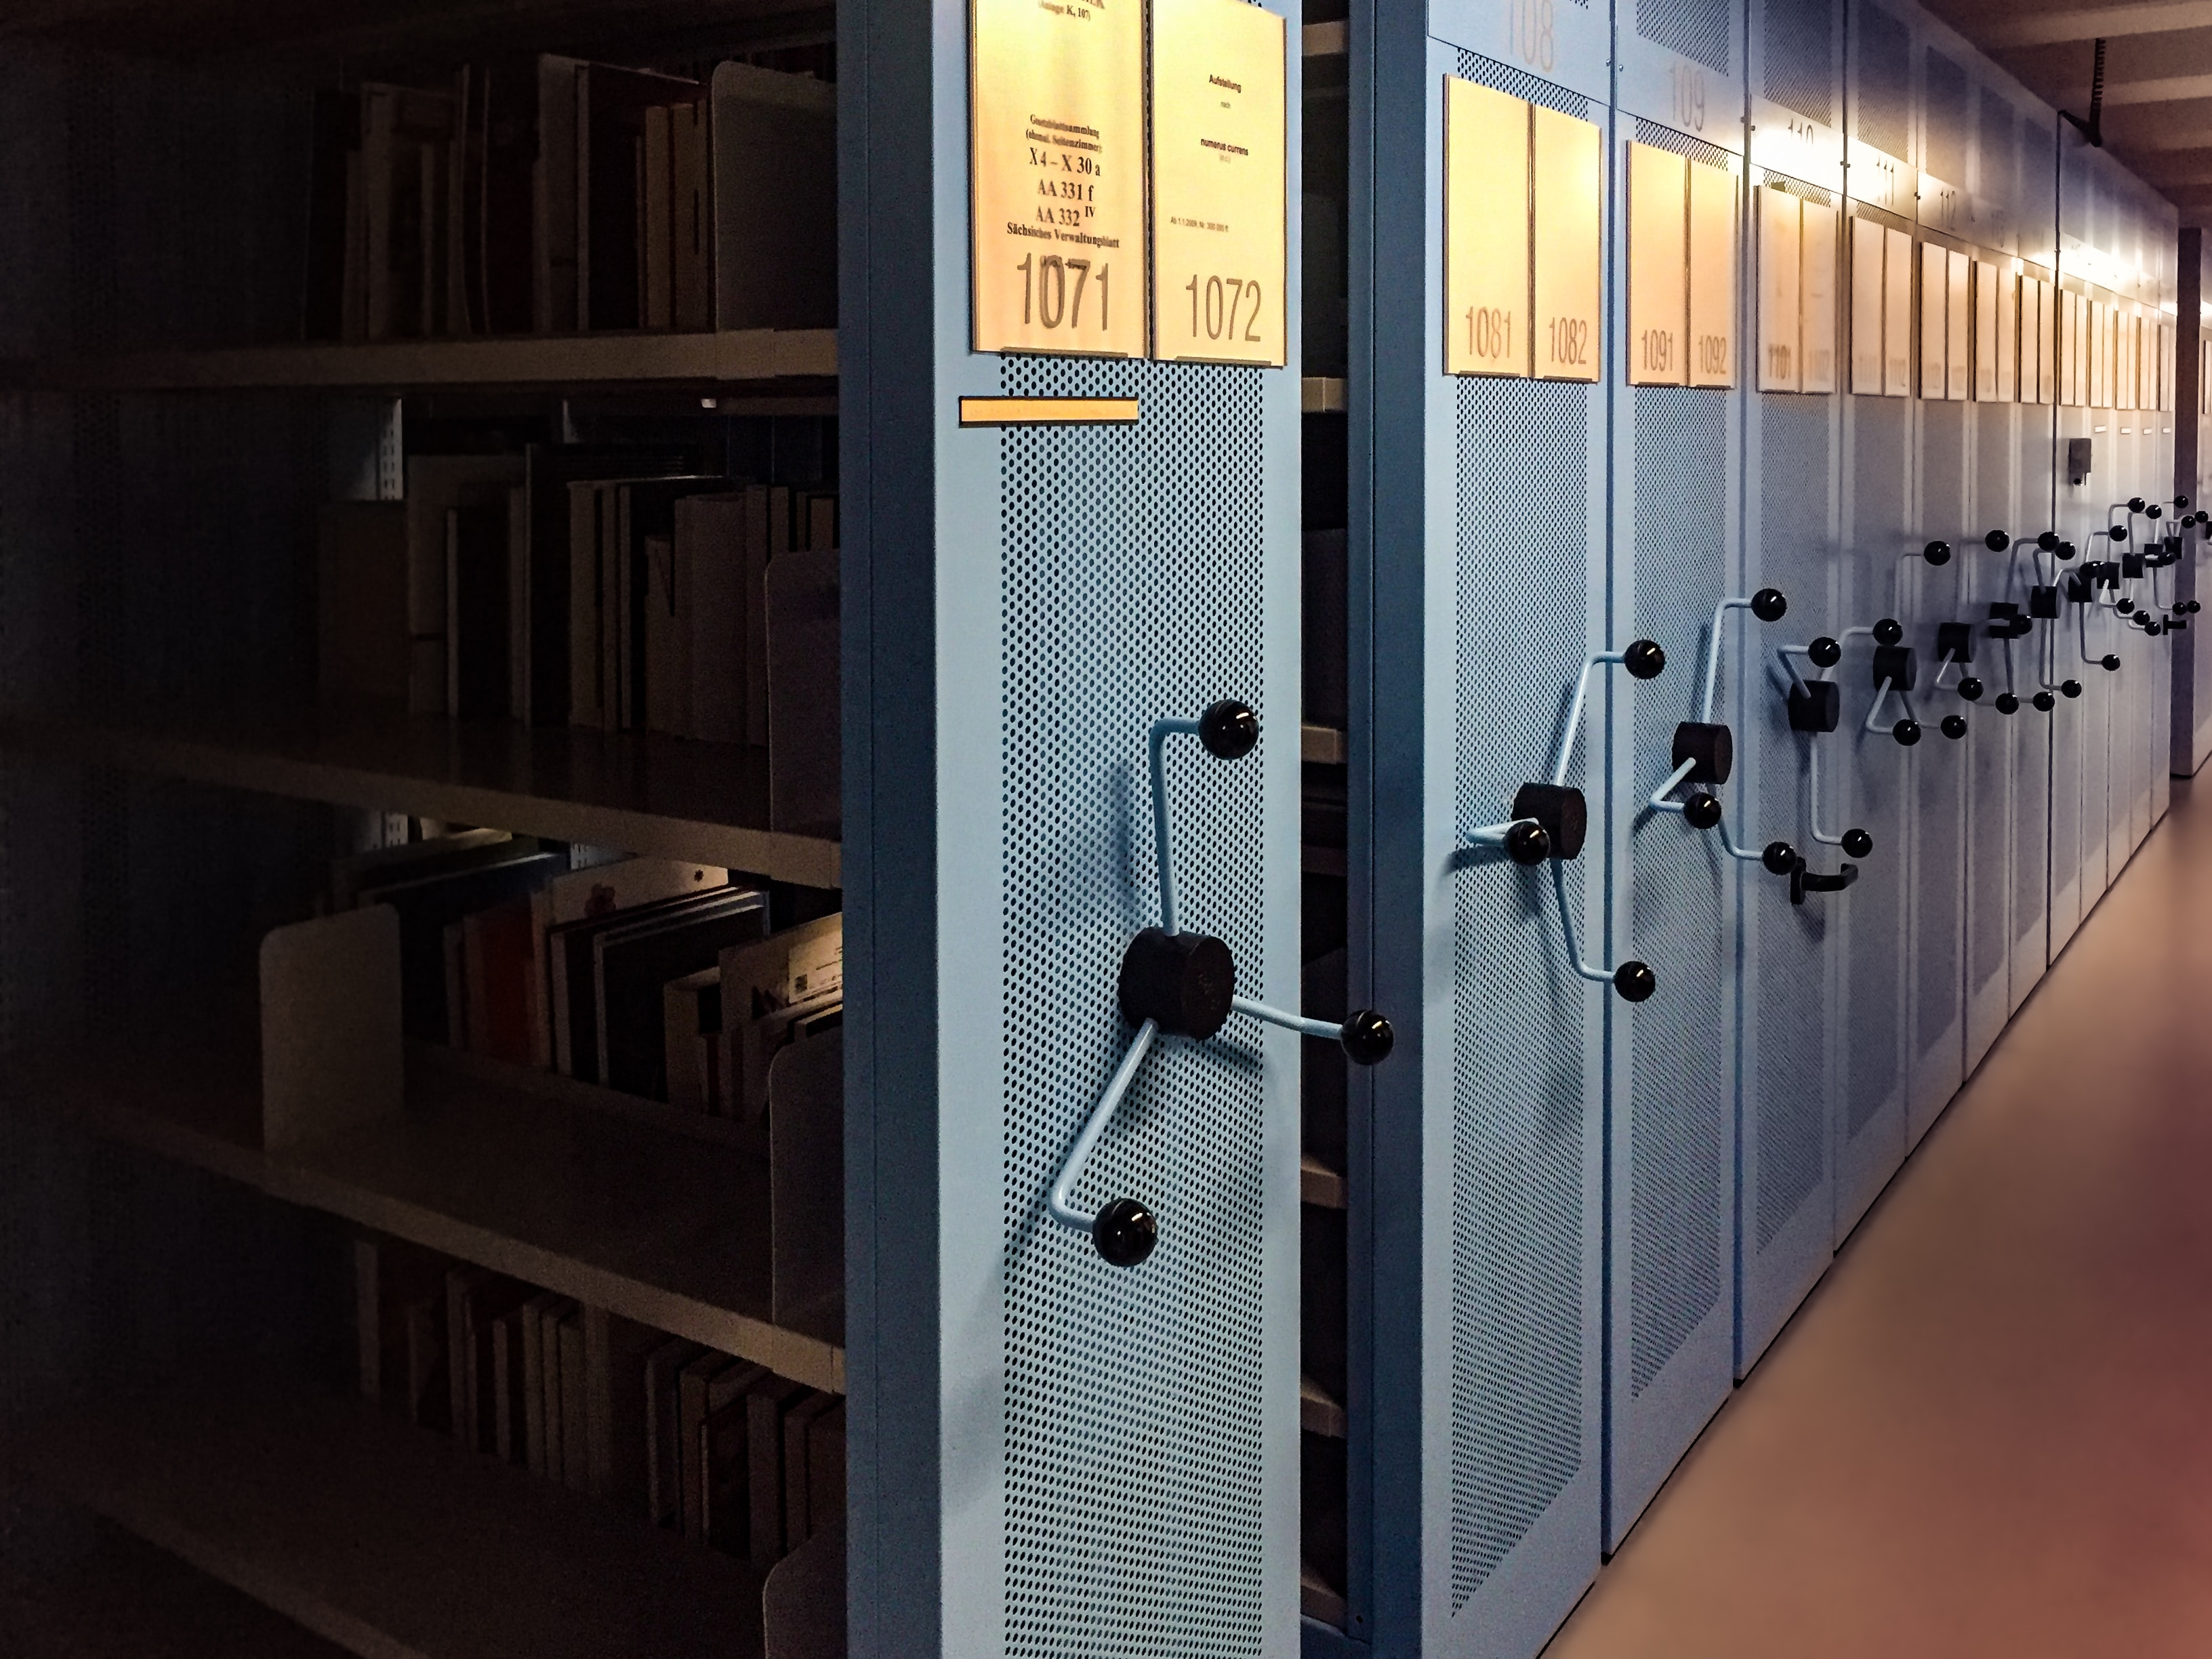
\includegraphics{archive-title-image}}
\advisor{Dr. Simon Kramer}
\coadvisor{Frank Helbling}
%\projectpartner{proj partner}
%\expert{Some expert}
\degreeprogram{Project 1}
\setupSignature{
	N. Dora={
\includegraphics[width=.5\linewidth]{./pictures/sig_Dora.png}},
	A. Vejseli={
\includegraphics[width=.5\linewidth]{./pictures/sig_Vejseli.png}},
	K. Wampfler={
\includegraphics[width=.5\linewidth]{./pictures/sig_Wampfler.png}}
}


%----------------  BFH tile page   -----------------------------------------
\maketitle
%------------ ABSTRACT        ----------------
\addchap{Abstract}
The URL-Archiver is a platform-independent Java application which specializes in extracting and archiving URLs from Unicode text or PDF files. It supports archiving on Archive Today and the Wayback Machine, with options to export archived URLs into CSV or the original Bibtex files. The application was developed with a focus on simplicity, modularity and self-explanatory code.

This report details the development process of the URL-Archiver, explaining the implementation strategies, SCRUM methodology and challenges overcome, and concludes with a outlook on potential future enhancements.

%------------ TABLEOFCONTENTS ----------------
\tableofcontents

%------------ List of Tables -------------
\listoftables

%------------ List of Figures ------------
\listoffigures

%------------ List of Listings -----------
\lstlistoflistings

%------------ START MAIN PART ------------
\mainmatter

\chapter{Introduction}
\section{Initial Situation}
The Internet is constantly evolving, which means that there is no guarantee that a website as it exists today will still exist in a few years' time, let alone contain the same information. While this might not be a concern that the average Internet user has to grapple with, it poses a challenge to the academic demographic, where it becomes crucial to reference sources and potentially integrate links to additional data. If links become inactive, verifying the sources becomes challenging, if not impracticable.

Archiving the existing status of a website is achievable, but it currently necessitates a manual and hence time-intensive operation, which not many people take the time to do. The objective of this project is to devise an automated solution to this predicament that is independent of platforms.

The stakeholders for this solution include:
\begin{itemize}
	\item Legal professionals and researchers who need to preserve web content as evidence or for case study references.
	\item Journalists and media agencies that require archiving web pages for future reporting or fact-checking.
	\item Librarians and archivists tasked with the digital preservation of online materials for historical records.
	\item Content creators and marketers who wish to maintain records of web content for portfolio or audit purposes.
	\item Educators and students who need to collect and cite online resources for academic projects and research.
	\item Organizations and businesses that need to archive their web presence for compliance and record-keeping.
\end{itemize}


\section{Poduct Goal}
The product goal is a platform independent Java application called ``URL-Archiver``.
The application must be Free/Libre and Open Source Software (FLOSS) licensed and fulfil the following functionalities:
\begin{enumerate}
    \item The software should be CLI\footnote{Command Line Interface}-based and offer a clear command line.
    \item The software should allow the user to input a path, which can be a folder or any Unicode text file.
    \item The software examines the contents of a file or folder to extract any web URLs using a standard regular expression or similar method.
    \item If desired, URLs can be automatically opened in a web browser.
    \item The extracted URLs are archived on archive.today and/or web.archive.org (known as The Wayback Machine) as per the user's preference.
    \item The software outputs the resulting archive URLs to the user.
    \item The software generates a CSV file containing the original URL and the archived Version of the URL.
    \item Optionally, the archived Versions are written back into the provided .bib file.
\end{enumerate}
The product goal is achieved if the software covers all the functionality listed above.
Furthermore, the code should be minimalistic, modular, and self-explaining.
In addition to the code, it is essential that the following documents are provided:
\begin{itemize}
    \item User manual
    \item Installation instructions (including installation script)
    \item Software documentation
\end{itemize}

\section{Priorities}
The following priorities are listed in order of importance:
\begin{enumerate}
    \item \textbf{Functionality}: The primary priority is the accurate extraction and archiving of URLs. The software should reliably identify URLs in varied file types and ensure their successful archiving on \href{https://archive.ph}{https://archive.ph} or \href{https://web.archive.org/save/}{Wayback Machine}.
    \item \textbf{Usability}: Given the diverse potential user base, the program should be platform-independent and possess a user-friendly interface. While the underlying mechanisms may be complex, the user experience should be seamless and intuitive.
    \item \textbf{Code Quality}: Emphasis should be placed on writing clean, minimal, and modular code. This not only aids in potential future enhancements but also in debugging and troubleshooting.
    \item \textbf{Documentation}: As with any software project, proper documentation is paramount. The project report should be concise, adhering to the principle of being ``maximally informative, minimally long,`` ensuring clarity of information without overwhelming the reader.
    \item \textbf{Integration with Existing File Types}: The ability to seamlessly insert archived URLs into .BIB files is a priority, given the potential academic applications of the software.
\end{enumerate}

\chapter{Specification}
\section{System Delimitation}

\subsection{System Environment (statics)}
\subsubsection{System Overview}
The primary purpose of the URL-Archiver is to extract URLs from Unicode text files and PDFs, and archive them on supported platforms: Archive.today and the Wayback Machine. The system provides the archived URL versions to the user via a CSV file. Additionally, when a .bib file is provided by the user, the original bib file is updated with a note field containing these archived URLs for each entry.

\subsubsection{Hardware Specifications}
The URL-Archiver does not impose any special hardware requirements. However, an internet connection is essential for the archiving process to function.

\subsubsection{Software Components}
The URL-Archiver is platform-independent, operating on major systems such as Windows (tested on Windows 10, version 22H2  and Windows 11, version 23H2), macOS (tested on macOS Sonoma), and Linux (tested on Ubuntu 20.04.3 LTS). The system has varying browser dependencies based on the operating system: Chrome is required for macOS, Edge for Windows, and Firefox for Ubuntu/Linux (Latest stable versions of the browsers are recommended). Users can change the default Browser in the configuration of the application. Other dependencies are installed with the URL-Archiver and do not require separate installation.

\subsubsection{System Architecture}
The URL-Archiver uses the Model-View-Controller (MVC) pattern, as illustrated in figure \ref{fig:mvc_highlevel}, to enable future enhancements, such as adding a GUI interface. The Factory pattern is applied where appropriate to simplify the extension of functionalities. For instance, adding extra archiving services can be easily accomplished by introducing a new archiving service, as shown in figure \ref{fig:factory_pattern_archiving_services}.

\begin{figure}
	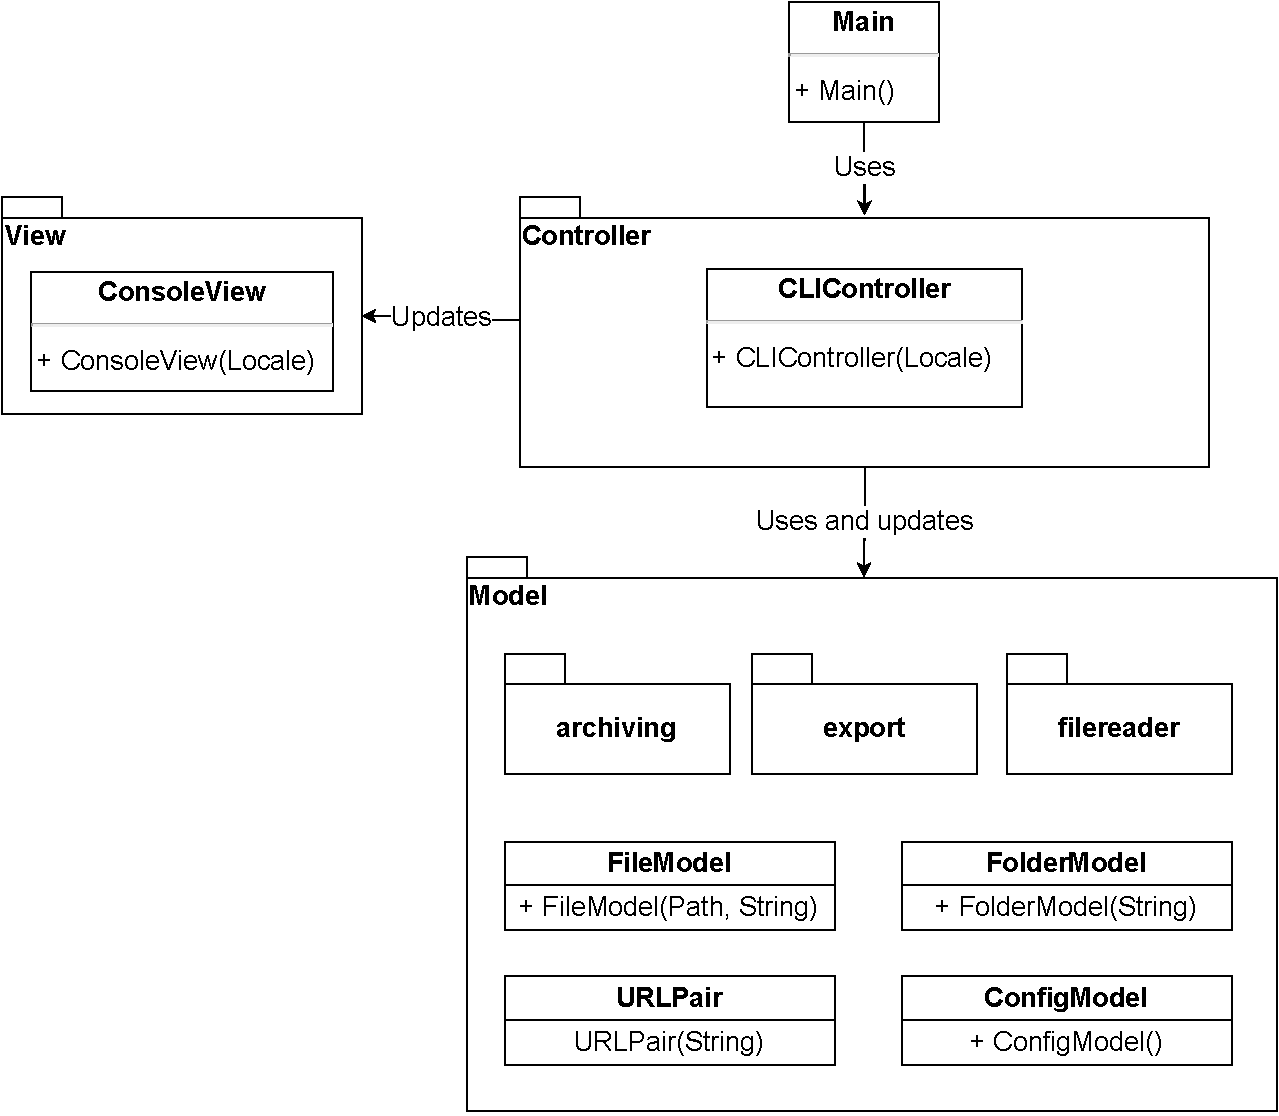
\includegraphics[width=0.5\textwidth]{./diagrams/mvc_diagram-Highlevel_MVC.pdf}
	\centering
	\caption{High-level MVC-Pattern from URL-Archiver}
	\label{fig:mvc_highlevel}
\end{figure}

\begin{figure}
	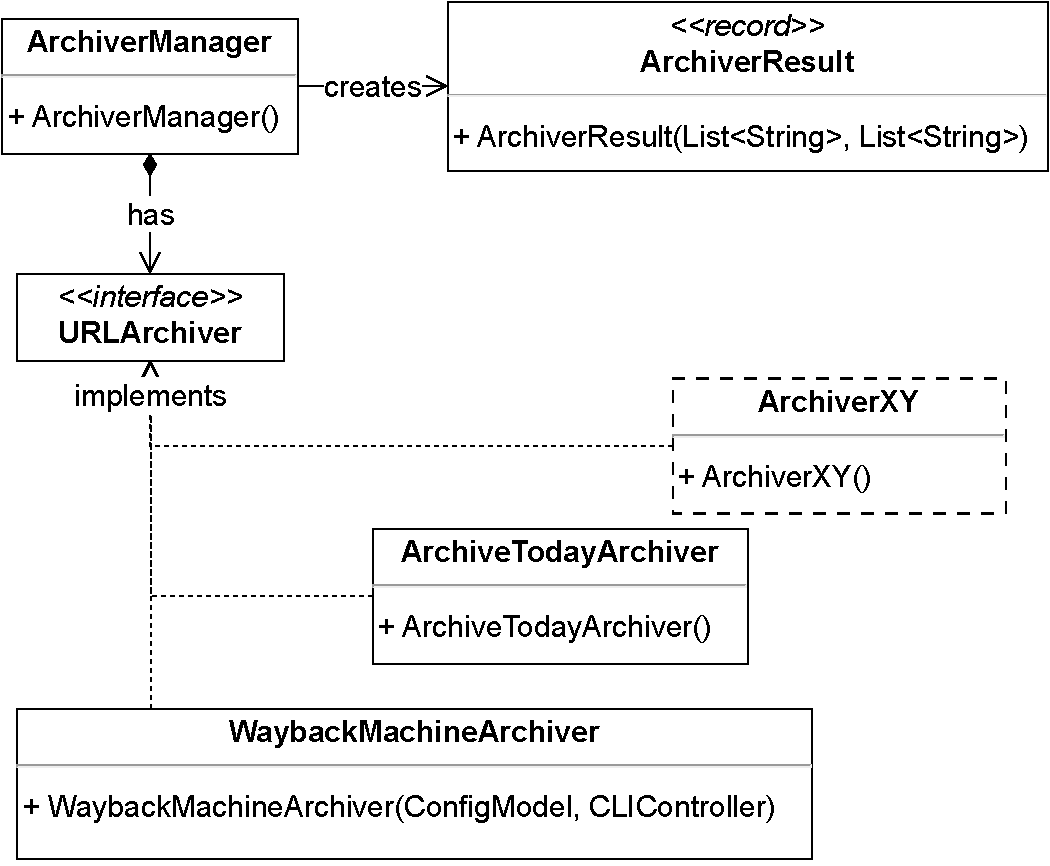
\includegraphics[width=0.5\textwidth]{./diagrams/URL_Archiver_Class_Diagram-ArchiverManager.pdf}
	\centering
	\caption{Extension with new archiving service XY (using the factory pattern)}
	\label{fig:factory_pattern_archiving_services}
\end{figure}

\subsubsection{Data Management}
Upon completion of its execution, the URL-Archiver generates a CSV file where each line contains an extracted URL and its archived versions, separated by semicolons. For example, a line like \texttt{https://xy.com;https://web.archive.org/xy;https://archive.ph/xy} shows the original URL and its archives. This simple format makes it easy to track and manage archived URLs. 

Optionally, if the user provided a \gls{BibTeX} file, URLs are integrated into the note field of each entry. If there's no existing note field, a new one is created with the format \texttt{note = {Archived Versions: \url{url1}, \url{url2}}}. If a note field already exists, the archived URLs are appended to it in the format \texttt{note = {<current note>, Archived Versions: \url{url1}, \url{url2}}}. This approach ensures that the archived URLs are neatly added to the BibTeX entries, maintaining the integrity of the original data.

\subsubsection{User Interface}
Currently, the system uses a command-line interface. The MVC pattern lays the groundwork for potential future implementation of a GUI interface.

\subsubsection{Integration with Other Systems}
The system integrates with the Wayback Machine via API, with certain limitations detailed in their API documentation\footnote{https://archive.org/details/spn-2-public-api-page-docs/mode/2up}. For archiving on Archive.today, which lacks an API, Selenium is used to automate the process as much as possible. However, users must manually complete captchas.

\subsubsection{Maintenance and Support}
Currently, there are no specified maintenance requirements or a support framework for the URL-Archiver.


\subsection{Process Environment (dynamics)}


\subsection{Operational Processes}
The URL-Archiver is initiated by the user, who provides a path to Unicode text or PDF files or a directory that contains such files. The application extracts URLs from these files and presents them sequentially to the user. The user then has options to open or archive that URL. He has also the following other options: 
\begin{itemize}
	\item \textbf{s}: Show a list of previously archived URLs.
	\item \textbf{u}: Update and view pending archive jobs.
	\item \textbf{n}: Navigate to the next URL.
	\item \textbf{q}: Quit the application.
	\item \textbf{c}: Change application settings.
	\item \textbf{h}: Access the Help Menu for assistance.
\end{itemize}

Upon completion, the user is prompted to save URL pairs to a CSV file and, if a Bibtex file is provided, to write the archived URLs back into it. 


\subsubsection{Event Handling}
In the URL Archiver, user actions are efficiently facilitated through the main menu. When archiving a URL, users can select either the Wayback Machine or Archive.today. In addition, the 'c' option in the menu allows users to configure settings, including setting up API keys for the Wayback Machine and selecting a default browser. The application cleverly handles unsupported input and incorrect paths by prompting the user for the correct information or action. This ensures smooth operation and user guidance throughout the process.

\subsubsection{Life Cycle}
The URL-Archiver’s life cycle begins with launch and path input, proceeding to URL extraction and user interactions via the menu options, and ends with prompts for data saving upon completion. See the high-level process in figure \ref{fig:hl_operational_process}.

\begin{figure}[b]
	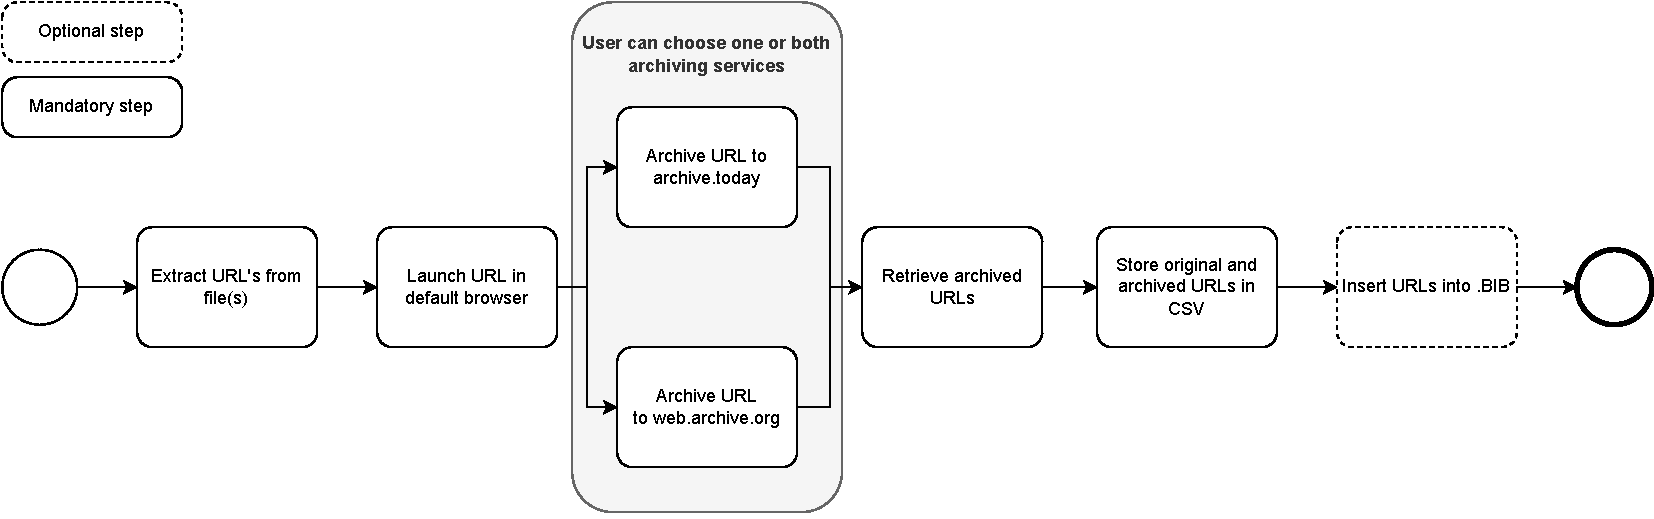
\includegraphics[width=1\textwidth]{./diagrams/process_model-simple-horizontal.pdf}
	\centering
	\caption{High-level operational process}
	\label{fig:hl_operational_process}
\end{figure}

\subsubsection{Error Management}
Errors within the URL-Archiver are caught and handled, typically prompting the user with a customized error message asking to retry the action. No system stack traces are shown to the user.

\subsubsection{Backup and Recovery}
Currently, there are no backup features; progress is not saved if the application ends unexpectedly, which is slated for future improvement.

\subsubsection{Update and Upgrade Policies}
Software updates require manual download and recompilation from the Git repository. The system does not provide automatic updates or an in-built feature for update checks.
\section{Requirements}

\subsection{Epics and User Stories}
In this section, we outline the main features (\glspl{Epic}) of the project and break them down into detailed user tasks (User Stories). This helps provide a clear understanding of the desired functions and behaviors of our software.
\subsubsection{Epic 1: File Input and Processing}
\textbf{Goal}: Allow the user to input various file types via the command line and prepare these files for further processing.
\begin{enumerate}
    \item \textbf{Prompt for File Path Input}
    \begin{itemize}
        \item \textbf{Description}: As a user, when I start the tool, I want to be prompted to input the path to my file, so the tool knows which file to process.
        \item \textbf{Acceptance Criteria}:
        \begin{itemize}
            \item Upon starting the tool, it prompts the user to enter a file path.
            \item On inputting an invalid path or if there are permissions issues, the tool provides a relevant error message.
        \end{itemize}
    \end{itemize}

    \item \textbf{Automatic File Type Detection}
    \begin{itemize}
        \item \textbf{Description}: As a user, I want the tool to automatically detect the file type (based on file extension) and treat it accordingly so that I don't need to specify the file type separately.
        \item \textbf{Acceptance Criteria}:
        \begin{itemize}
            \item The tool automatically identifies if the file is a .BIB, .TEX, .HTML, or .PDF.
            \item For unrecognized file types, the tool provides an appropriate error message.
        \end{itemize}
    \end{itemize}

    \item \textbf{Processing of Directories}
    \begin{itemize}
        \item \textbf{Description}: As a user, I want to input a whole directory, so the tool processes all supported files contained within.
        \item \textbf{Acceptance Criteria}:
        \begin{itemize}
            \item The tool can accept directory paths after the prompt.
            \item It processes all supported file types within the directory.
            \item The tool gives a message if files within the directory are skipped due to their type.
        \end{itemize}
    \end{itemize}

    \item \textbf{Processing Feedback}
    \begin{itemize}
        \item \textbf{Description}: As a user, I want to receive feedback when the tool starts processing the file and when it finishes, to know the status.
        \item \textbf{Acceptance Criteria}:
        \begin{itemize}
            \item A message is displayed when the processing of a file starts.
            \item Upon completion, a confirmation message is shown, which also includes any potential errors or warnings.
        \end{itemize}
    \end{itemize}
\end{enumerate}
\subsubsection{Epic 2: URL Detection and Extraction}
\textbf{Goal}: Accurately detect and extract URLs from input files for further processing.

\begin{enumerate}
    \item \textbf{Scan Files for URLs}
    \begin{itemize}
        \item \textbf{Description}: As a user, I want the system to scan my input files and identify any embedded URLs so that they can be extracted for archiving.
        \item \textbf{Acceptance Criteria}:
        \begin{itemize}
            \item System can detect URLs in a variety of file formats including .BIB, .TEX, .HTML, and .PDF.
            \item Detected URLs are listed without any duplication.
        \end{itemize}
    \end{itemize}

    \item \textbf{Use Regular Expressions for Extraction}
    \begin{itemize}
        \item \textbf{Description}: As a user, I want the system to use regular expressions or other reliable techniques to extract URLs so that all valid URLs are captured without error.
        \item \textbf{Acceptance Criteria}:
        \begin{itemize}
            \item System uses a robust regular expression pattern that matches most URL formats.
            \item Extracted URLs are validated to ensure they are in the correct format.
        \end{itemize}
    \end{itemize}

    \item \textbf{Store URL Line Number or Context}
    \begin{itemize}
        \item \textbf{Description}: As a user, when a URL is detected and extracted, I want the system to also store its line number or contextual information from the original file, enabling precise placement of its archived counterpart later on.
        \item \textbf{Acceptance Criteria}:
        \begin{itemize}
            \item Upon URL detection, the system captures and stores the line number or relevant context of the URL from the source file.
            \item This information is utilized later if archived URLs need to be placed back into the original files.
        \end{itemize}
    \end{itemize}


    \item \textbf{Compile a List of URLs}
    \begin{itemize}
        \item \textbf{Description}: After extraction, I want all URLs to be compiled into a single list, eliminating any duplicates, so that I have a clean list for archiving.
        \item \textbf{Acceptance Criteria}:
        \begin{itemize}
            \item The list contains all the unique URLs found in the input files.
            \item Invalid or broken URLs are flagged or removed from the list.
        \end{itemize}
    \end{itemize}
\end{enumerate}
\subsubsection{Epic 3: Web Browser Integration}
\textbf{Goal}: Seamlessly open detected URLs, one at a time, in a web browser for user verification, and immediately initiate the archiving process upon user decision.

\begin{enumerate}
    \item \textbf{Sequential URL Preview}
    \begin{itemize}
        \item \textbf{Description}: As a user, I want to preview each detected URL in my default browser sequentially to verify its content.
        \item \textbf{Acceptance Criteria}:
        \begin{itemize}
            \item System opens one URL at a time in the default browser.
            \item Immediately after the URL is displayed, the system presents the user with the option to archive.
        \end{itemize}
    \end{itemize}

    \item \textbf{Immediate Archiving Upon Decision}
    \begin{itemize}
        \item \textbf{Description}: After reviewing a URL in the browser, I want to decide if it should be archived. If I decide to archive, the system should immediately initiate the archiving process.
        \item \textbf{Acceptance Criteria}:
        \begin{itemize}
            \item System provides a prompt to accept or decline the archiving of the displayed URL.
            \item If the user chooses to archive, the system directly begins the archiving process, and the user may need to manually solve captchas.
        \end{itemize}
    \end{itemize}

    \item \textbf{Track Archiving Progress}
    \begin{itemize}
        \item \textbf{Description}: As a user, I want a clear indicator of how many URLs have been displayed, archived, and how many are left to process.
        \item \textbf{Acceptance Criteria}:
        \begin{itemize}
            \item The system displays a counter indicating the number of URLs already shown to the user.
            \item Another counter indicates how many URLs have been chosen for archiving.
            \item Yet another counter shows how many URLs remain to be processed/displayed.
        \end{itemize}
    \end{itemize}

    \item \textbf{Store User Decisions for Reporting}
    \begin{itemize}
        \item \textbf{Description}: As a user, after making a decision about archiving each URL, I want the system to store my choices so that they can be referred to or reported on later.
        \item \textbf{Acceptance Criteria}:
        \begin{itemize}
            \item The system maintains a record of each URL and the user's decision (archived or not archived).
            \item The stored decisions are available for any subsequent reporting needs.
        \end{itemize}
    \end{itemize}

\end{enumerate}
\subsubsection{Epic 4: Interaction with archive.ph}
\textbf{Goal}: Automate the process of archiving URLs via archive.ph while ensuring user interaction is seamless and all necessary data is captured for later use.

\begin{enumerate}
    \item \textbf{Automated URL Submission}
    \begin{itemize}
        \item \textbf{Description}: As a user, I want the system to automatically fill in the URL into the archive.ph input field and submit it for archiving.
        \item \textbf{Acceptance Criteria}:
        \begin{itemize}
            \item Upon initiation, system opens the archive.ph website in a browser.
            \item System auto-fills the given URL into the appropriate input field.
            \item System automatically triggers the submission process for archiving.
        \end{itemize}
    \end{itemize}

    \item \textbf{User Interaction for Captchas}
    \begin{itemize}
        \item \textbf{Description}: If required, I want to manually solve captchas to ensure the URL gets archived.
        \item \textbf{Acceptance Criteria}:
        \begin{itemize}
            \item If archive.ph presents a captcha, the system allows the user to solve it manually.
            \item The archiving process proceeds once the captcha is successfully solved.
        \end{itemize}
    \end{itemize}

    \item \textbf{Automatic Retrieval of Archived URL}
    \begin{itemize}
        \item \textbf{Description}: Once a URL is archived, I want the system to automatically retrieve and display the archived URL to me.
        \item \textbf{Acceptance Criteria}:
        \begin{itemize}
            \item System captures the new archived URL from archive.ph after the process completes.
            \item The archived URL is displayed to the user immediately.
            \item The archived URL is stored for later processing and reporting.
        \end{itemize}
    \end{itemize}
\end{enumerate}
\subsubsection{Epic 5: Output and Reporting}
\textbf{Goal}: Provide the user with an organized CSV file detailing URLs and their archived counterparts. Also, allow for integration of archived URLs back into supported input files.

\begin{enumerate}
    \item \textbf{Generate CSV File}
    \begin{itemize}
        \item \textbf{Description}: As a user, I want the system to produce a CSV file containing all original URLs and their corresponding archived URLs.
        \item \textbf{Acceptance Criteria}:
        \begin{itemize}
            \item A CSV file is generated upon completion of the archiving process.
            \item Each row in the CSV contains the original URL and its archived counterpart.
        \end{itemize}
    \end{itemize}

    \item \textbf{Integrate Archived URLs into Supported Files}
    \begin{itemize}
        \item \textbf{Description}: If desired, I want the system to insert the archived URL back into the original file, following its corresponding original URL.
        \item \textbf{Acceptance Criteria}:
        \begin{itemize}
            \item The system recognizes supported file types for this integration process.
            \item Upon user approval, the archived URL is inserted in the appropriate location (e.g., following its original URL) within the file.
        \end{itemize}
    \end{itemize}
\end{enumerate}
\clearpage
\subsection{Functional requirements}
The URL-Archiver project, as described in the original project description, which can be found in the Appendix (\ref{org_proj_desc}), is designed to be a platform-independent Java program that performs several key functions:

\begin{itemize}
    \item \textbf{Input Processing:} It accepts directories or files (including any Unicode-text- and PDF-Files) as input and scans them for URLs.
    \item \textbf{URL Extraction:} The program extracts all URLs using regular expressions.
    \item \textbf{Optional Browser Interaction:} It has an optional feature to open URLs in a web browser.
    \item \textbf{URL Archiving:} The program posts URLs to an archiving service (Archive Today \& The Wayback Machine) and retrieves the archived URLs.
    \item \textbf{Output Generation:} It outputs a CSV file containing the original and archived URL pairs.
    \item \textbf{Optional File Integration:} The program can optionally insert archived URLs into a .BIB file.
\end{itemize}

Additionally, the project emphasizes minimal, modular, and self-explanatory code. The report for the project is expected to be concise and include the original project description.

\subsection{Boundary}
The following limits apply:

\begin{itemize}
    \item \textbf{Input:} The application processes only Unicode-text-files (e.g.: .BIB, .TEX; .HTML; etc.) and PDF-files
    \item \textbf{Output:} The application exports the extracted and archived URLs in either CSV format or directly in a BIB file.
    \item \textbf{Archiving:} At present, the application should only support Archive Today and The Wayback Machine. Please refer to the documentation of the Wayback Machine\footnote{\href{https://archive.org/details/spn-2-public-api-page-docs/mode/2up}{API Documentation Wayback Machine}} or Archive Today\footnote{\href{https://archive.ph/faq}{FAQ of Archive Today}} for any restrictions on their APIs or services.
\end{itemize}
\clearpage
\subsection{Pre-conditions}
For the application to run smoothly, the following pre-conditions must be met:

\begin{itemize}
    \item \textbf{Java Environment:} The application necessitates the installation of Java Runtime Environment (JRE) version 21 on the system where it is intended to be executed.
    \item \textbf{File Formats:} The software is designed to operate with specific file formats, primarily Unicode text files and PDF files. It is necessary to provide these file types for successful operation.
    \item \textbf{Archiving Service Access:} The application requires internet connectivity and access to web archiving services, such as Archive Today, to enable its URL archiving functionality. \index{Archiving Services}
    \item \textbf{Login + S3 Credentials (Wayback Machine only):} To archive with the Wayback Machine, a login and S3 credentials are required.
\end{itemize}
\clearpage
\section{Usability}

\subsection{Personas}
This section introduces personas for the URL-Archiver, detailing diverse user profiles and their interactions with the application, to provide a understanding of its usability and functionality.

\subsection{Persona 1 - Alex Frei (Investigative Journalist)}

\subsubsection{Persona Overview}

\textbf{Name:} Alex Frei \\
\textbf{Age:} 32 \\
\textbf{Occupation:} Investigative Journalist \\
\textbf{Industry:} Media and News Reporting

\subsubsection{Background}
Alex is an experienced journalist specializing in political reporting.
Known for in-depth investigative pieces, Alex often covers high-stakes political events, requiring rapid access to historical web data for fact-checking.

\subsubsection{Goals}
\begin{itemize}
    \item Quickly archive web pages for timely reporting on political events.
    \item Maintain an archive of web pages for in-depth analysis and future reference.
    \item Retrieve archived URLs efficiently for referencing in articles and reports.
\end{itemize}

\subsubsection{Challenges}
\begin{itemize}
    \item Finding a tool that archives web pages instantly and reliably.
    \item Ensuring easy access and shareability of archived content.
    \item Managing a collection of archived URLs efficiently and effectively.
\end{itemize}

\subsubsection{Interactions with URL-Archiver}
\begin{itemize}
    \item Utilizes URL-Archiver's CLI for quick and efficient archiving.
    \item Values the open-source nature for trustworthiness in journalistic integrity.
    \item Relies on CSV output for organized referencing of archived content.
\end{itemize}

\subsection{Persona 2 - Dr. Emma Katrin Winter (Academic Researcher)}

\subsubsection{Persona Overview}

\textbf{Name:} Dr. Emma Katrin Winter \\
\textbf{Age:} 40 \\
\textbf{Occupation:} Academic Researcher \\
\textbf{Industry:} Higher Education

\subsubsection{Background}
Dr. Winter is a tenured professor focused on social sciences, often citing digital journals and data repositories.
She requires reliable digital archiving for scholarly citations and utilizes BibTeX files for managing bibliographic data.

\subsubsection{Goals}
\begin{itemize}
    \item Ensure accurate citation of web content in academic papers.
    \item Maintain and manage a digital archive of resources for teaching and research.
    \item Share archived content with academic peers for collaboration.
    \item Integrate archived URLs into BibTeX files for streamlined academic referencing.
\end{itemize}

\subsubsection{Challenges}
\begin{itemize}
    \item Needs a reliable method for archiving web pages.
    \item Seeks efficient integration of archived URLs into BibTeX files.
    \item Manages extensive digital archives for large-scale research projects.
\end{itemize}

\subsubsection{Interactions with URL-Archiver}
\begin{itemize}
    \item Uses URL-Archiver for capturing and archiving academic papers.
    \item Values the integration of archived URLs into BibTeX files for academic referencing.
    \item Relies on CSV file generation for organizing digital resources.
\end{itemize}

\subsection{Persona 3 - Michael Schwarz (Content Marketing Specialist)}

\subsubsection{Persona Overview}

\textbf{Name:} Michael Schwarz \\
\textbf{Age:} 35 \\
\textbf{Occupation:} Content Marketing Specialist \\
\textbf{Industry:} Digital Marketing

\subsubsection{Background}
Michael is a skilled content marketer, responsible for digital campaigns and web presence analytics in a dynamic marketing agency.
His role involves archiving web content for brand reputation management and competitive analysis.

\subsubsection{Goals}
\begin{itemize}
    \item Regularly archive web content for marketing audits and compliance.
    \item Manage a digital archive for campaign retrospectives.
    \item Ensure easy access to archived content for reviews and strategic planning.
\end{itemize}

\subsubsection{Challenges}
\begin{itemize}
    \item Needs a tool capable of archiving web content efficiently.
    \item Requires a streamlined process for accessing archived material.
    \item Seeks an archive system that is user-friendly and reliable.
\end{itemize}

\subsubsection{Interactions with URL-Archiver}
\begin{itemize}
    \item Regularly uses URL-Archiver for archiving online marketing content.
    \item Appreciates the CLI interface for ease and speed of use.
    \item Relies on the tool's capability to create organized audit trails.
\end{itemize}
\clearpage

\subsection{Storyboard}
In this section, we present the storyboard for the URL-Archiver, illustrating the user's interaction with the application.
Through the sketches~\ref{fig:StoryBoard_1} to~\ref{fig:StoryBoard_8}, we show the user's journey from the initial greeting in the console to the final archiving of URLs.
This story concentrate on the user's experience, the steps they take, and the decisions they make, rather than the precise UI design details.

\begin{figure}[h!]
    \centering
    
\includegraphics[width=1\textwidth]{pictures/Story Board/StoryBoard_1}
    \caption{The console greets Bob with a straightforward interface, presenting the archiving options. Bob opts to begin the archiving process.}
    \label{fig:StoryBoard_1}
\end{figure}
\begin{figure}[h!]
    \centering
    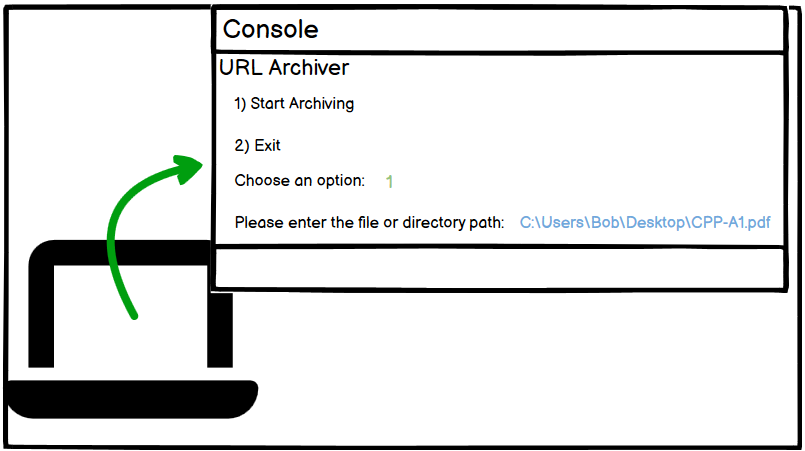
\includegraphics[width=1\textwidth]{pictures/Story Board/StoryBoard_2}
    \caption{Bob is prompted to enter the file or directory path. He types in the path to the PDF document that contains the URLs he wishes to archive.}
    \label{fig:StoryBoard_2}
\end{figure}
\begin{figure}[h!]
    \centering
    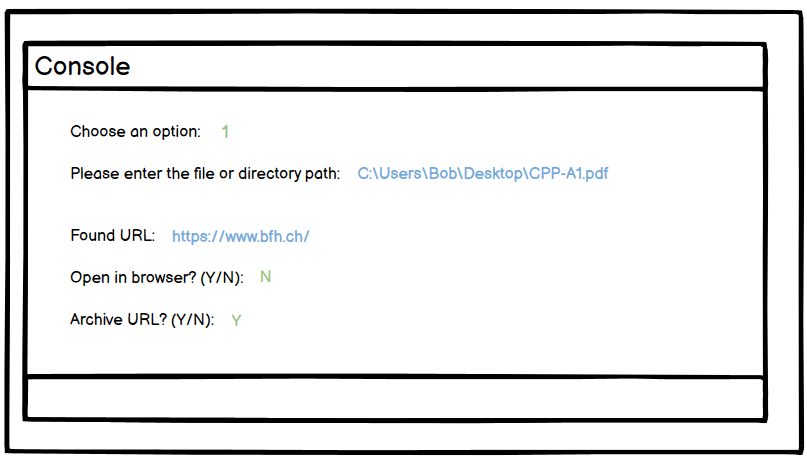
\includegraphics[width=1\textwidth]{pictures/Story Board/StoryBoard_3}
    \caption{Upon processing the input, the URL-Archiver quickly finds the first URL within the document. The console inquires if Alex wants to open it in a web browser or proceed with archiving. Alex decides not to open the URL in the browser and instead chooses to archive it directly.}
    \label{fig:StoryBoard_3}
\end{figure}
\clearpage

\begin{figure}[h!]
    \centering
    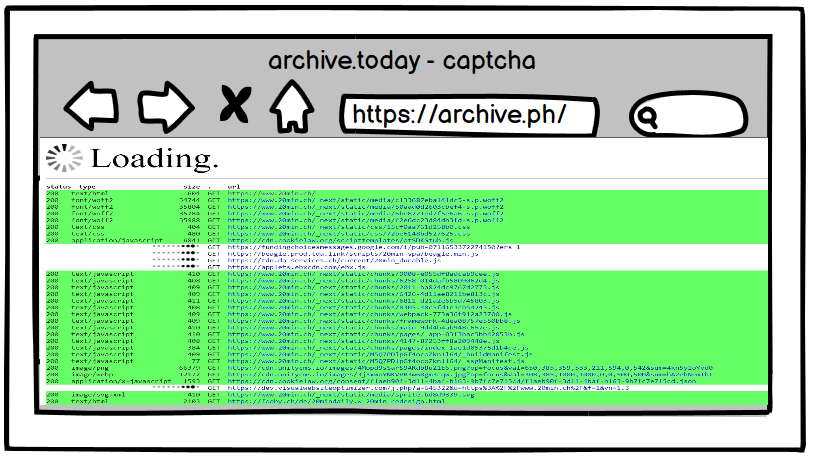
\includegraphics[width=1\textwidth]{pictures/Story Board/StoryBoard_4}
    \caption{The Archiver initiates the archiving process. A loading screen appears, indicating that the Archive Today platform is working on capturing the webpage.}
    \label{fig:StoryBoard_4}
\end{figure}
\begin{figure}[h!]
    \centering
    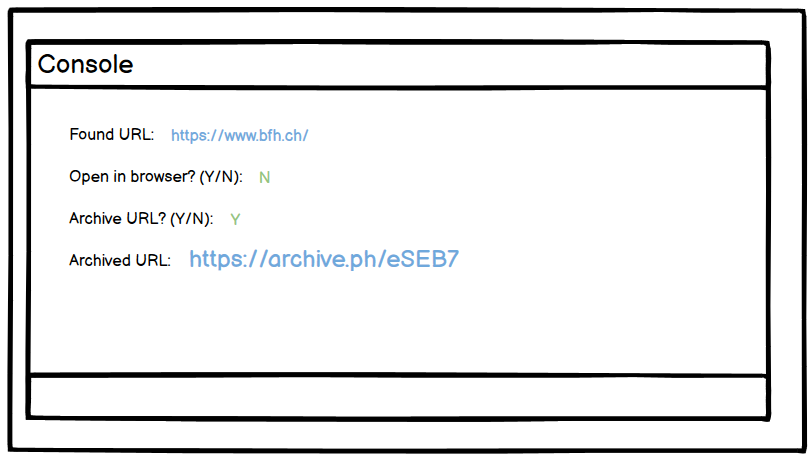
\includegraphics[width=1\textwidth]{pictures/Story Board/StoryBoard_5}
    \caption{The first URL is archived, and the Archiver outputs the archived link.}
    \label{fig:StoryBoard_5}
\end{figure}
\begin{figure}[h!]
    \centering
    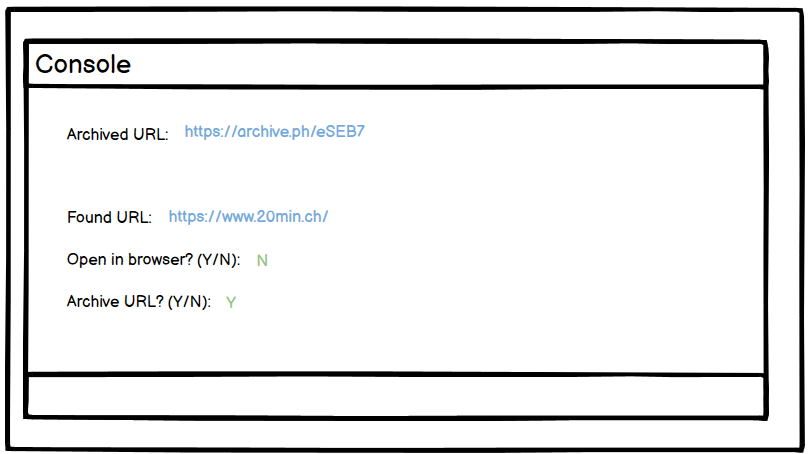
\includegraphics[width=1\textwidth]{pictures/Story Board/StoryBoard_6}
    \caption{The application moves to the next URL. Without hesitation, Bob decides to archive this one as well.}
    \label{fig:StoryBoard_6}
\end{figure}

\begin{figure}[h!]
    \centering
    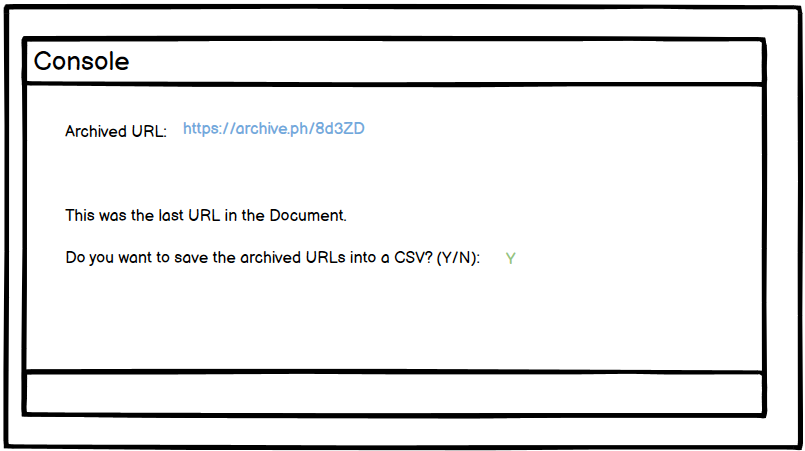
\includegraphics[width=1\textwidth]{pictures/Story Board/StoryBoard_7}
    \caption{The last URL is processed, and the Archiver asks Bob if he wants to save the list of archived URLs as a CSV file. Bob types "Y" to confirm.}
    \label{fig:StoryBoard_7}
\end{figure}
\begin{figure}[h!]
    \centering
    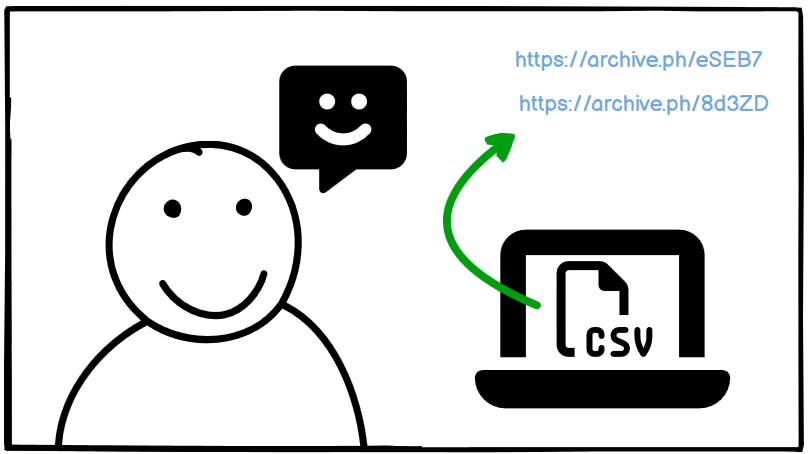
\includegraphics[width=1\textwidth]{pictures/Story Board/StoryBoard_8}
    \caption{Bob feels accomplished. The Archiver saved time, and the important URLs are now securely archived.}
    \label{fig:StoryBoard_8}
\end{figure}
\clearpage

\subsection{UX-Prototyping}
This section presents the initial version of our UX prototype for the URL-Archiver, created using Balsamiq\footnote{\href{https://balsamiq.com/}{Balsamiq} is a rapid wireframing tool that helps you work faster and smarter. It reproduces the experience of sketching on a whiteboard, but using a computer.}.
The series of UI sketches, from Figure~\ref{fig:Initial_Interface} through Figure~\ref{fig:Process_Continuation}, represent an early conceptualization of the application's user experience.
This prototype does not reflect the current state of the application, but serves as an important step in our design process.
Each figure illustrates the key stages of user interaction, from starting the application to completing the archiving process.

\begin{figure}[h!]
    \centering
    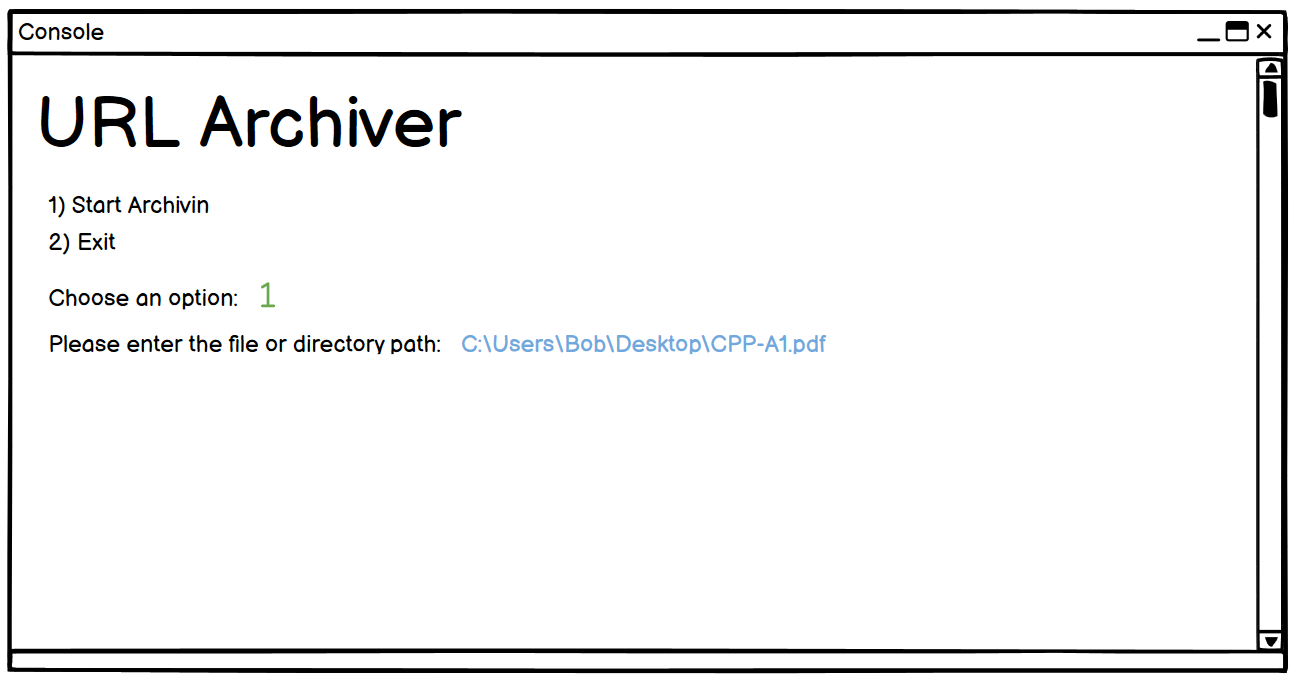
\includegraphics[width=1\textwidth]{pictures/UX-Prototype/Prototype_1}
    \caption{Starting point of the URL-Archiver where the user is prompted to begin archiving or exit the application.}
    \label{fig:Initial_Interface}
\end{figure}
\begin{figure}[h!]
    \centering
    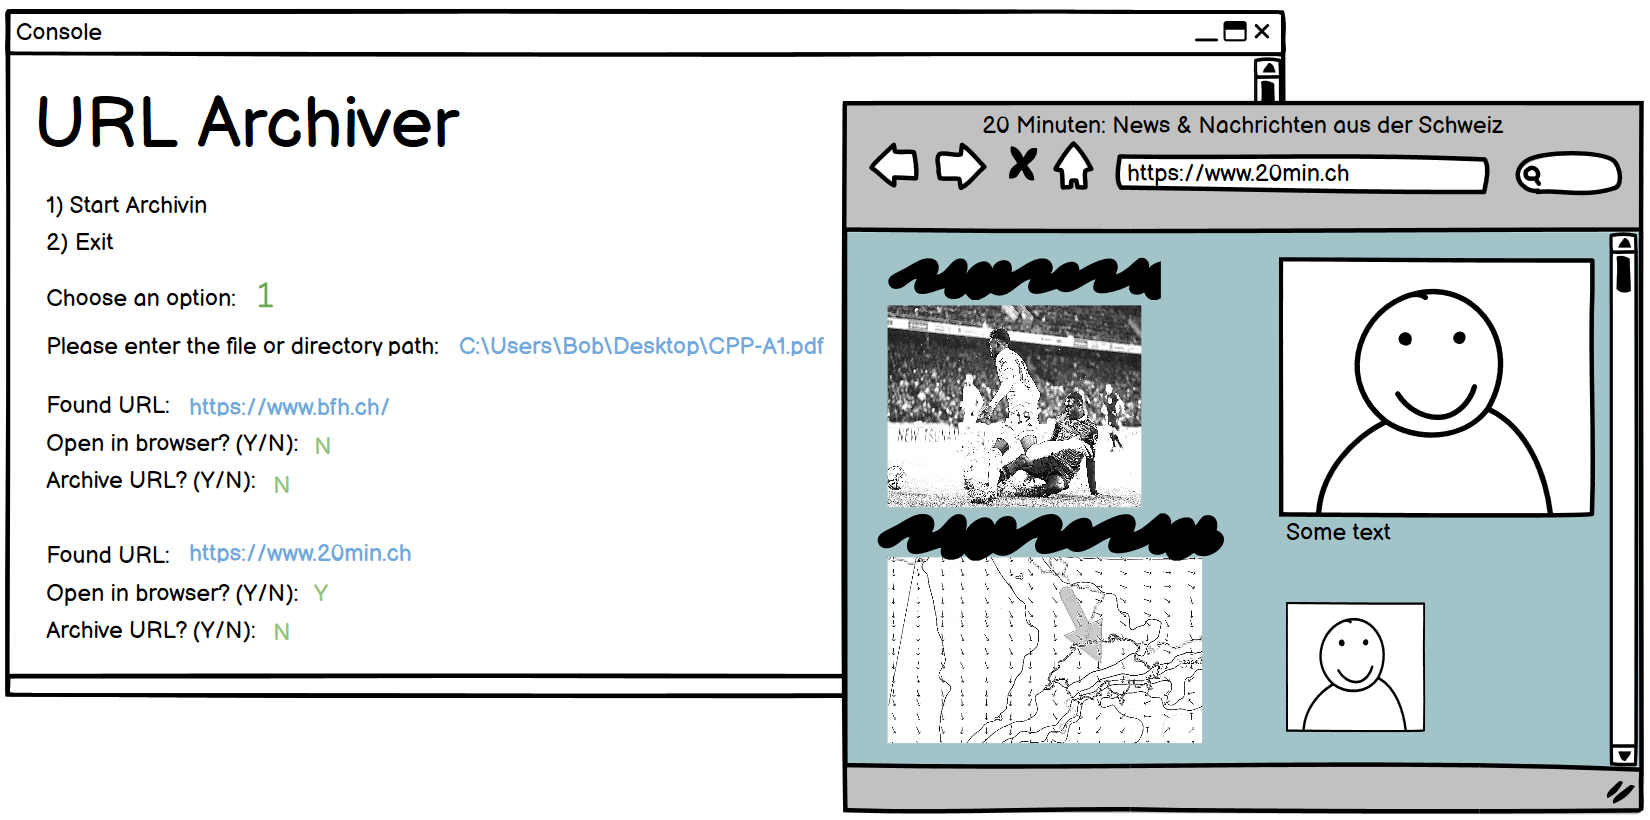
\includegraphics[width=1\textwidth]{pictures/UX-Prototype/Prototype_2}
    \caption{Upon choosing to open a URL in the browser, the user is presented with the live web page.}
    \label{fig:URL_Discovery}
\end{figure}
\begin{figure}[h!]
    \centering
    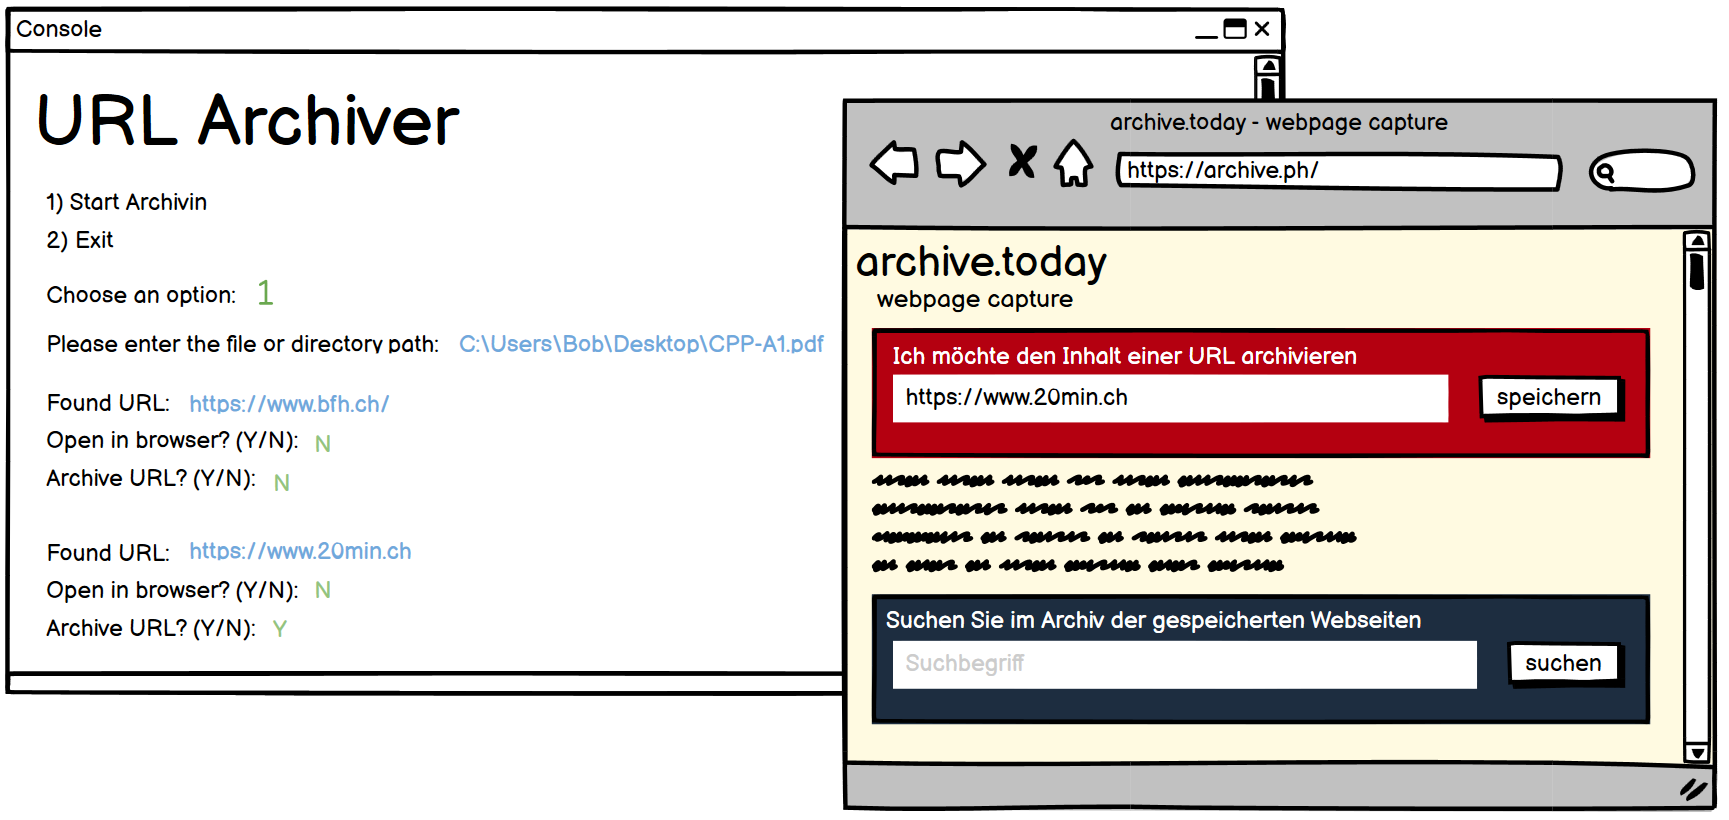
\includegraphics[width=1\textwidth]{pictures/UX-Prototype/Prototype_3}
    \caption{The user opts to archive the second URL, initiating the archiving process through the interface.}
    \label{fig:Browser_Interaction}
\end{figure}
\clearpage

\begin{figure}[h!]
    \centering
    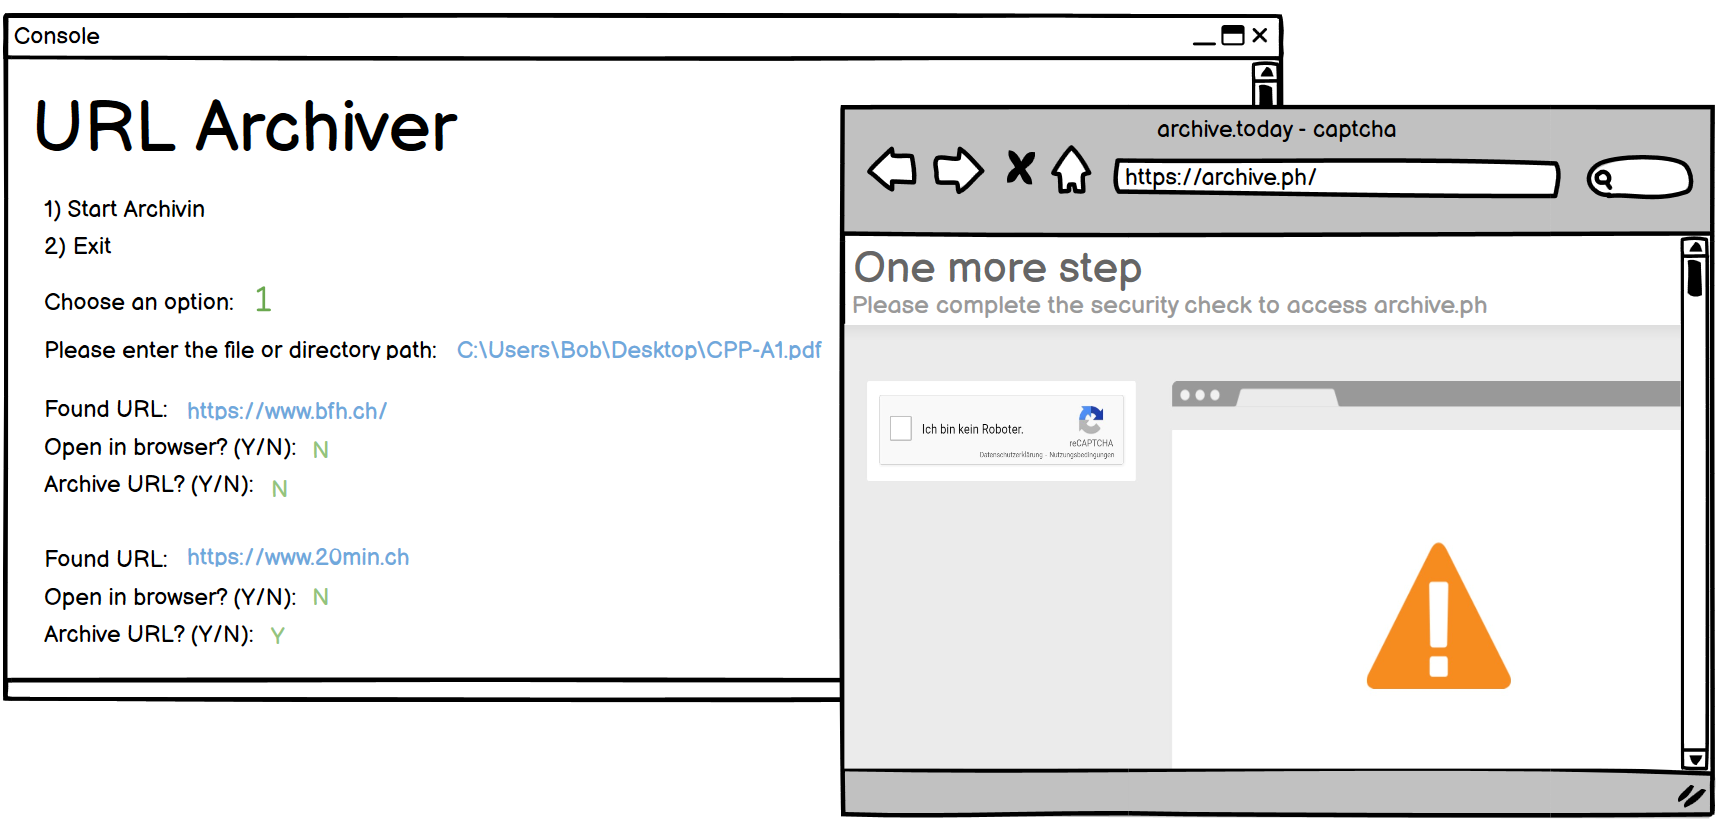
\includegraphics[width=1\textwidth]{pictures/UX-Prototype/Prototype_4}
    \caption{A security step requiring captcha verification to proceed with the archiving process.}
    \label{fig:Archiving_Decision}
\end{figure}
\begin{figure}[h!]
    \centering
    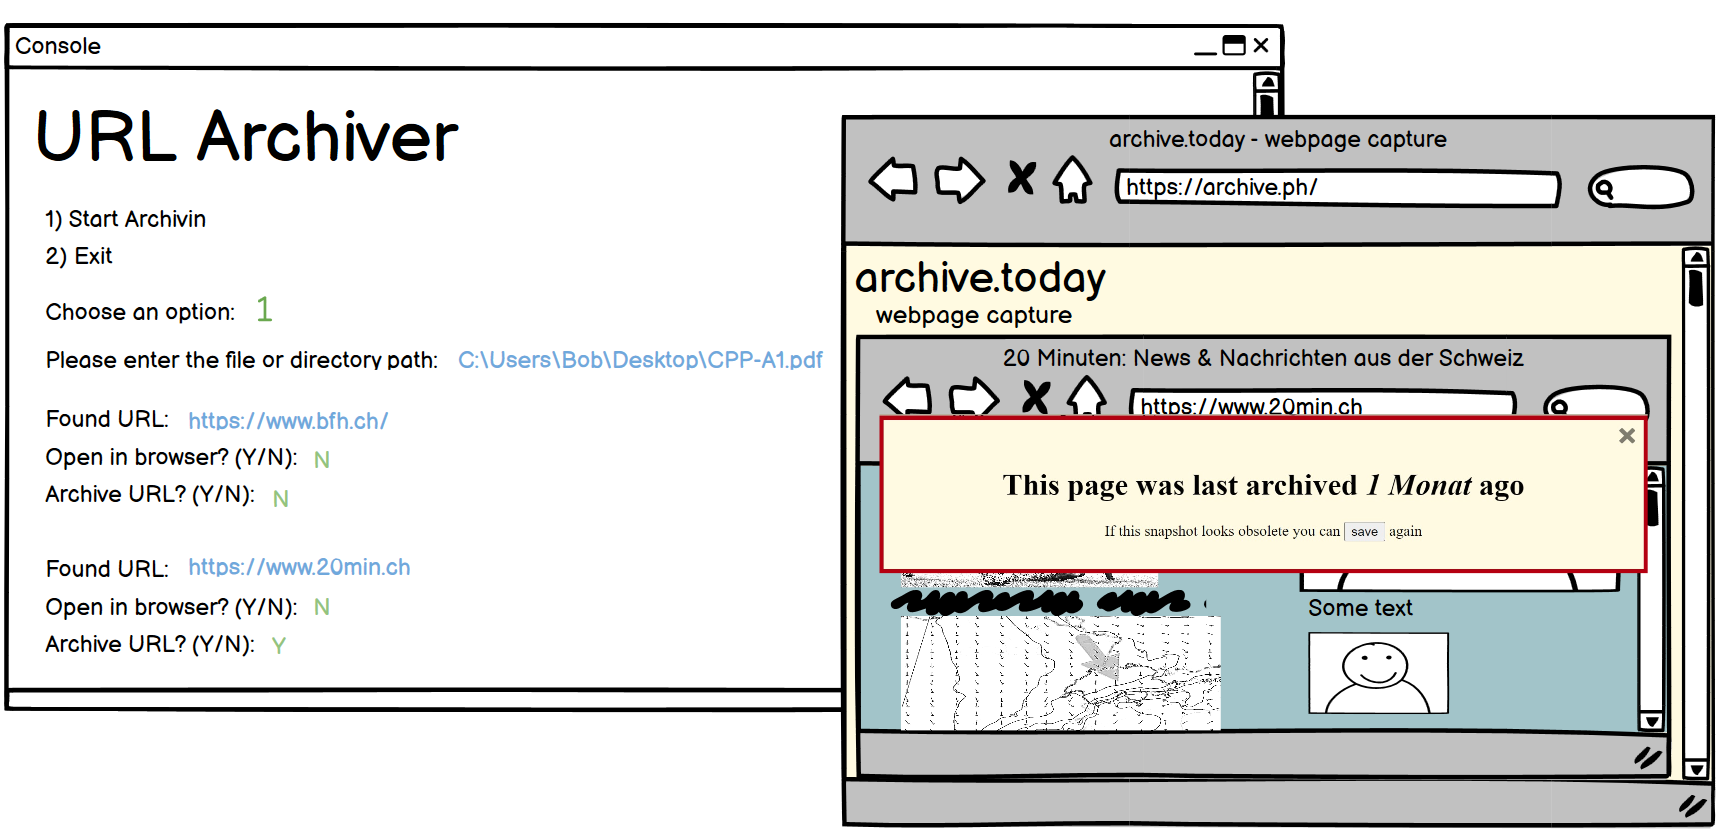
\includegraphics[width=1\textwidth]{pictures/UX-Prototype/Prototype_5}
    \caption{Archive Today informs that the website has been archived before. The application proceeds to re-archive the site.}
    \label{fig:Captcha_Verification}
\end{figure}
\begin{figure}[h!]
    \centering
    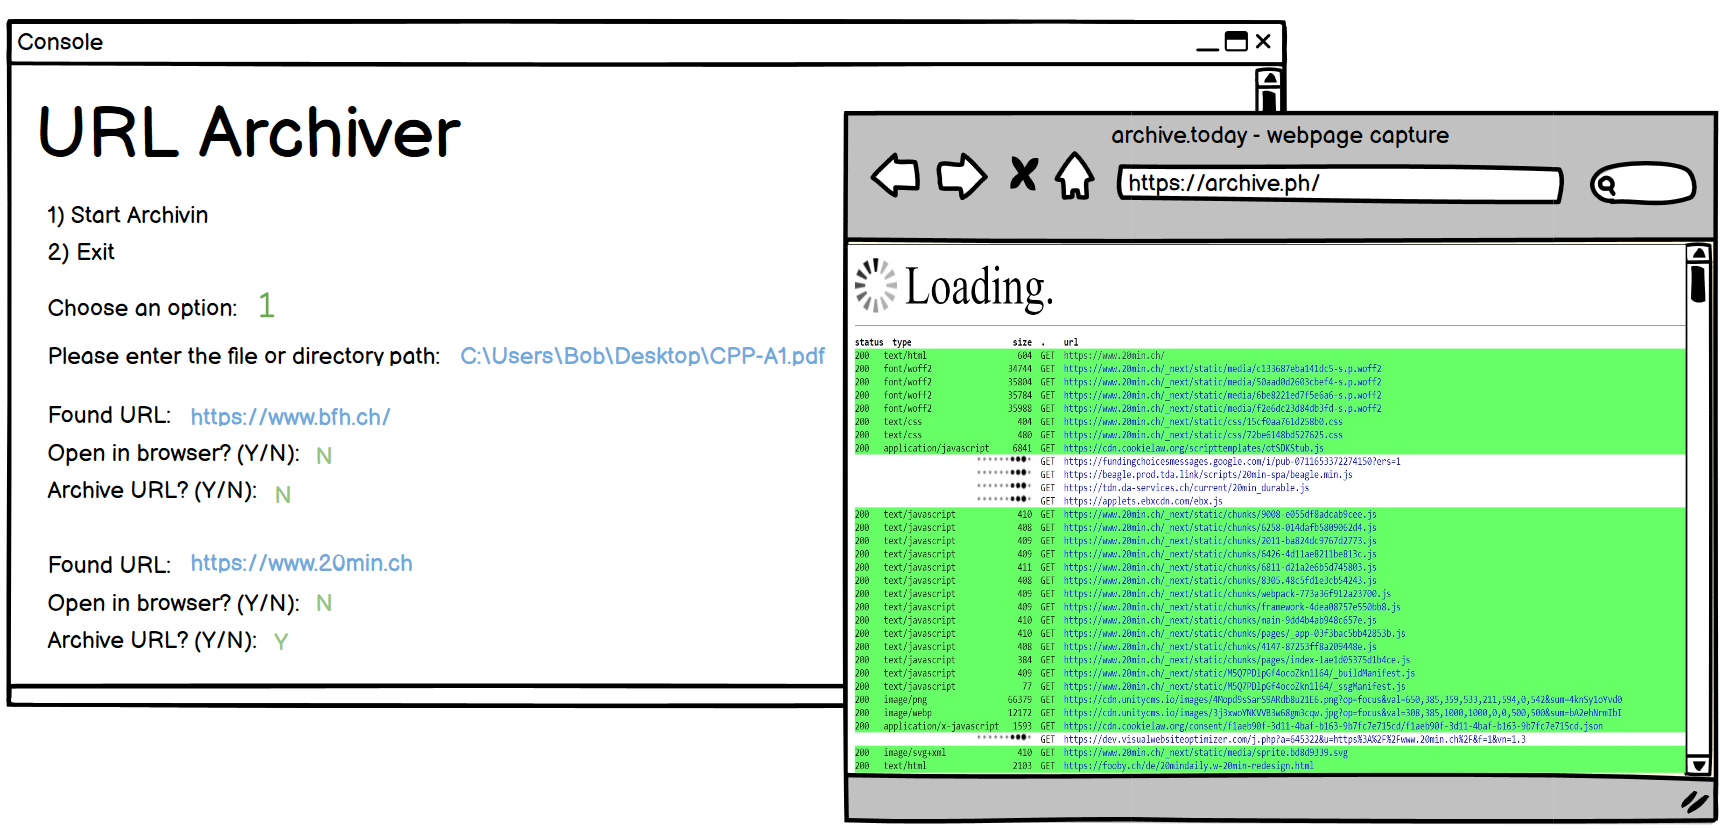
\includegraphics[width=1\textwidth]{pictures/UX-Prototype/Prototype_6}
    \caption{The archiving process is actively underway on the Archive Today platform.}
    \label{fig:Archiving_Confirmation}
\end{figure}
\begin{figure}[h!]
    \centering
    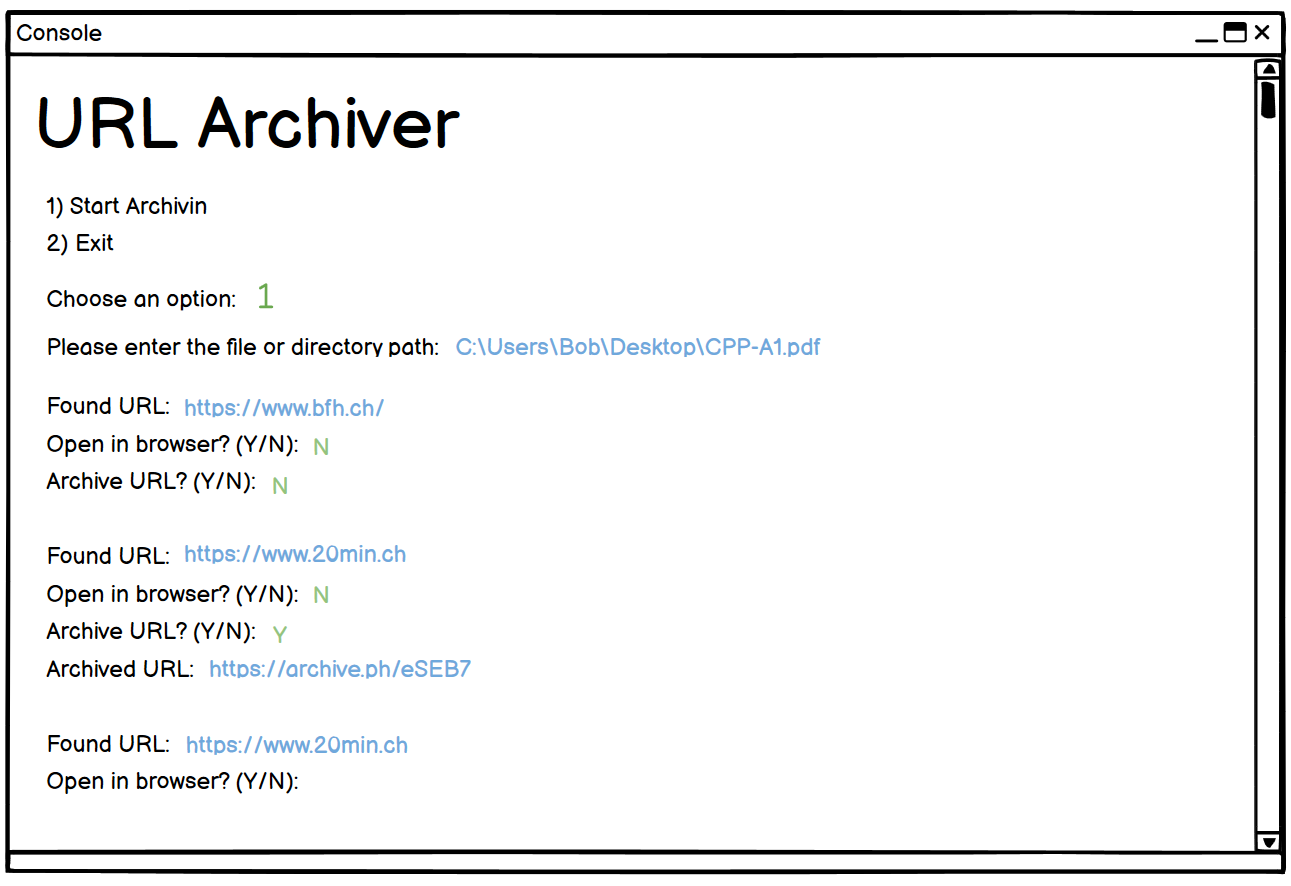
\includegraphics[width=1\textwidth]{pictures/UX-Prototype/Prototype_7}
    \caption{After successful archiving, the system provides the user with a confirmation message and the archived URL.}
    \label{fig:Process_Continuation}
\end{figure}
\clearpage


\chapter{Implementation}
\section{Architecture}
This chapter describes the architecture of the URL-Archiver. 

\subsection{Frontend}
The frontend architecture of the URL-Archiver is centered on a console-based interface, as evidenced by the \texttt{ConsoleView} and \texttt{CLIController} classes featured in Figure \ref{fig:MVC_Highlevel}.

The \texttt{ConsoleView} class is essential for presenting information and managing user input in a console setting. It is specifically designed to display data and messages clearly and in a user-friendly way. In parallel, the \texttt{CLIController}, a key component of the Controller segment in the MVC (Model-View-Controller) framework, serves as an intermediary between the \texttt{ConsoleView} and the application’s backend. This class efficiently processes user inputs from the \texttt{ConsoleView}, liaises with the model to retrieve or alter data, and then updates the console interface with these changes. This architecture is crafted to enable streamlined and effective user interactions within a command-line environment. The Figure \ref{fig:Screenshot_ConsoleView} illustrates the welcome message that the URL archiver displays to users. 
\vskip 0.5cm
\begin{figure}[h!]
    \center
    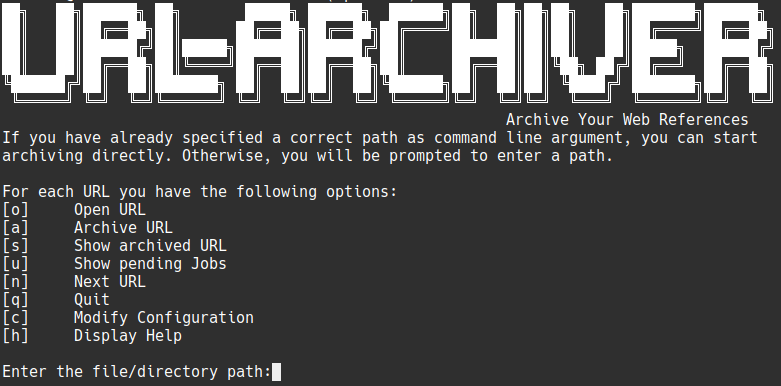
\includegraphics[width=1\textwidth]{pictures/final_presentation/command_line_application.jpg}
    \caption{Screenshot of the Console View}
    \label{fig:Screenshot_ConsoleView}
\end{figure}



\clearpage

\subsection{Backend}

\subsubsection{Software Architectural Design}
The URL-Archiver is developed following the principles of the MVC (Model-View-Controller) software architectural pattern. The MVC framework, as detailed in Figure \ref{fig:MVC_Highlevel}, is a structured approach to building user interfaces in software applications. It organizes an application into three interrelated components:

\begin{itemize}
	\item \textbf{Model:} This layer embodies the URL-Archiver's data structures, business logic, and operational rules. Components such as \texttt{FileModel}, \texttt{FolderModel}, \texttt{URLPair}, and \texttt{ConfigModel}, as shown in Figure \ref{fig:MVC_Highlevel}, represent the model.
	\item \textbf{View:} Tasked with rendering data from the model to the user and forwarding user commands to the controller. The \texttt{ConsoleView} in Figure \ref{fig:MVC_Highlevel} serves as a demonstration of this component.
	\item \textbf{Controller:} It is responsible for handling user inputs, engaging with the model to process data, and selecting the appropriate view for presentation. The \texttt{CLIController}, depicted in Figure \ref{fig:MVC_Highlevel}, is indicative of this segment.
\end{itemize}

This modular structure allows for an efficient separation of code, which aids in easier maintenance and streamlined development. The \texttt{Main} class operates as the launching point for the URL-Archiver, effectively coordinating the MVC pattern. Interaction between the Controller and the Model results in updates to the Model, with the View being refreshed in tandem to maintain a clear demarcation of responsibilities.

\begin{figure}[h!]
    \center
    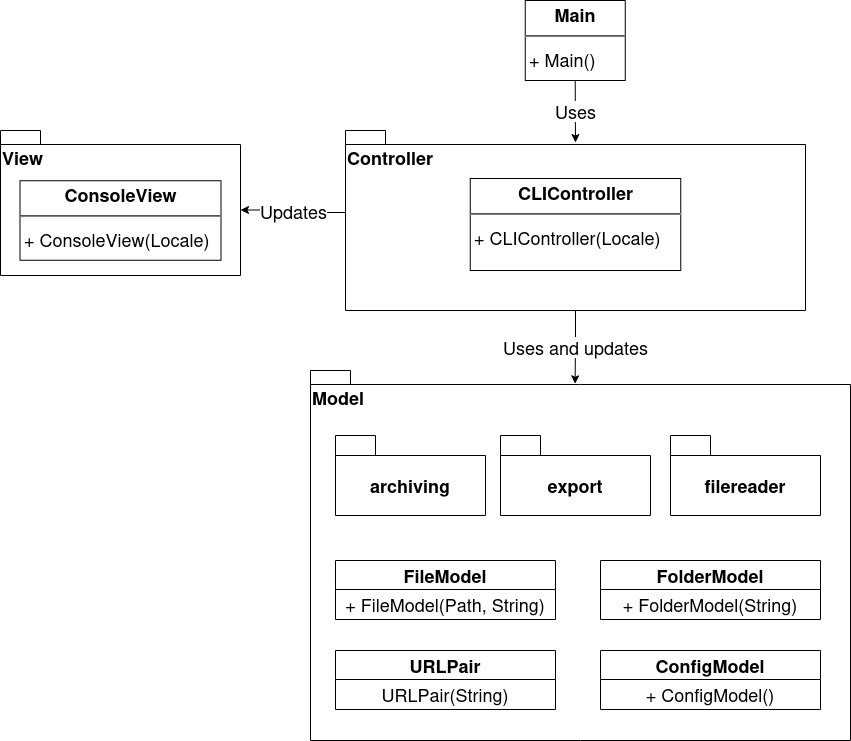
\includegraphics[width=0.7\textwidth]{diagrams/mvc_diagram-Highlevel_MVC.png}
    \caption{Highlevel Diagram of implemented MVC Pattern}
    \label{fig:MVC_Highlevel}
\end{figure}

\clearpage

\subsubsection{Factory Pattern}
The URL-Archiver makes extensive use of the Factory Pattern in its architecture, a key strategy in software engineering recognised for its role in the creational design paradigm. This pattern is central to the encapsulation of the object instantiation process. Rather than creating objects directly using the "new" operator, the Factory Pattern specifies a factory for this purpose. This abstraction improves the flexibility and scalability of the code.

The factory pattern is particularly useful when dealing with a variety of object types to be created, or when specific logic is required in their creation. Its implementation in the URL Archive provides a clear separation of concerns and improves code reusability, in line with the core principles of object-oriented design and programming.

In the URL-Archiver, the Factory Pattern is implemented in several key areas:

\begin{itemize}
	\item \textbf{File Readers:} Streamlines the addition of more input file types, thanks to its capability to produce objects conforming to the \texttt{FileReaderInterface}. This factory is pivotal in handling diverse file types.
	\item \textbf{Archiving Services:} Adding an additional service is straightforward, enhancing the application's ability to integrate different web archiving services.
	\item \textbf{Selenium Web Drivers:} Supports the integration of additional browsers with ease, showcasing the pattern’s adaptability in browser interactions.
	\item \textbf{Export Functionality:} The pattern's application here simplifies the inclusion of support for various file types in the export functionality.
\end{itemize}

These factories contribute significantly to the modularity and extensibility of the URL Archive by encapsulating the creation logic of various components, thus promoting loose coupling and scalability. The alignment of these approaches with the principles of the Factory Design Pattern underscores the maintainability of the application and its adaptability to new file types and data export formats.

The application of the factory pattern in the URL Archive is illustrated in figures \ref{fig:FileReaderFactory_Diagram} and \ref{fig:ExporterFactory_Diagram}, which show the \texttt{FileReaderFactory} and \texttt{ExporterFactory} respectively. Similar design principles are applied to other factories within the application, ensuring a consistent and modular approach across all components.

\begin{figure}[h!]
    \center
    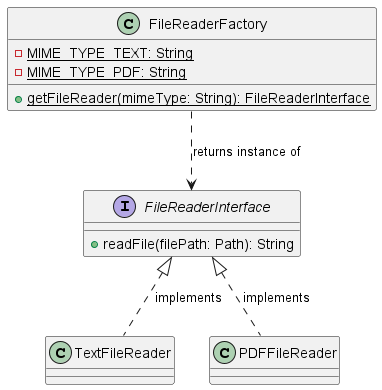
\includegraphics[width=0.5\textwidth]{pictures/FileReaderFactory-0.png}
    \caption{Diagram of the FileReader Factory}
    \label{fig:FileReaderFactory_Diagram}
\end{figure}

\begin{figure}[h!]
    \center
    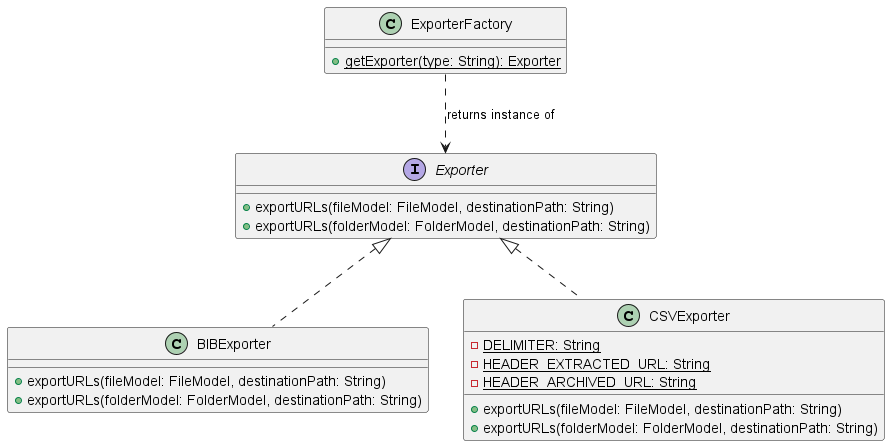
\includegraphics[width=0.9\textwidth]{pictures/ExporterFactory-0.png}
    \caption{Diagram of the Exporter Factory}
    \label{fig:ExporterFactory_Diagram}
\end{figure}

\subsubsection{Configuration File Management}
The URL-Archiver uses a JSON configuration file to effectively manage various settings and parameters. Key classes such as \texttt{ConfigModel} and \texttt{ConfigFileHelper} are integral to this process. The \texttt{ConfigModel} is used to define the structure of the configuration data, ensuring that all essential settings are systematically represented and easily accessible within the application. Conversely, the ConfigFileHelper is responsible for reading and writing the JSON configuration file, decoupling these tasks from the rest of the application code. This methodology not only streamlines the management of configuration settings, but also increases the adaptability of the application, as configuration changes do not require codebase changes.

An example of the configuration file structure is as follows:

\{

\quad''accessKey'':''[Access Key]'',

\quad''secretKey'':''[Secretkey]'',

\quad''browser'':''FIREFOX''

\}

Users have the flexibility to modify the configuration file at runtime, or edit the file directly. Currently, the application uses this file to store credentials for the Wayback Machine and to select the correct browser for the Archive Today service. This feature underlines the URL-Archiver's commitment to user customisation and operational efficiency.

\subsubsection{Adherence to SOLID Principles}
The URL-Archiver has been carefully designed with a strong emphasis on SOLID principles, ensuring a robust, maintainable and scalable architecture.

\begin{enumerate}
	\item \textbf{Single Responsibility Principle:} Each class, such as \texttt{FileReaderFactory}, \texttt{ConfigModel} or \texttt{CLIController}, is dedicated to a single responsibility. This principle ensures that each module or class focuses on a single aspect of the application's functionality.
	\item \textbf{Open/Closed Principle:} The application uses interfaces such as \texttt{FileReaderInterface} and factory classes to facilitate extensibility while keeping changes to existing code to a minimum. This approach allows new functionality to be added seamlessly.
	\item \textbf{Liskov Substitution Principle:} The architectural design allows subclasses (such as specific file readers) to replace their parent class or interface without compromising the integrity of the application, thereby maintaining a robust design.
	\item \textbf{Interface separation principle:} The design strategy of the URL Archive favours lean interfaces, ensuring that classes implement only the methods essential to their functionality. This is evident in the focused methods of interfaces such as \texttt{URLArchiver} and \texttt{Exporter}.
	\item \textbf{Dependency Inversion Principle:} High-level modules such as \texttt{CLIController} rely on abstractions rather than concrete implementations. This is emphasised by the use of interfaces and factory classes for object creation, which reduces dependency on specific implementations.
\end{enumerate}

The URL-Archiver's strict adherence to these SOLID principles is a testament to its well-structured, easily maintainable and scalable design. This approach underlines the application's commitment to high quality software engineering practices.

\subsubsection{Class Diagram}
Below the complete class diagram of this application is displayed. 

\clearpage

%\addcontentsline{lof}{figure}{UML Class Diagram URL-Archiver}
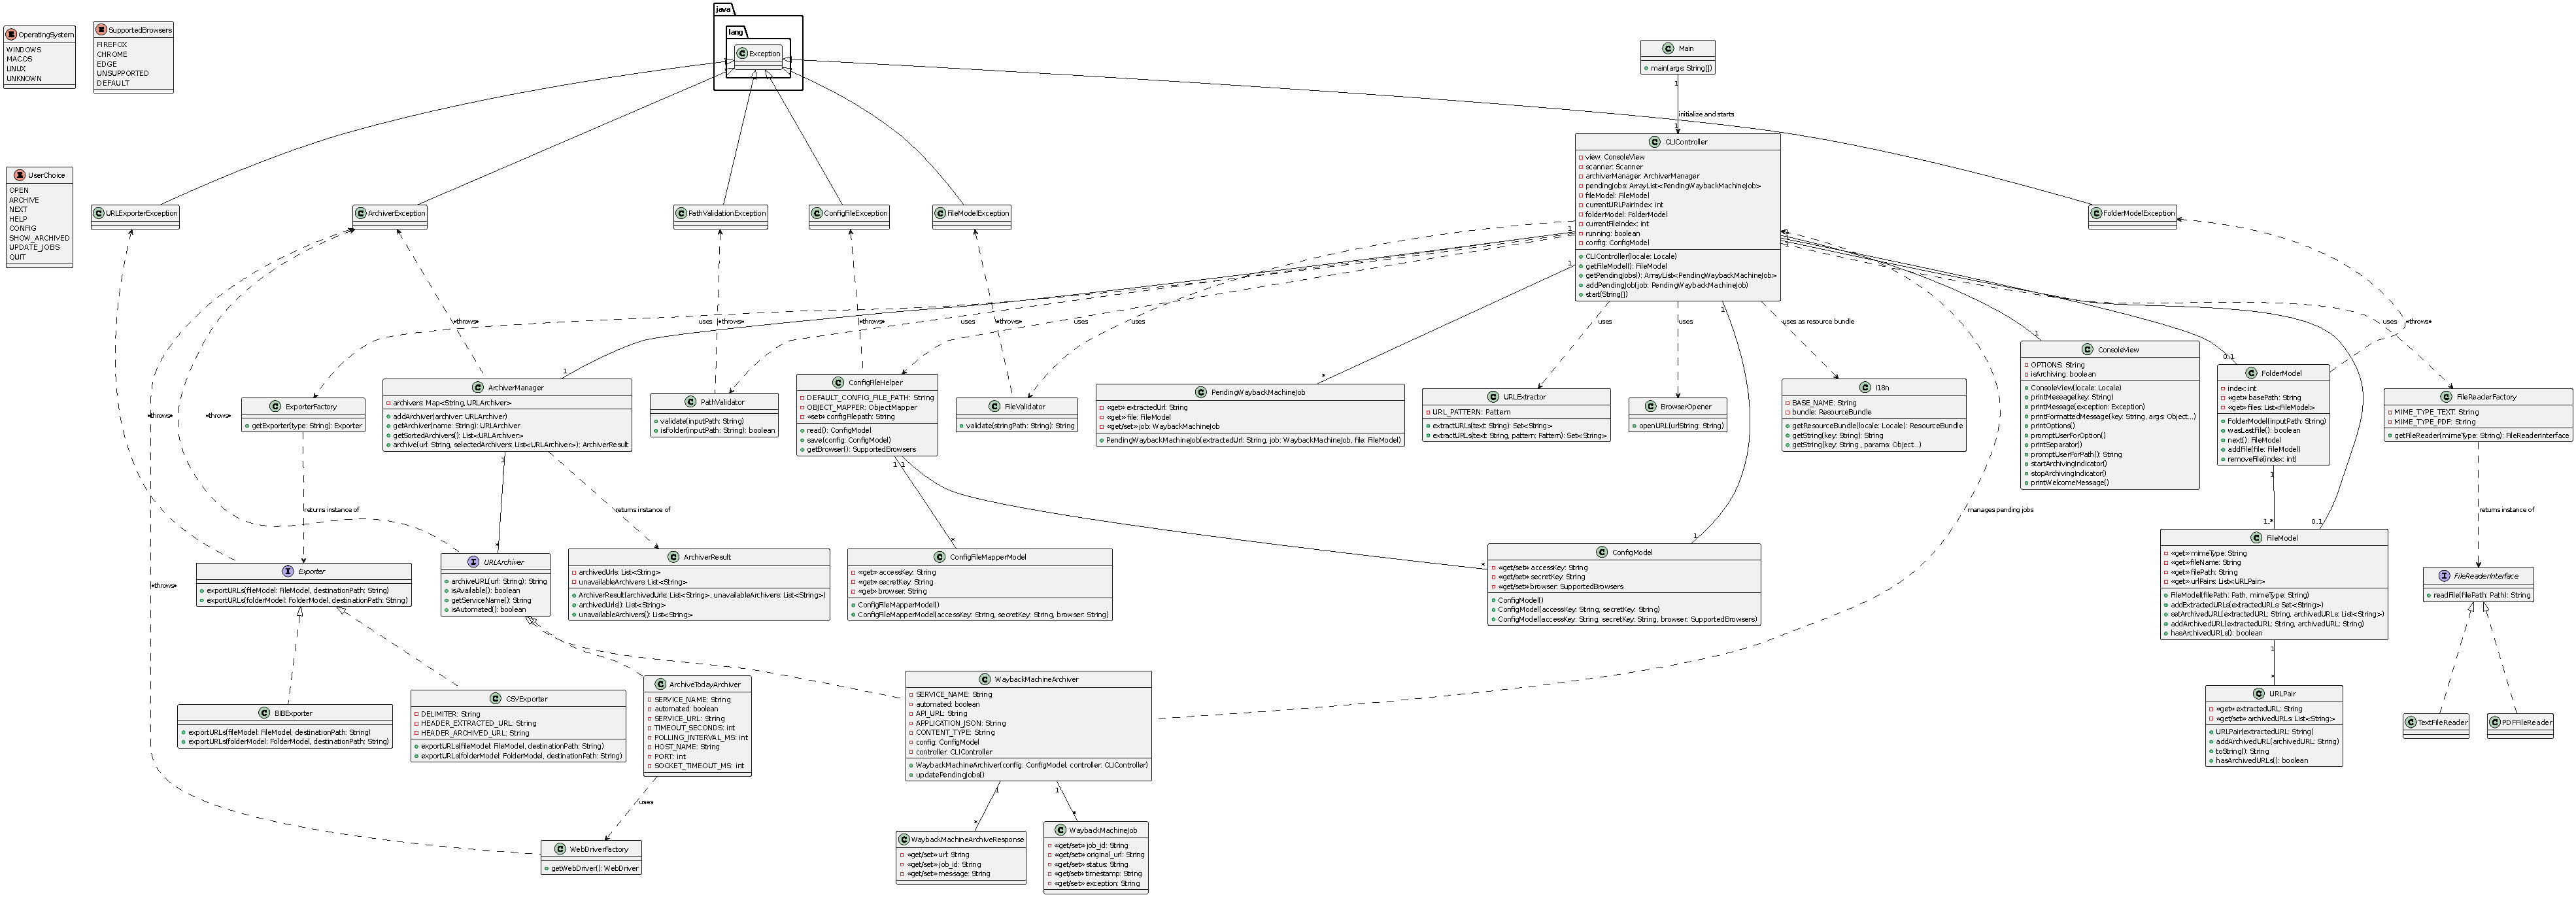
\includepdf[pages=1,fitpaper]{diagrams/uml_diagram.pdf}


\section{Processes}
% https://www.ganttlab.com
%					https://www.hermes.admin.ch/de/projektmanagement/verstehen/ubersicht-hermes/methodenubersicht.html

\subsection{Scrum}
We implemented our project utilizing the Scrum framework.
Over the course of the project, we completed six sprints.
Within these sprints, we tackled seven Epics, and successfully completed a total of 54 User Stories.
The progression of our project, along with the milestones and deliverables achieved, is illustrated in the subsequent Gantt chart.


\subsection{Allocation of roles}
In this chapter, the Scrum roles (Product Owner, Scrum Master, Developer) and additional roles such as Customer, Stakeholder, etc. are defined.


\subsection{Scrum roles}
We have decided to structure our Scrum team in the following manner:
\begin{table}[ht]
    \centering
    \begin{bfhTabular}{lll}
        \textbf{Role} & \textbf{Person}\\\hline
        Product Owner & Nicolin Dora\\\hline
        Scrum Master  & Abidin Vejseli\\\hline
        Developer     & Nicolin Dora, Abidin Vejseli, Kilian Wampfler\\\hline
    \end{bfhTabular}
    \caption{Scrum Roles}
    \label{tab:tab1}
\end{table}

Nicolin took on the role of Product Owner as he had concrete ideas and visions for the product at the start of the project.
Additionally, he took on this role because he wanted to deal with the subjects surrounding the product backlog.

Abidin took on the role of the Scrum Master as he has the most experience with the agile way of working.
He has already had the opportunity to perform this role professionally on several smaller projects in the past.

Kilian took on the role of a Developer, as he is an active programmer in his job and has already gained some experience with Scrum.
Therefore, self-organization is not a foreign concept to him.

Besides Kilian, all the other members of the group were also assigned the role of Developer, as otherwise the project would not have been feasible in the given time. This is due to the fact that we all work alongside the university.

\subsection{Additional roles}
In addition to the Scrum roles, we have assigned the following roles to our specialist lecturer and PM-coach.
\begin{table}[ht]
    \centering
    \begin{bfhTabular}{lll}
        \textbf{Role} & \textbf{Person}\\\hline
        Stakeholder   & Dr. Simon Kramer\\\hline
        Customer      & Dr. Simon Kramer\\\hline
        PM-Advisor    & Frank Helbling\\\hline
    \end{bfhTabular}
    \caption{Additional Scrum Roles}
    \label{tab:tab2}
\end{table}

\subsection{Scrum Adaptionen}
As part of Project 1, we have adjusted Scrum in order to use it in the best possible way.
The major adjustments are explained in this chapter.

\subsubsection{Definition of Ready (DOR)}
Our DOR includes conditions that ensure that all team members understand the user stories and know when a user story can be included in a sprint. The DOR was set in line with the INVEST\footnote{\href{https://xp123.com/articles/invest-in-good-stories-and-smart-tasks/}{XP123 article: Invest in good stories and smart tasks}} criteria. A user story in the product backlog must meet the DOR before it can be included in a sprint.

\textbf{Definition of Ready}
\begin{itemize}
    \item Ensure a clear definition
    \item Define the functionality or requirement to be implemented
    \item Clearly defined and testable acceptance criteria
    \item Ensure there are no or minimal dependencies
    \item Understood by the whole team
    \item The user story has been estimated
    \item The scope of the user story is small enough that it can be implemented in a single sprint.
\end{itemize}
\clearpage

\subsubsection{Definition of Done (DOD)}
Our DOD contains all the characteristics and standards that a user story must meet to be considered complete.
Once it satisfies the necessary quality requirements (acceptance criteria), the story can be considered complete and can be closed.
The goal of our DOD is to create transparency so that everyone has a common understanding of when a story can be closed.
A story that does not comply with the DOD may not be finalised.

\textbf{Definition of Done}
\begin{itemize}
    \item Coding standards and best practices are implemented
    \item Unit tests for the feature are written and passe
    \item Any changes to the code or functionality are documented
    \item The code and functionality are reviewed by peers
    \item The feature works across multiple platforms
    \item Code is integrated with master branch
    \item Documentation has been updated
    \item Acceptance criteria are met
\end{itemize}

\subsubsection{Sprint}
As a team, we have decided that our sprints will take place at two-week intervals.
For each sprint we define a SMART sprint goal, which specifies the relevant user stories.

We decided in favour of the two-week rhythm because regular feedback is important to us and thus creates a greater learning effect.
Additionally, we ascertained that one-week sprints would result in excessive overheads due to the administrative work involved in Scrum.
Likewise, we consider sprints longer than two weeks to be impractical, as the interaction would suffer.

\subsubsection{Daily Scrum}
As a team, we have decided not to have daily Scrum meetings, as this is not possible because all team members do work part times. Instead, we have two weekly meetings (weeklys), on Wednesday and Friday at 17:00, which last a maximum of 15 minutes.
In addition, we have chosen to hold the meetings through Microsoft Teams as it is easier to organise.
The goal of these meetings is to share the current progress, address issues, update the team and briefly discuss the next steps.
%\subsection{Allocation of roles}
In this chapter, the Scrum roles (Product Owner, Scrum Master, Developer) and additional roles such as Customer, Stakeholder, etc. are defined.


\subsection{Scrum roles}
We have decided to structure our Scrum team in the following manner:
\begin{table}[ht]
    \centering
    \begin{bfhTabular}{lll}
        \textbf{Role} & \textbf{Person}\\\hline
        Product Owner & Nicolin Dora\\\hline
        Scrum Master  & Abidin Vejseli\\\hline
        Developer     & Nicolin Dora, Abidin Vejseli, Kilian Wampfler\\\hline
    \end{bfhTabular}
    \caption{Scrum Roles}
    \label{tab:tab1}
\end{table}

Nicolin took on the role of Product Owner as he had concrete ideas and visions for the product at the start of the project.
Additionally, he took on this role because he wanted to deal with the subjects surrounding the product backlog.

Abidin took on the role of the Scrum Master as he has the most experience with the agile way of working.
He has already had the opportunity to perform this role professionally on several smaller projects in the past.

Kilian took on the role of a Developer, as he is an active programmer in his job and has already gained some experience with Scrum.
Therefore, self-organization is not a foreign concept to him.

Besides Kilian, all the other members of the group were also assigned the role of Developer, as otherwise the project would not have been feasible in the given time. This is due to the fact that we all work alongside the university.


\subsection{Additional roles}
In addition to the Scrum roles, we have assigned the following roles to our specialist lecturer and PM-coach.
\begin{table}[ht]
    \centering
    \begin{bfhTabular}{lll}
        \textbf{Role} & \textbf{Person}\\\hline
        Stakeholder   & Dr. Simon Kramer\\\hline
        Customer      & Dr. Simon Kramer\\\hline
        PM-Advisor    & Frank Helbling\\\hline
    \end{bfhTabular}
    \caption{Additional Scrum Roles}
    \label{tab:tab2}
\end{table}


\subsection{Sprint Goals}
We have defined the goals of our past and current sprints in the best possible way according to the SMART\footnote{\href{https://www.atlassian.com/blog/productivity/how-to-write-smart-goals}{Atlassian blogpost: "How to write smart goals"}} criteria. The goals of our sprints are listed below:

\paragraph{Sprint 1}
Implement input handler for files (any unicode file e.g. .bib, .txt, .html and .pdf) and basic user guidance (Menu, Error messages).

\paragraph{Sprint 2}
Implement a function to scan a provided text in order to identify and extract any URLs contained within it and upgrade our current console-based interface to enable users to easily open any extracted URL using their default web browser.

\paragraph{Sprint 3}
Develop and implement a fully automated URL submission system that integrates with the Wayback Machine and Archive Today to ensure at least a 98% success rate in URL archiving.

\paragraph{Sprint 4}
Enhance the system's stability and usability by resolving identified Selenium bugs across Linux, macOS, and Edge browsers, documenting the sprint process and licenses, conducting a thorough code review, and establishing a new configuration management file, aiming for zero critical bugs at sprint closure and readying the system for seamless URL archiving integration in subsequent sprints.

\paragraph{Sprint 5}
Complete application refactoring for asynchronous archiving and .BIB file URL integration, ensuring no critical bugs and preparing for seamless future enhancements.

\paragraph{Sprint 6}
Deliver a finalized application design, improved code quality, and complete documentation, with all components ready for review.

\clearpage

\subsection{Requirements}
In this chapter, we present our product and sprint backlogs, structured according to Scrum.

\subsubsection{Product Backlog}
Our product backlog consists of user stories and epics created by our Product Owner.
The user stories are prioritised and represent a set of initial requirements that must be met to achieve our product goal. The product backlog is maintained in Jira.
\begin{figure}[h!]
    \centering
    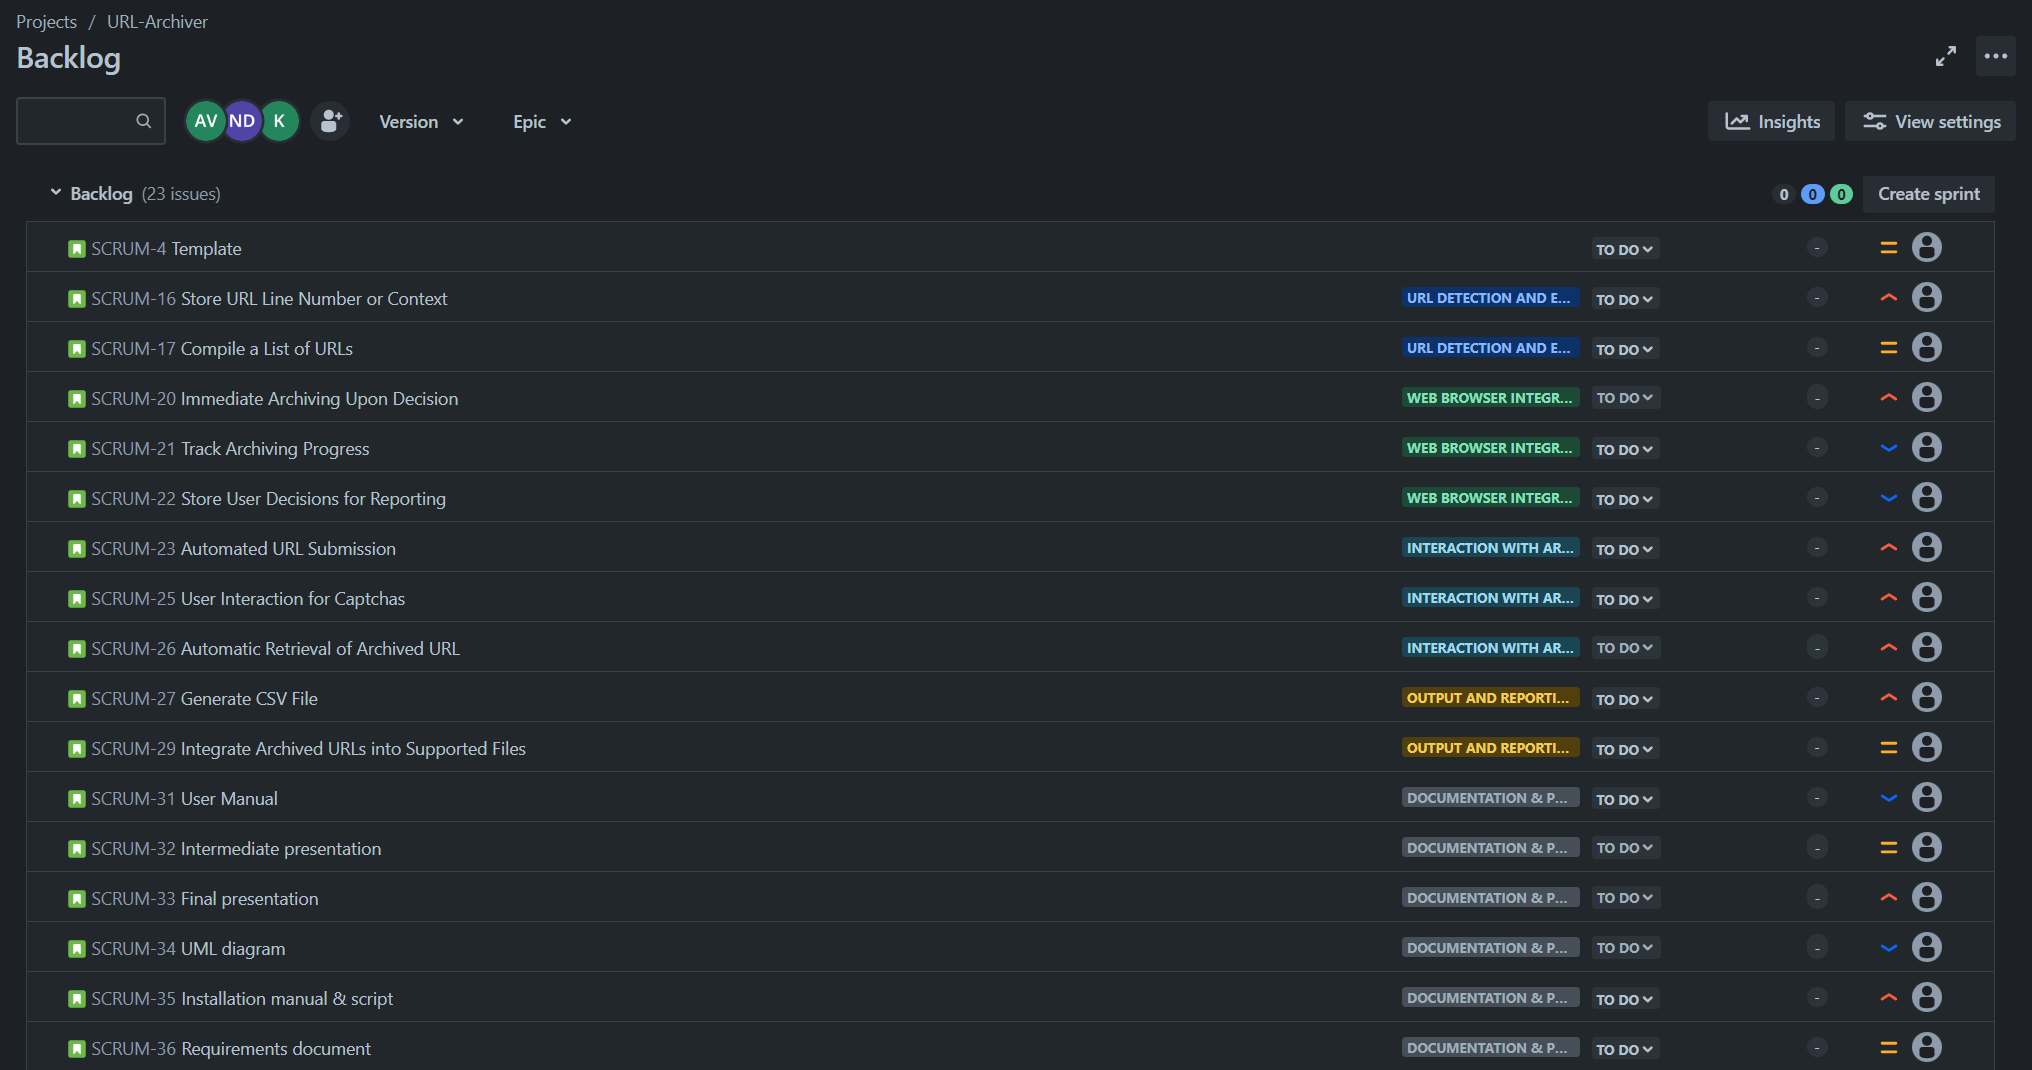
\includegraphics[width=1\textwidth]{pictures/backlog}
    \caption{Product Backlog}
    \label{fig:backlog}
\end{figure}

The prioritisation of user stories in the backlog is based on the business value field, which has a value between one and ten.
The business value is a vague estimate of how much value the individual user story has to the business, or in our case, to our stakeholders.
We endeavour to estimate the business value based on the expected importance of the function to the stakeholder.
The following priorities are possible:
\begin{itemize}
    \item Highest
    \item High
    \item Medium
    \item Low
    \item Lowest
\end{itemize}

\subsubsection{Sprint Backlogs}
Below we describe our recent and current sprints.
During the sprint planning we fill the respective sprint backlog with user stories that serve the sprint goal.
A user story must satisfy our Definition of Ready before it can be included in the sprint.
In addition, the stories must be estimated and the total number of story points must not exceed our defined velocity.

\paragraph{Sprint 1}
Below is a screenshot of our board from the first sprint with the corresponding sprint goal.
\begin{figure}[h!]
    \centering
    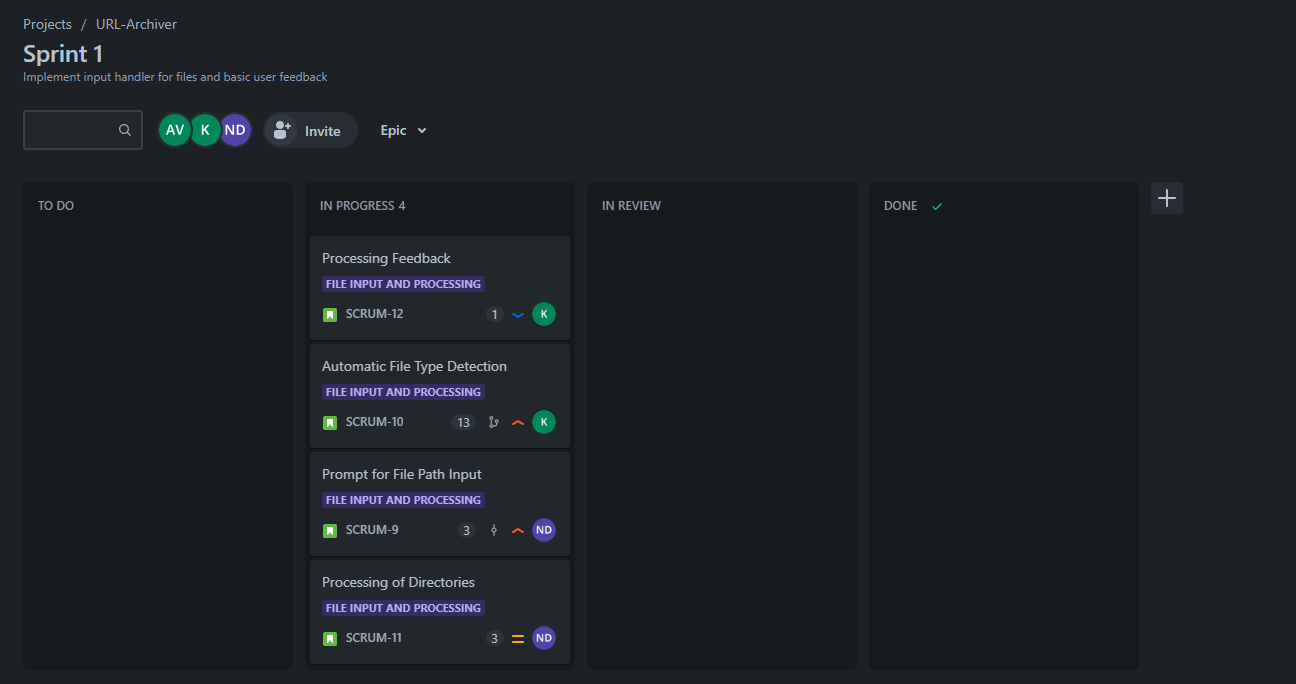
\includegraphics[width=1\textwidth]{pictures/backlog_sprint_1}
    \caption{Sprint 1 Backlog}
    \label{fig:backlog_sprint_1}
\end{figure}

The user stories from the first sprint are shown below. The stories have been estimated and prioritised.

\begin{figure}[h!]
    \centering
    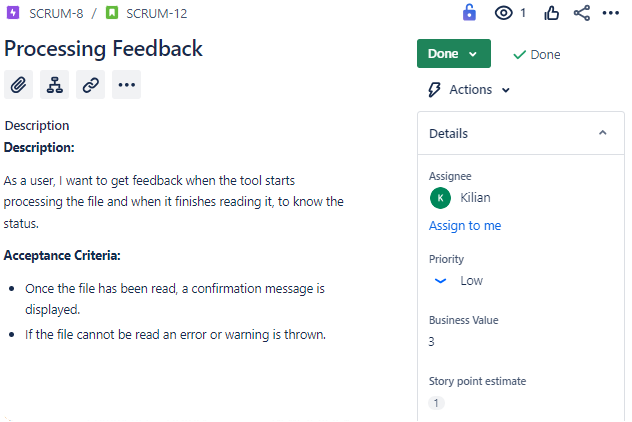
\includegraphics[width=1\textwidth]{pictures/Scrum/Sprint 1/UserStory_4}
    \caption{User Story Detail for "Processing Feedback"}
    \label{fig:sprint_1_userstory_1}
\end{figure}
\begin{figure}[h!]
    \centering
    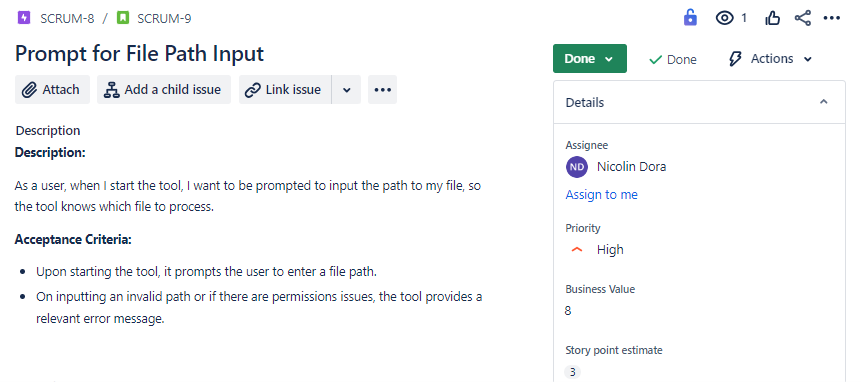
\includegraphics[width=1\textwidth]{pictures/Scrum/Sprint 1/UserStory_1}
    \caption{User Story Detail for "Prompt for file path input"}
    \label{fig:sprint_1_userstory_2}
\end{figure}
\begin{figure}[h!]
    \centering
    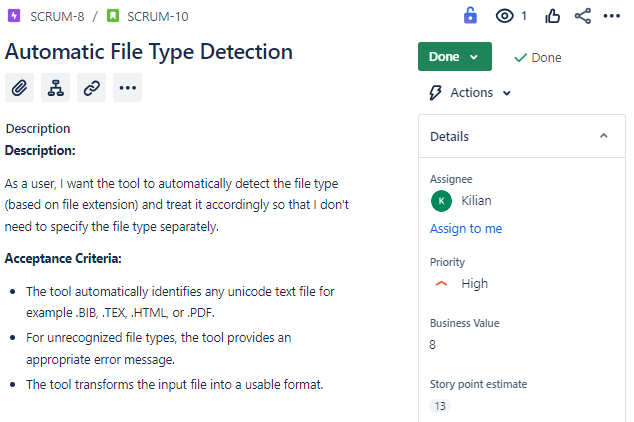
\includegraphics[width=1\textwidth]{pictures/Scrum/Sprint 1/UserStory_2}
    \caption{User Story Detail for "Automatic File Type Detection"}
    \label{fig:sprint_1_userstory_3}
\end{figure}
\begin{figure}[h!]
    \centering
    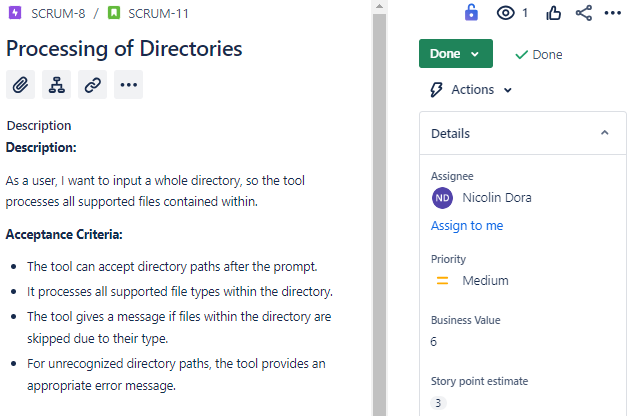
\includegraphics[width=1\textwidth]{pictures/Scrum/Sprint 1/UserStory_3}
    \caption{User Story Detail for "Processing of Directories"}
    \label{fig:sprint_1_userstory_4}
\end{figure}
\clearpage

In the first sprint, the burn down chart looks like this:
\begin{figure}[h!]
    \centering
    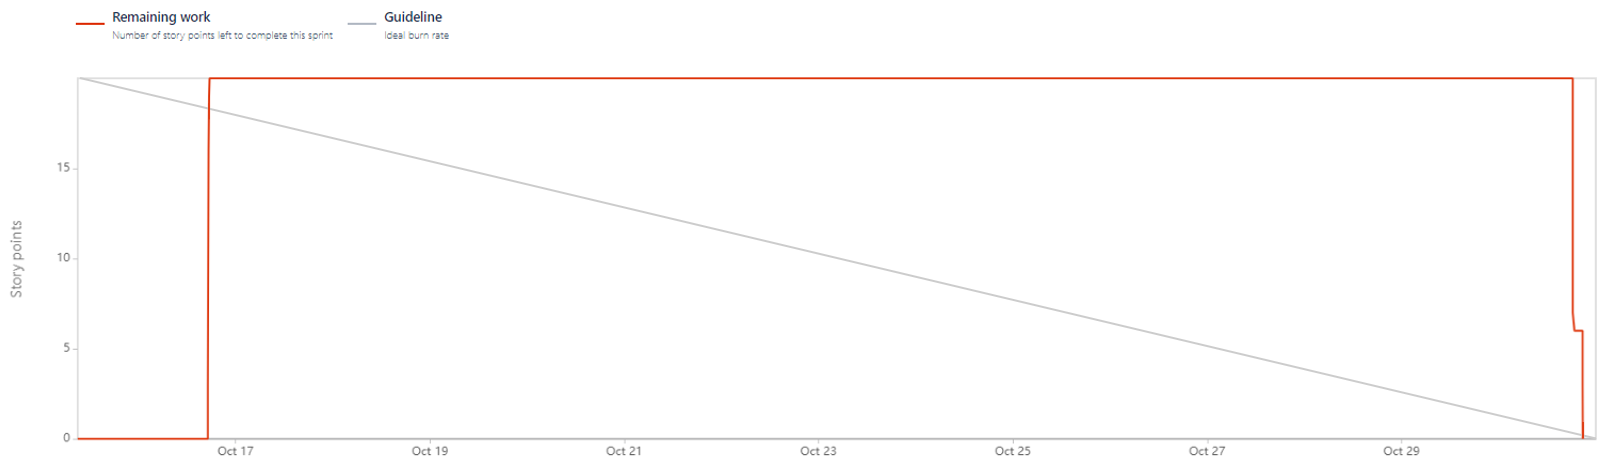
\includegraphics[width=1\textwidth]{pictures/Scrum/Sprint 1/sprint1_burndownchart}
    \caption{Sprint 1 Burn Up Chart}
    \label{fig:sprint_1_bunrdown_chart}
\end{figure}

The reason for this is that we did not create tasks for our user stories as they were small enough.
Furthermore, a code review for corresponding user stories could only be conducted towards the end of the sprint, resulting in the finalisation of user stories at that point.
\clearpage

\paragraph{Sprint 2}
Below is a screenshot of our board from the second sprint with the corresponding sprint goal.
\begin{figure}[h!]
    \centering
    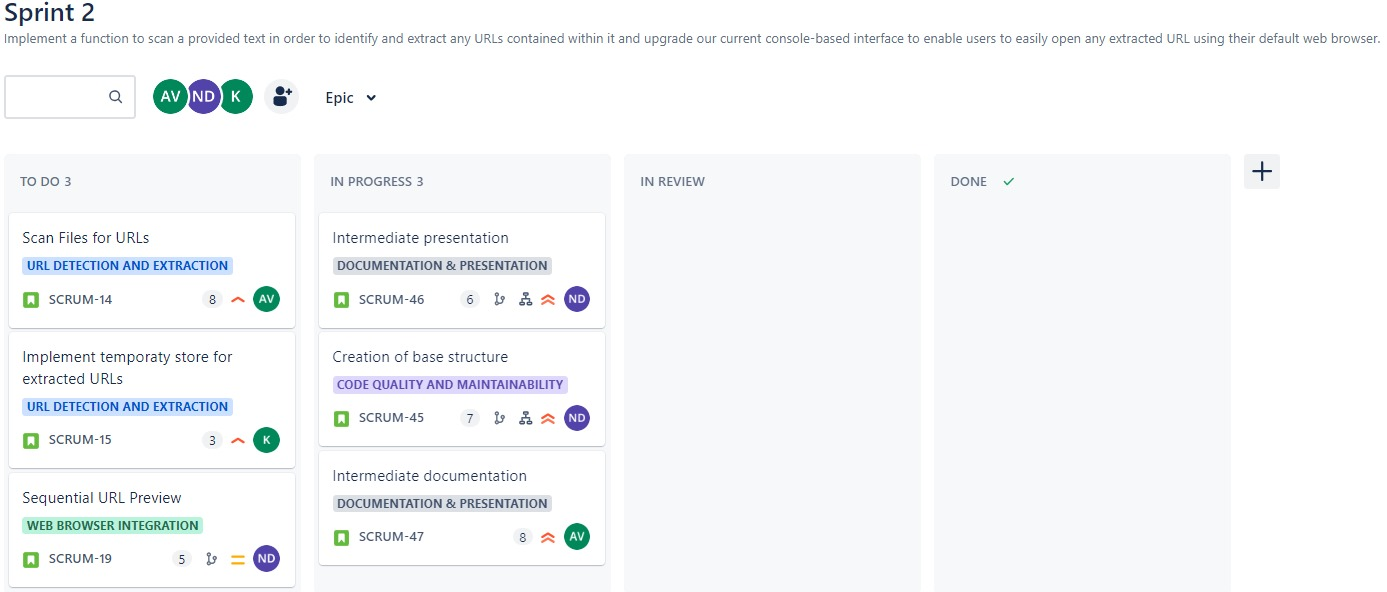
\includegraphics[width=1\textwidth]{pictures/Scrum/Sprint 2/Sprint2_Backlog}
    \caption{Sprint 2 Backlog}
    \label{fig:sprint_2_backlog}
\end{figure}

The user stories from the second sprint are shown below. The stories have been estimated and prioritised.
\begin{figure}[h!]
    \centering
    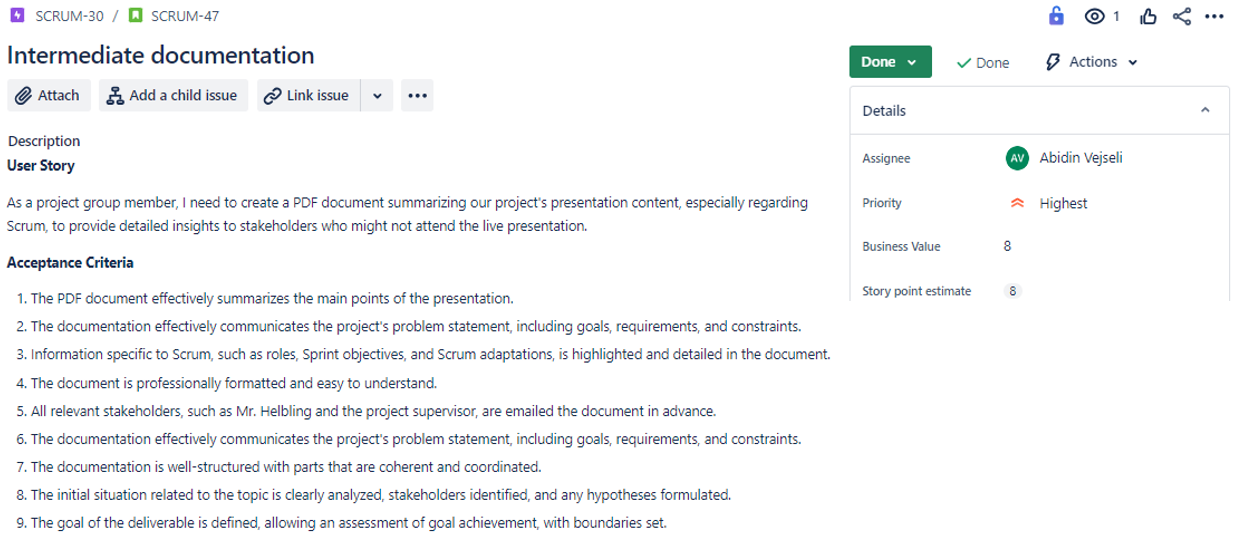
\includegraphics[width=1\textwidth]{pictures/Scrum/Sprint 2/UserStory_13}
    \caption{User Story Detail for "Intermediate Documentation"}
    \label{fig:sprint_2_userstory_1}
\end{figure}
\begin{figure}[h!]
    \centering
    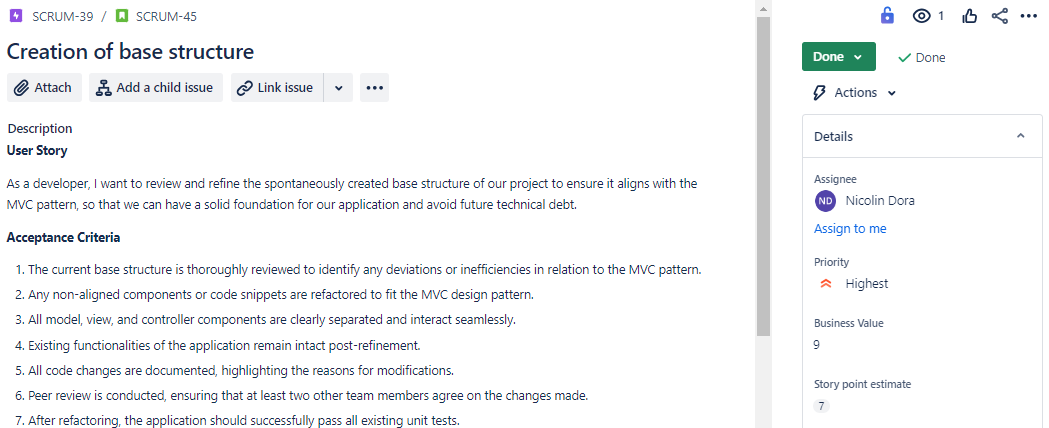
\includegraphics[width=1\textwidth]{pictures/Scrum/Sprint 2/UserStory_11}
    \caption{User Story Detail for "Creation of Base Structure"}
    \label{fig:sprint_2_userstory_2}
\end{figure}
\begin{figure}[h!]
    \centering
    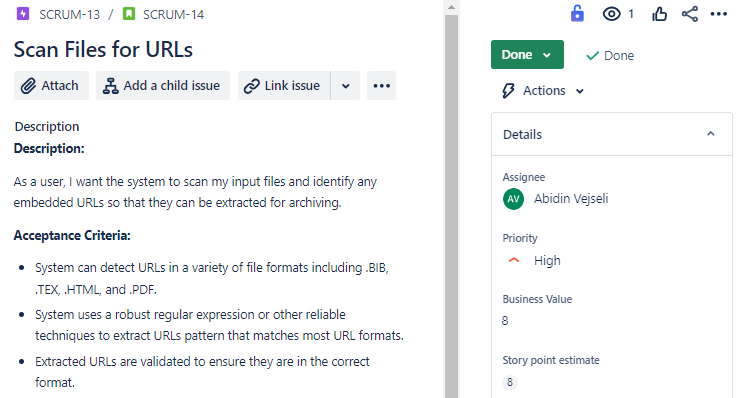
\includegraphics[width=1\textwidth]{pictures/Scrum/Sprint 2/UserStory_5}
    \caption{User Story Detail for "Scan Files for URLs"}
    \label{fig:sprint_2_userstory_3}
\end{figure}
\begin{figure}[h!]
    \centering
    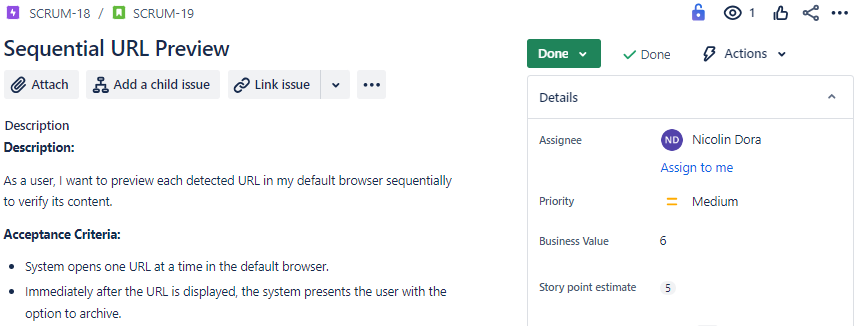
\includegraphics[width=1\textwidth]{pictures/Scrum/Sprint 2/UserStory_7}
    \caption{User Story Detail for "Sequential URL Preview"}
    \label{fig:sprint_2_userstory_4}
\end{figure}
\begin{figure}[h!]
    \centering
    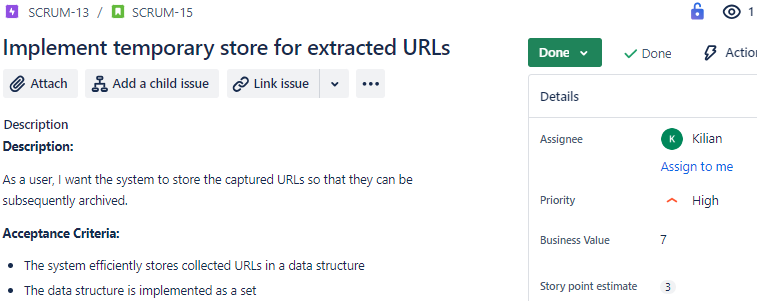
\includegraphics[width=1\textwidth]{pictures/Scrum/Sprint 2/UserStory_6}
    \caption{User Story Detail for "Implement temporary store for extracted URLs"}
    \label{fig:sprint_2_userstory_5}
\end{figure}
\begin{figure}[h!]
    \centering
    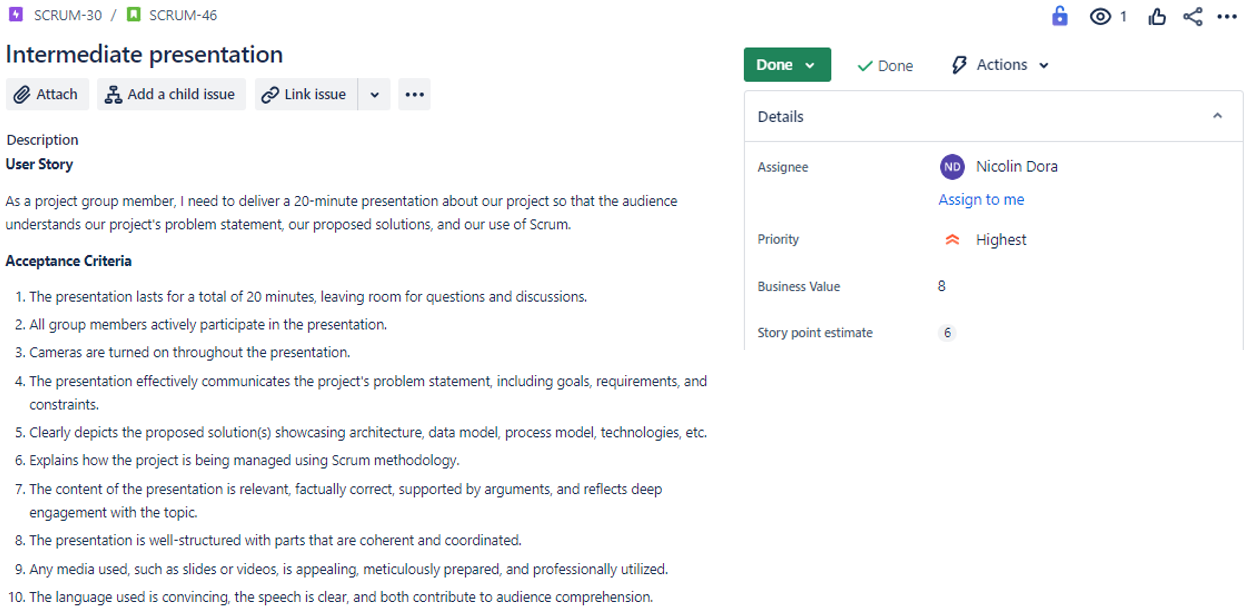
\includegraphics[width=1\textwidth]{pictures/Scrum/Sprint 2/UserStory_12}
    \caption{User Story Detail for "Intermediate presentation"}
    \label{fig:sprint_2_userstory_6}
\end{figure}
\clearpage

In the second sprint, the burn down chart looks like this:
\begin{figure}[h!]
    \centering
    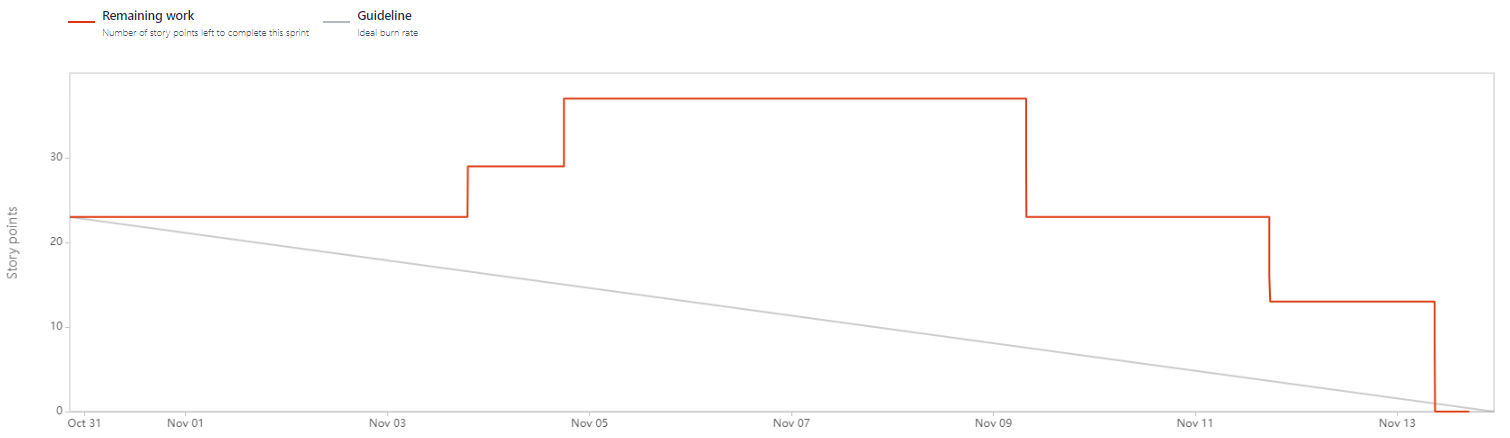
\includegraphics[width=1\textwidth]{pictures/Scrum/Sprint 2/Sprint2_burndownchart}
    \caption{Sprint 2 Burn Down Chart}
    \label{fig:sprint_2_bunrdown_chart}
\end{figure}

Compared to the initial sprint, our workload significantly increased, and we introduced new user stories after the sprint began.
Despite these additions, we maintained a strong pace and seamlessly managed the extra tasks that arose from the intermediate presentation and documentation requirements.
\clearpage


\paragraph{Sprint 3}
Below is a screenshot of our board from the third sprint with the corresponding sprint goal.
\begin{figure}[h!]
    \centering
    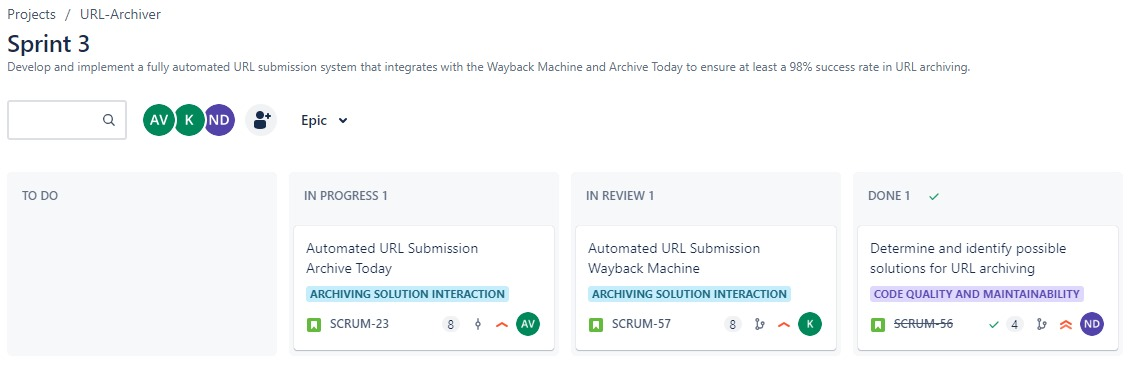
\includegraphics[width=1\textwidth]{pictures/Scrum/Sprint 3/Sprint3_Backlog}
    \caption{Sprint 3 Backlog}
    \label{fig:sprint_3_backlog}
\end{figure}

The user stories from the third sprint are shown below. The stories have been estimated and prioritised.
\begin{figure}[h!]
    \centering
    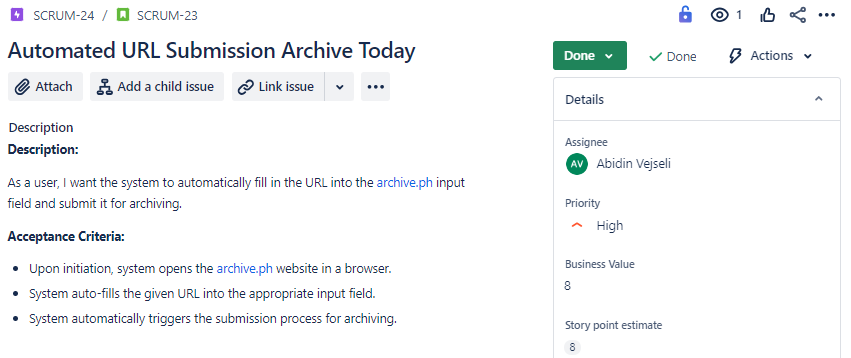
\includegraphics[width=1\textwidth]{pictures/Scrum/Sprint 3/UserStory_8}
    \caption{User Story Detail for "Intermediate Documentation"}
    \label{fig:sprint_3_userstory_1}
\end{figure}
\begin{figure}[h!]
    \centering
    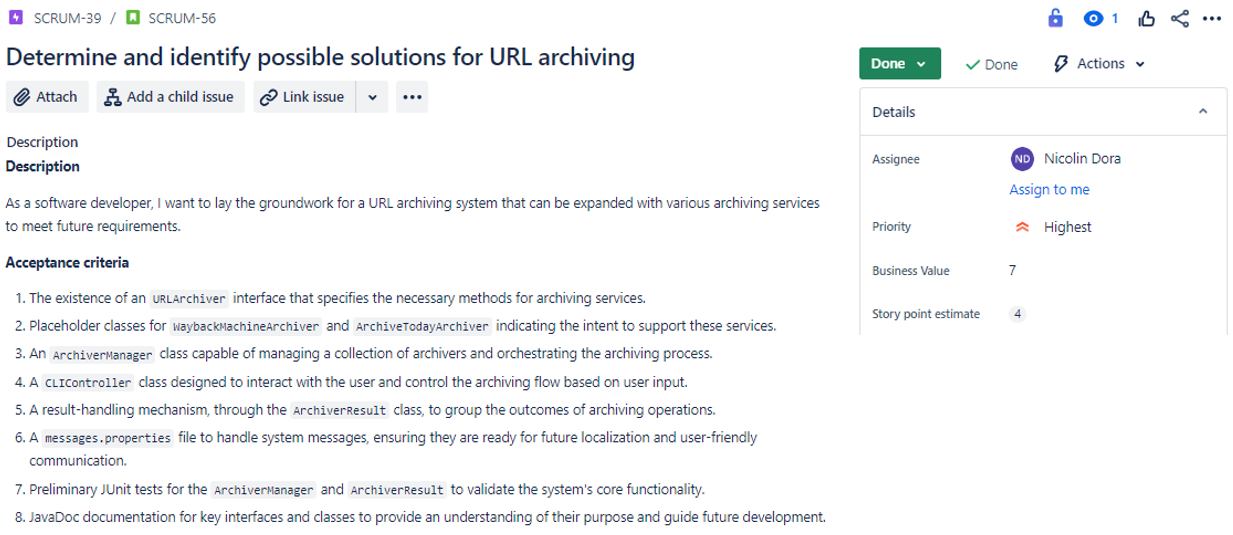
\includegraphics[width=1\textwidth]{pictures/Scrum/Sprint 3/UserStory_14}
    \caption{User Story Detail for "Creation of Base Structure"}
    \label{fig:sprint_3_userstory_2}
\end{figure}
\begin{figure}[h!]
    \centering
    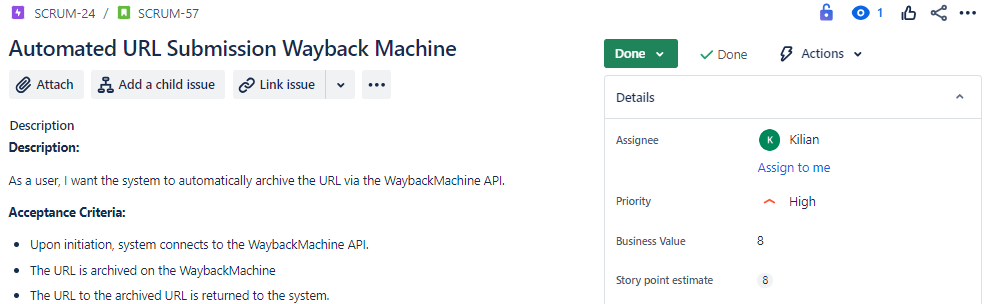
\includegraphics[width=1\textwidth]{pictures/Scrum/Sprint 3/UserStory_15}
    \caption{User Story Detail for "Scan Files for URLs"}
    \label{fig:sprint_3_userstory_3}
\end{figure}

In the third sprint, the burn down chart looks like this:
\begin{figure}[h!]
    \centering
    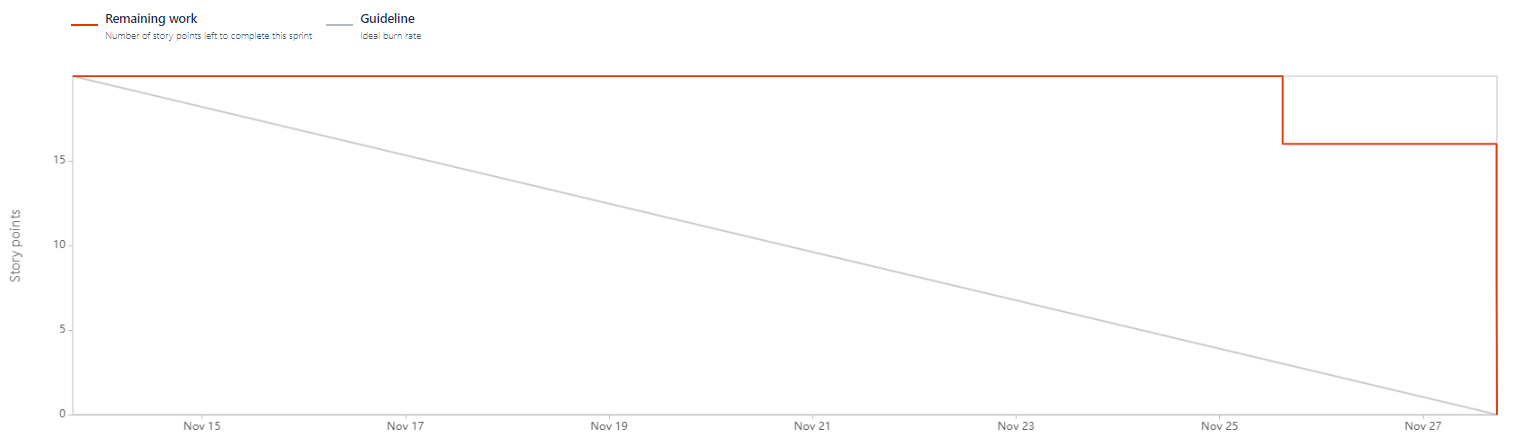
\includegraphics[width=1\textwidth]{pictures/Scrum/Sprint 3/Sprint3_burndownchart}
    \caption{Sprint 3 Burn Down Chart}
    \label{fig:sprint_3_bunrdown_chart}
\end{figure}

During the third sprint, our progress on user stories was limited to the completion of only three due to the 'special week 3'.
This meant that these stories had to be completed in the second half of the sprint due to the heavy workload of this special week.
The impact of this adaptation to our sprint schedule due to 'special week 3' is reflected in the trends seen in our burndown chart.
\clearpage

\paragraph{Sprint 4}
Below is a screenshot of our board from the forth sprint.
\begin{figure}[h!]
    \centering
    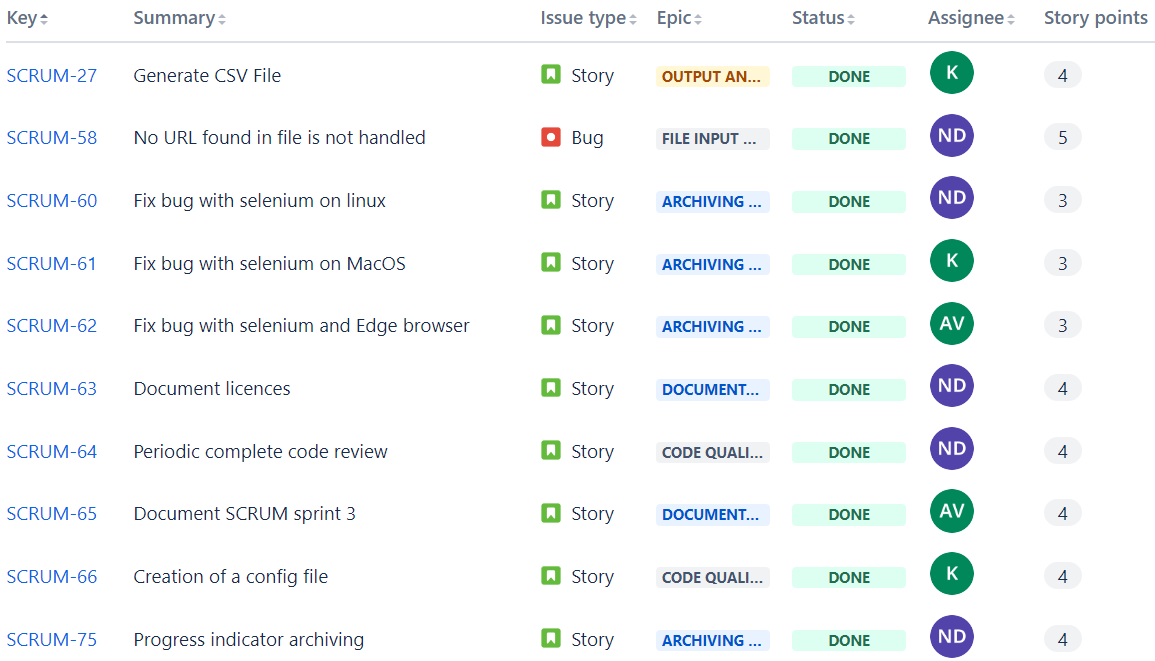
\includegraphics[width=1\textwidth]{pictures/Scrum/Sprint 4/Sprint4_Backlog}
    \caption{Sprint 4 Backlog}
    \label{fig:sprint_4_backlog}
\end{figure}

The user stories from the forth sprint are shown below. The stories have been estimated and prioritised.
\begin{figure}[h!]
    \centering
    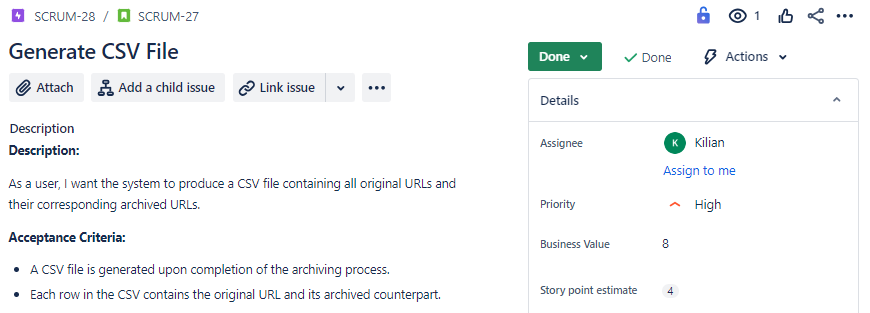
\includegraphics[width=1\textwidth]{pictures/Scrum/Sprint 4/UserStory_9}
    \caption{User Story Detail for "Generate CSV File"}
    \label{fig:sprint_4_userstory_1}
\end{figure}
\begin{figure}[h!]
    \centering
    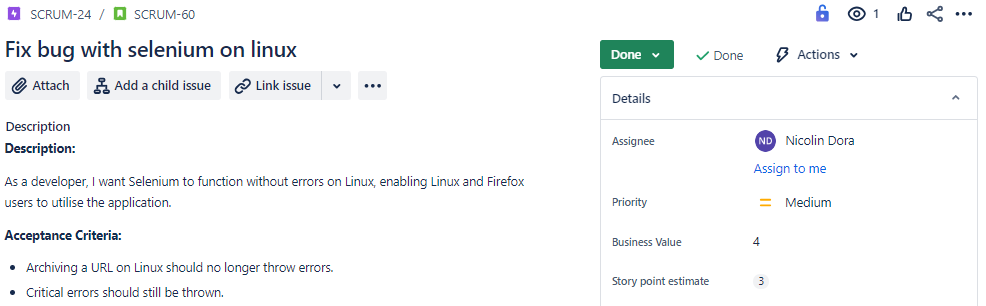
\includegraphics[width=1\textwidth]{pictures/Scrum/Sprint 4/UserStory_16}
    \caption{User Story Detail for "Fix bug with selenium on linux"}
    \label{fig:sprint_4_userstory_2}
\end{figure}
\begin{figure}[h!]
    \centering
    \includegraphics[width=1\textwidth]{pictures/Scrum/Sprint 4/UserStory_17}
    \caption{User Story Detail for "Fix bug with selenium on MacOS"}
    \label{fig:sprint_4_userstory_3}
\end{figure}
\begin{figure}[h!]
    \centering
    \includegraphics[width=1\textwidth]{pictures/Scrum/Sprint 4/UserStory_18}
    \caption{User Story Detail for "Fix bug With selenium and Edge browser"}
    \label{fig:sprint_4_userstory_4}
\end{figure}
\begin{figure}[h!]
    \centering
    \includegraphics[width=1\textwidth]{pictures/Scrum/Sprint 4/UserStory_19}
    \caption{User Story Detail for "Document licences"}
    \label{fig:sprint_4_userstory_5}
\end{figure}
\begin{figure}[h!]
    \centering
    \includegraphics[width=1\textwidth]{pictures/Scrum/Sprint 4/UserStory_20}
    \caption{User Story Detail for "Periodic complete code review"}
    \label{fig:sprint_4_userstory_6}
\end{figure}
\begin{figure}[h!]
    \centering
    \includegraphics[width=1\textwidth]{pictures/Scrum/Sprint 4/UserStory_21}
    \caption{User Story Detail for "Document SCRUM sprint 3"}
    \label{fig:sprint_4_userstory_7}
\end{figure}
\begin{figure}[h!]
    \centering
    \includegraphics[width=1\textwidth]{pictures/Scrum/Sprint 4/UserStory_22}
    \caption{User Story Detail for "Creation of a config file"}
    \label{fig:sprint_4_userstory_8}
\end{figure}
\begin{figure}[h!]
    \centering
    \includegraphics[width=1\textwidth]{pictures/Scrum/Sprint 4/UserStory_24}
    \caption{User Story Detail for "Progress indicator archiving"}
    \label{fig:sprint_4_userstory_9}
\end{figure}
\begin{figure}[h!]
    \centering
    \includegraphics[width=1\textwidth]{pictures/Scrum/Sprint 4/Bug_1}
    \caption{Bug Detail for "No URL found in file is not handled"}
    \label{fig:sprint_4_bug_1}
\end{figure}


In the forth sprint, the burn down chart looks like this:
\begin{figure}[h!]
    \centering
    \includegraphics[width=1\textwidth]{pictures/Scrum/Sprint 4/Sprint4_Burndownchart}
    \caption{Sprint 4 Burn Down Chart}
    \label{fig:sprint_4_bunrdown_chart}
\end{figure}

Compared to the previous sprint, we were more efficient and successfully accommodated additional user stories that were initiated after the sprint began.
The completion of all allocated user stories within the sprint timeframe demonstrates our solid teamwork and sprint management capabilities.
\clearpage


\paragraph{Sprint 5}
Below is a screenshot of our board from the fifth sprint.
\begin{figure}[h!]
    \centering
    \includegraphics[width=1\textwidth]{pictures/Scrum/Sprint 5/Sprint5_Backlog}
    \caption{Sprint 5 Backlog}
    \label{fig:sprint_5_backlog}
\end{figure}

The user stories from the fifth sprint are shown below. The stories have been estimated and prioritised.
\begin{figure}[h!]
    \centering
    \includegraphics[width=1\textwidth]{pictures/Scrum/Sprint 5/UserStory_10}
    \caption{User Story Detail for "Integrate Archived URLs into Supported Files"}
    \label{fig:sprint_5_userstory_1}
\end{figure}
\begin{figure}[h!]
    \centering
    \includegraphics[width=1\textwidth]{pictures/Scrum/Sprint 5/UserStory_23}
    \caption{User Story Detail for "Create / Fix Tests"}
    \label{fig:sprint_5_userstory_2}
\end{figure}
\begin{figure}[h!]
    \centering
    \includegraphics[width=1\textwidth]{pictures/Scrum/Sprint 5/UserStory_25}
    \caption{User Story Detail for "Show archived urls path"}
    \label{fig:sprint_5_userstory_3}
\end{figure}

In the fifth sprint, the burn down chart looks like this:
\begin{figure}[h!]
    \centering
    \includegraphics[width=1\textwidth]{pictures/Scrum/Sprint 5/Sprint5_Burndownchart}
    \caption{Sprint 5 Burn Down Chart}
    \label{fig:sprint_5_bunrdown_chart}
\end{figure}

In sprint 5, our time was limited due to commitments in other modules and the upcoming Christmas period, which resulted in team member absences.
We encountered an unexpected challenge with the extensive time required for test refactoring, as we prioritise quality, which often demands more time.
As a result, we were unable to complete all planned user stories and had to carry them over to the next sprint.
These challenges are reflected in the burn down chart.
\clearpage


\subsection{Scrum Adaptionen}
As part of Project 1, we have adjusted Scrum in order to use it in the best possible way. The adjustments are explained in this chapter.

\subsubsection{Definition of Ready (DOR)}
Our DOR includes conditions that ensure that all team members understand the user stories and know when a user story can be included in a sprint. The DOR was set in line with the INVEST\footnote{\href{https://xp123.com/articles/invest-in-good-stories-and-smart-tasks/}{XP123 article: Invest in good stories and smart tasks}} criteria. A user story in the product backlog must meet the DOR before it can be included in a sprint.

\textbf{Definition of Ready}
\begin{itemize}
    \item Ensure a clear definition
    \item Define the functionality or requirement to be implemented
    \item Clearly defined and testable acceptance criteria
    \item Ensure there are no or minimal dependencies
    \item Understood by the whole team
    \item The user story has been estimated
    \item The scope of the user story is small enough that it can be implemented in a single sprint.
\end{itemize}

\subsubsection{Definition of Done (DOD)}
Our DOD contains all the characteristics and standards that a user story must meet to be considered complete.
Once it satisfies the necessary quality requirements (acceptance criteria), the story can be considered complete and can be closed.
The goal of our DOD is to create transparency so that everyone has a common understanding of when a story can be closed.
A story that does not comply with the DOD may not be finalised.

\textbf{Definition of Done}
\begin{itemize}
    \item Coding standards and best practices are implemented
    \item Unit tests for the feature are written and passe
    \item Any changes to the code or functionality are documented
    \item The code and functionality are reviewed by peers
    \item The feature works across multiple platforms
    \item Code is integrated with master branch
    \item Documentation has been updated
    \item Acceptance criteria are met
\end{itemize}
\clearpage

\subsubsection{User Story Template}
For the creation of a user story, we have defined a template so that the user stories contain all the necessary information. Below is a screenshot of our template. It includes all the relevant fields for us: Assignee, Priority, Business Value, Story Points estimate and assigned Sprint. Furthermore, we describe the user story in the "Description" field in the format "AS A <user role> I WANT TO <the goal> [SO THAT <reason>]" as well as the Acceptance Criteria.
To ensure that we always have the DOR and DOD to hand, we also work with the Jira On-the-Fly add-on, which enables us to record both for each user story and tick off the individual points accordingly when they have been completed. This allows us to immediately recognise whether a user story can be included in a sprint and whether a story has been fully completed.
\begin{figure}[h!]
    \centering
    \includegraphics[width=1\textwidth]{pictures/Scrum/userstory_template}
    \caption{Screenshot from the user story template.}
    \label{fig:user_story_template}
\end{figure}
\clearpage

\subsubsection{Estimation method}
We have chosen the "T-shirt sizes" method because it is a simple way to estimate effort (story points). This method is based on the fact that everyone knows T-shirt sizes and that large sizes mean more work than small sizes. As a result, this method enables us to make efficient estimations, despite the lack of shared experience in the team.

Below is the scale we use:
\begin{figure}[h!]
    \centering
    \includegraphics[width=1\textwidth]{pictures/tshirt_sizes}
    \caption{Ilustration of T-Shirt Sizes}
    \label{fig:tshirt_sizes}
\end{figure}
\clearpage

\subsubsection{Velocity}
To select the user stories and tasks to be worked on, a suitable criterion, velocity, is applied to estimate what can be completed in the upcoming sprint.

We have decided that we have a velocity of 30 story points per sprint.
Therefore, our workload per sprint should not exceed this threshold. We consciously take this into account during sprint planning.

\subsubsection{Sprint}
As a team, we have decided that our sprints will take place at two-week intervals. For each sprint we define a SMART sprint goal, which specifies the relevant user stories.

We decided in favour of the two-week rhythm because regular feedback is important to us and thus creates a greater learning effect. Additionally, we ascertained that one-week sprints would result in excessive overheads due to the administrative work involved in Scrum. Likewise, we consider sprints longer than two weeks to be impractical, as the interaction would suffer.

\subsubsection{Sprint Planning}
As part of sprint planning, we make decisions about which user stories can be implemented based on the sprint goal, the story points and the velocity.
Before a user story can be included in the sprint, it must be estimated by the Scrum team. This task is always carried out at the start of our sprint planning.
A sprint goal is then defined based on the estimated and prioritised user stories.
The user stories we select for the sprint are based on the business value, priority, story points and velocity of the team.
The sprint planning takes place on the first Monday of each sprint.
We have decided not to have a second sprint planning as we have already defined in our DOR that the user stories should be as small as possible. In addition, each developer has the opportunity to divide their user stories into tasks within the sprint. This allows a better overview of the progress in the sprint.

\subsubsection{Daily Scrum}
As a team, we have decided not to have daily Scrum meetings, as this is not possible because all team members do work part times. Instead, we have two weekly meetings (weeklys), on Wednesday and Friday at 17:00, which last a maximum of 15 minutes.
In addition, we have chosen to hold the meetings through Microsoft Teams as it is easier to organise.
The goal of these meetings is to share the current progress, address issues, update the team and briefly discuss the next steps.

\subsubsection{Sprint Review}
In the sprint review, we check the intermediate result of the processed user stories. We check whether all the stories that should be completed meet the DOD. Furthermore, we discuss in the team what went well, what problems we encountered and how we solved them. Based on these results, the product increment is created.
In our case, the product owner, who represents the customer, tests the product increment against the requirements. The review is done from the customer's perspective by testing the product increment. The outcomes are utilized to update the product backlog.
The sprint review meeting takes place on the last day of the sprint.

\subsubsection{Sprint Retrospective}
In the sprint retrospective, we gather information as a team about what went well and what didn't go as planned in the previous sprint.
We then derive specific improvements and plan their implementation. Our goal is to improve the efficiency, quality, communication and speed within our team. To achieve this, we give ourselves constructive criticism and are open to feedback.
The sprint retrospective takes place on the last day of the sprint.
%\subsection{Review Project Setup}

\subsubsection{Initial situation}

\subsubsection{Subject analysis}

\subsubsection{Stakeholder(-Management)}

\subsubsection{Organisation}

\subsubsection{Installations}


\subsection{Review}
This chapter provides a review of our project, discussing the management of our sprints and backlogs, and our progress towards achieving our product goal.

\subsubsection{Product goal}
Achieving the product goal for the URL Archiver application was a journey of iterative development and unwavering commitment to our goals.
We successfully developed a platform-independent, CLI-based Java application that met all the specified functionalities, including efficient URL extraction, archiving options and CSV file generation.
The application adheres to FLOSS licensing, ensuring open-source availability.
Accompanying this, we created detailed user manuals, installation instructions and thorough software documentation.
Our code is characterised by minimalism and modularity, with self-explanatory sections that underline our commitment to quality and maintainability.

\subsubsection{Sprint goals}
Throughout the sprints, we've rigorously set our goals in alignment with the SMART criteria, ensuring clarity and measurable targets.
From the foundational work of implementing a robust input handler in Sprint 1 to enhancing system stability in Sprint 4, each goal was carefully crafted and successfully achieved.
Sprint 5's focus on asynchronous archiving refined our application's functionality, while Sprint 6's emphasis on design and documentation prepared us for the final review.
This structured approach to goal-setting has been instrumental in our consistent delivery of sprint objectives.

\subsubsection{Delimitation}
The delimitation in our project was implicitly conducted through disciplined backlog management and sprint planning.
We confined our efforts to the most critical features, implicitly setting boundaries that guided our development focus.
This implicit delimitation allowed us to concentrate resources on the highest priority tasks, ensuring the project’s scope remained tightly aligned with our key objectives.
While a formal delimitation review was not performed, our adherence to Agile principles effectively served the same purpose, keeping the project streamlined and on target.

\subsubsection{Delivery objects}
We successfully developed a platform-independent Java application that follows the principles of FLOSS.
The application includes a command-line interface for ease of use, can process various file inputs, has URL extraction and archiving functionalities, and generates a CSV file documenting the archived URLs.
In addition, we provided user manuals, installation scripts, and software documentation to improve user experience and understanding.
Our attention to detail and commitment to our goals throughout the project's lifecycle resulted in successfully meeting our delivery objectives.

\subsubsection{Product Backlog}
Our product backlog management was an exercise in adaptability and strategic foresight.
In collaboration with stakeholders, we regularly assessed and updated our backlog, ensuring it remained relevant and reflective of current project needs.
This iterative process, led by the Product Owner, involved introducing new user stories and de-prioritizing or removing those that had lost their relevance.
Our focus was on high-priority tasks that directly contributed to achieving the product goal, while medium and low-priority items were cataloged for potential future development.
This approach maintained a balance between addressing immediate project requirements and envisioning future enhancements.
The careful maintenance of the backlog provided a clear roadmap for our efforts, crucial for the effectiveness of our sprint reviews and overall project progress.

\subsubsection{Sprint Backlogs}
Throughout the sprints, our team demonstrated a commendable ability to effectively manage and complete the sprint backlogs.
We consistently improved our workload management with each sprint, adapting our strategies based on previous experiences.
There was only one instance of user stories being carried over to the next sprint, reflecting our overall planning efficiency and responsiveness to unforeseen challenges.
The velocity report illustrates this progress, with an upward trend in completed story points, underlining our growing proficiency in sprint management.
\begin{figure}[h!]
    \centering
    \includegraphics[width=1\textwidth]{pictures/Scrum/velocity_report}
    \caption{Velocity Report}
    \label{fig:velocity_report}
\end{figure}

\subsection{Retrospective I: Scrum Method}

This chapter reflects on the distribution and implementation of Scrum roles as previously described.
It also considers our insights from Scrum Events and Scrum Artifacts.

\subsubsection{Scrum Roles}

Nicolin fulfilled the role of Product Owner exceptionally well.
He consistently maintained and prioritized the Product Backlog.
Moreover, he ensured we were in close communication with our customer, Mr. Kramer, guaranteeing that stakeholder requirements were discussed and incorporated.
This was instrumental in the business success of the product being developed.

Abidin, as Scrum Master, executed his responsibilities with diligence, evident in the efficient Scrum operation of the team.
Acting as a liaison between the Product Owner and the Developers, any questions regarding the agile methodology were promptly clarified.
Additionally, obstacles beyond the team's capacity were resolved with the involvement of our coaches.

Kilian held the role of developer and played a key role in shaping the product.
As there were only three of us in the project team, Abidin and Nicolin also contributed to the technical development.
Our goal to satisfy our client, Mr. Simon Kramer, was achieved through the early and continuous delivery of our software.
This ensured the software developed matched Mr. Kramer's vision and requirements.
Moreover, we were able to implement new requirements during the project, as clearly demonstrated by integrating the Wayback Machine.
Throughout the project, we maintained self-organization, a consistent pace, reflection, and expeditious work.

\subsubsection{Scrum Events}

\paragraph{Sprint}
Our two-week sprint cycles have been effective in balancing workload and facilitating regular feedback.
Setting SMART goals for each sprint provided us with a clear and focused direction and contributed significantly to our team's progress.
Although we occasionally faced challenges in estimating workload, these instances offered valuable lessons in capacity planning.
Exploring more precise estimation techniques could improve our ability to align tasks with our team's capacity, building on our already solid sprint planning process.

\paragraph{Sprint Planning}
Sprint planning was a strong point for our team, particularly with the upfront estimation of user stories and prioritization based on business value and team velocity.
We ensured that the most impactful tasks were addressed each sprint.
Encountering larger-than-expected user stories at times provided learning opportunities for better task evaluation.
A more comprehensive review process for estimating user stories could bolster our sprint planning further.

\paragraph{Daily Scrum}
Adjusting to bi-weekly meetings complemented our part-time work schedules and kept team communication robust.
Using Microsoft Teams for meetings brought added flexibility and convenience.
While the format sometimes delayed the addressing of immediate issues, it generally promoted focused and efficient discussions.
A mid-week check-in could enhance our responsiveness without burdening the team's schedule.

\paragraph{Sprint Review}
Our sprint reviews were invaluable, offering objective evaluations that kept product increments in line with customer needs and expectations.
Responding to customer feedback, though sometimes challenging, was a dynamic learning opportunity that led to significant product enhancements.
More frequent reviews during the sprint could make the feedback integration process even smoother.

\paragraph{Sprint Retrospective}
The sprint retrospectives were characterized by constructive, open discussions that effectively pinpointed our successes and growth areas.
These sessions were instrumental in fostering a culture of continuous improvement, with actionable steps consistently identified to enhance team processes.
While implementing these improvements took effort, the retrospectives were central to our team's development and unity.
A structured follow-up mechanism for retrospective suggestions could maximize these sessions' impact.

Although we attempted to provide each other with honest and constructive feedback, we realised that it can be challenging to do so.
This is often due to fear of the recipient's reaction.
However, we believe that with time, giving feedback will become easier for a team that has worked together for an extended period.

\subsubsection{Scrum Artifacts}

\paragraph{Product Backlog}
The Product Backlog was a dynamic, well-organized tool that effectively captured our project's requirements and priorities.
Regular updates and refinements ensured it remained in sync with our evolving project goals and customer needs.
Clear categorization and prioritization of items significantly aided our planning and decision-making.
We are considering incorporating more frequent stakeholder feedback sessions to ensure that the backlog continues to reflect the most current and relevant project needs.

\paragraph{Sprint Backlog}
Our Sprint Backlog was used effectively to map out user stories, providing a clear outline of the sprint goals.
Generally, we managed without creating detailed tasks for each story, favoring a broader view for simplicity and clarity.
Introducing specific tasks for user stories in future sprints could improve granularity and task management.
This approach could enhance tracking and aid in early obstacle identification.

\paragraph{Product Increment}
Our approach to product increments has highlighted our team's dedication to delivering high-quality results at the end of each sprint.
The increments met the set criteria and client expectations, showcasing our ability to effectively transform backlog items into tangible, valuable product features.
Regular reviews and refinements ensured alignment with project goals and customer needs.


\subsection{Retrospektive II: Tools/Instruments}

\subsubsection{Insights tool use}
During the project, we used various tools that were essential to our success.
In this section, we will discuss these tools and our experiences with them.

\paragraph{Java}
Java, our chosen primary programming language, facilitated a smooth development process due to the team's pre-existing knowledge.
This familiarity allowed us to focus on delivering a high-quality application efficiently.

\paragraph{Maven}
Maven's role in our project was critical, handling compilation, dependency management, and the building process.
Our prior experience with Maven enabled its seamless integration into our workflow, contributing to a smooth development cycle.

\paragraph{JUnit 5}
JUnit 5 played a pivotal role in our testing framework, guaranteeing the stability and reliability of our application, especially following code refactoring activities, thus ensuring the integrity of our application's logic.

\paragraph{JetBrains IntelliJ IDEA}
The selection of IntelliJ IDEA as our integrated development environment provided an array of tools that streamlined our development processes, enhancing productivity, and facilitating a high level of code quality.

\paragraph{GitHub}
GitHub was the backbone of our version control system, offering a robust platform for collaborative code management.
It enabled efficient teamwork and was essential in maintaining a consistent codebase.

\paragraph{Atlassian Jira}
Atlassian Jira was a cornerstone of our project management, enabling us to track progress, manage priorities, and streamline our workflow effectively, proving itself as an invaluable asset to our project organization.

\paragraph{LaTeX}
LaTeX was used for creating our project documentation and presentations.
Despite initial challenges due to varying levels of experience within the team, it ultimately enabled us to produce professional and consistent documentation.

\subsubsection{Communication}

\paragraph{Microsoft Teams}
With Microsoft Teams, we were able to streamline our communication, enabling an effective platform for meetings and Scrum events that fostered rapid problem resolution and team agility.
The platform's flexibility and immediacy were crucial to our effective problem-solving process.

\paragraph{Email and BigBlueButton}
For external communications, particularly with coaches, we used email for asynchronous exchanges and BigBlueButton for real-time video conferencing, ensuring clear and direct dialogue with our stakeholders.

\subsubsection{Controlling}

\paragraph{Atlassian Jira}
Jira served as the central control tool for our project, providing a comprehensive overview of project status and task distribution.
It facilitated clear categorisation and prioritisation of tasks, thereby enhancing our workflow and project management.

\paragraph{Burndown Charts}
We utilized Burndown Charts to monitor our sprint efficiency and to inform future sprint planning.
This allowed for a balanced workload management and realistic goal-setting based on our team's velocity and past performance.


\subsection{Lessons learned}

\subsubsection{Team}

\subsubsection{Nicolin Dora}
Developing and managing my first software project from scratch was a great experience.
However, working with SCRUM was challenging as we could only work on weekends or evenings due to part-time study.
This made it difficult to use SCRUM effectively, and planning and report preparation took almost as much time as product development.
In principle, SCRUM is a useful method as it allows for easy tracking of project progress.
However, the students could have been given more freedom in this project to simplify the method.

I enjoyed the teamwork and appreciated the goal-oriented approach.
It was interesting to balance the different demands on quality.
Mr. Kramer and Mr. Helbling were always available to answer questions, which made collaboration easier.
For future projects, I plan to use a slimmed-down version of SCRUM, depending on the complexity of the project.
I am determined to improve my planning and communication within the team right from the start.

\subsubsection{Abidin Vejseli}
Project 1 has been an enriching yet demanding journey, requiring meticulous time management and organization from my side.
The Scrum methodology, which I believe our team adapted effectively, and the complexities of part-time study contributed to this challenge.
Personally, I felt the initial module introduction was rather lengthy and could be condensed to the essential elements.
It was unfortunate not to have both coaches at the presentation, an aspect I missed.

Working within the team was a positive experience, and I'm proud of how we distributed the workload, ensuring valuable learning for everyone.
The interaction with our coaches was a highlight, their readiness to assist was something I greatly valued.
For the next project, I aim to initiate and ideally complete my user stories right at the start of the sprint.

\subsubsection{Killian Wampfler}


\chapter{Deployment/Integration}
\section{Licensing and Compliance}

\subsection{Licensing Overview}
The project, along with its original source code, is licensed under the permissive and open MIT License. This license aligns with the project's goal of accessibility and ease of use, allowing for free use, modification, distribution, and private use of the software.

\subsection{Compliance with Open Source Licenses}
Although the project itself is licensed under the MIT License, it uses several open-source libraries that are subject to their respective licenses. Please refer to Appendix~\ref{sec:used-libraries} for more information. It is worth noting that this project employs libraries licensed under the Eclipse Public License v2.0 (EPL-2.0), including JUnit Jupiter API.

Using EPL-2.0 licensed libraries in a MIT-licensed project is compliant with open source licensing standards, as long as certain conditions are met.
\begin{enumerate}
    \item \textbf{Attribution and Notices}: The project includes a 'Licenses and Attributions' section in the README file. This section acknowledges the use of open-source libraries, specifying their licenses and providing due credits. Additionally, a `NOTICES.txt` file is included in the project's resources, detailing the open-source components used, their licenses, and where to find the full license texts. This approach is a crucial step to respect and recognize the work of open-source contributors and to maintain transparency about the software's composition.
    \item \textbf{Separation of Licenses}: It is important to clarify that the MIT License applies to the original code developed for this project. In contrast, the libraries used retain their original licenses (EPL-2.0 in the case of JUnit).
    \item \textbf{No Modification of EPL-2.0 Libraries}: This project uses the EPL-2.0 licensed libraries in their unmodified form. Any modification to such libraries would require adherence to the specific terms and conditions of the EPL-2.0.
\end{enumerate}

\subsection{Purpose of Compliance}
Ensuring compliance with the licensing terms of used libraries is not only a legal requirement but also a commitment to the open-source community's ethical standards. It ensures that the project respects the rights and efforts of other developers and contributes to the sustainable and responsible use of open-source software.
\LoadBFHModule{boxes}

\section{Installation (Sysadmin) Manual \& Script} \label{sec::installation_manual}
The URL archiver enables the extraction of URLs from any Unicode text or PDF file and allows for interactive archiving
on one of the supported archiving services.
\begin{bfhWarnBox}
The application was designed to be platform-independent. However, it has only been tested on the following systems, so it cannot be guaranteed to work without restrictions on other platforms.
\begin{itemize}
	\item Windows 11 (Version 23H2)
	\item Windows 10 (Version 22H2)
	\item macOS (Sonoma)
	\item Ubuntu (20.04.3 LTS)
\end{itemize}
\end{bfhWarnBox}

\subsection{Requirements}

To build and start the application, ensure that the following dependencies are installed on your system:
\begin{itemize}
	\item Git: Latest stable version recommended.
	\item Maven: Version 3.8 or higher.
	\item Java: Version 21.
\end{itemize}

\subsection{Clone the repository}

To clone the repository, run the following command in a terminal:

\begin{lstlisting}[numbers=none]
git clone https://github.com/devobern/URL-Archiver.git
\end{lstlisting}

\subsection{Build and run scripts}

The build and run scripts are provided for Windows (\texttt{build.ps1}, \texttt{run.ps1}, \texttt{build\_and\_run.ps1}), Linux, and
MacOS (\texttt{build.sh}, \texttt{run.sh}, \texttt{build\_and\_run.sh}). The scripts are located in the root directory of the project.

\begin{bfhWarnBox}
	The scripts need to be executable. To make them executable, run the following command in a terminal:
	\begin{itemize}
		\item Linux / MacOS: \texttt{chmod +x build.sh run.sh build\_and\_run.sh}
		\item Windows: 
		\begin{itemize}
			\item Open PowerShell as an Administrator. 
			\item Check the current execution policy by running: Get-ExecutionPolicy. 
			\item If the policy is Restricted, change it to RemoteSigned to allow local scripts to run. Execute: Set-ExecutionPolicy RemoteSigned. 
			\item Confirm the change when prompted.
			\item This change allows you to run PowerShell scripts that are written on your local machine. \textbf{Be sure to only run scripts from trusted sources.}
		\end{itemize}
	\end{itemize}
\end{bfhWarnBox}

\subsubsection{Windows}

\paragraph{Build the application}
\mbox{}\\
To build the application, open a command prompt and run the following script:

\begin{lstlisting}[numbers=none]
./build.ps1
\end{lstlisting}

\paragraph{Run the application}
\mbox{}\\
To run the application, open a command prompt and run the following script:

\begin{lstlisting}[numbers=none]
./run.ps1
\end{lstlisting}

\paragraph{Build and run the application}
\mbox{}\\
To build and run the application, open a command prompt and run the following script:

\begin{lstlisting}[numbers=none]
./build_and_run.ps1
\end{lstlisting}

\subsubsection{Linux and macOS}

\paragraph{Build the application}
\mbox{}\\
To build the application, open a command prompt and run the following script:

\begin{lstlisting}[numbers=none]
./build.sh
\end{lstlisting}

\paragraph{Run the application}
\mbox{}\\
To run the application, open a command prompt and run the following script:

\begin{lstlisting}[numbers=none]
./run.sh
\end{lstlisting}

\paragraph{Build and run the application}
\mbox{}\\
To build and run the application, open a command prompt and run the following script:

\begin{lstlisting}[numbers=none]
./build_and_run.sh
\end{lstlisting}


\section{User Manual}
\begin{bfhWarnBox}
	To follow the instructions in this section, the application must be built. See \ref{sec::installation_manual}.
\end{bfhWarnBox}

The URL-Archiver is a user-friendly application designed for extracting and archiving URLs from text and PDF files. Its intuitive interface requires minimal user input and ensures efficient management of URLs.

\subsection{Getting Started}

\subsubsection{Windows}

Open Command Prompt, navigate to the application's directory, and execute:

\begin{lstlisting}[numbers=none]
./run.ps1
\end{lstlisting}

\subsubsection{Linux / MacOS}

Open Terminal, navigate to the application's directory, and run:

\begin{lstlisting}[numbers=none]
./run.sh
\end{lstlisting}

\subsection{Operating Instructions}

Upon launch, provide a path to a text or PDF file, or a directory containing such files. The application will process and display URLs sequentially.

\subsubsection{Navigation}

Use the following keys to navigate through the application:

\begin{itemize}
	\item \textbf{o}: Open the current URL in the default web browser.
	\item \textbf{a}: Access the Archive Menu to archive the URL.
	\item \textbf{s}: Show a list of previously archived URLs.
	\item \textbf{u}: Update and view pending archive jobs.
	\item \textbf{n}: Navigate to the next URL.
	\item \textbf{q}: Quit the application.
	\item \textbf{c}: Change application settings.
	\item \textbf{h}: Access the Help Menu for assistance.
\end{itemize}

\subsubsection{Archiving URLs}

Choose between archiving to Wayback Machine, Archive.today, both services, or canceling.

When opting to use Archive.today for archiving, an automated browser session will initiate, requiring you to complete a captcha. Once resolved, the URL is archived, and the corresponding archived version is then collected and stored within the application.

\subsubsection{Configuration}

Customize Access/Secret Keys and the default browser. Current settings are shown with default values in brackets.

\subsubsection{Exiting}

To exit, press \textbf{q}. If a Bibtex file was provided, you'll be prompted to save the archived URLs in the Bibtex file. Otherwise, or after saving the URLs in the Bibtex file, you'll be prompted to save the archived URLs in a CSV file.

For Bibtex entries:
\begin{itemize}
	\item Without an existing note field, URLs are added as: \texttt{note = \{Archived Versions: \textbackslash url\{url1\}, \textbackslash url\{url2\}\}}
	\item With a note field, they're appended as: \texttt{note = \{<current note>, Archived Versions: \textbackslash url\{url1\}, \textbackslash url\{url2\}\}}
\end{itemize}

\section{User Manual}
\begin{bfhWarnBox}
	To follow the instructions in this section, the application must be built. See \ref{sec::installation_manual}.
\end{bfhWarnBox}

The URL-Archiver is a user-friendly application designed for extracting and archiving URLs from text and PDF files. Its intuitive interface requires minimal user input and ensures efficient management of URLs.

\subsection{Getting Started}

\subsubsection{Windows}

Open Command Prompt, navigate to the application's directory, and execute:

\begin{lstlisting}[numbers=none, caption={Script to Run the URL-Archiver Application on Windows (User Manual)}, label={lst:user_run_win}]
	./run.ps1
\end{lstlisting}


\subsubsection{Linux / MacOS}

Open Terminal, navigate to the application's directory, and run:

\begin{lstlisting}[numbers=none, caption={Script to Run the URL-Archiver Application on Linux and macOS (User Manual)}, label={lst:user_run_unix}]
	./run.sh
\end{lstlisting}




\subsection{Operating Instructions}

Upon launch, provide a path to a text or PDF file, or a directory containing such files. The application will process and display URLs sequentially.

\subsubsection{Navigation}

Use the following keys to navigate through the application:

\begin{itemize}
	\item \textbf{o}: Open the current URL in the default web browser.
	\item \textbf{a}: Access the Archive Menu to archive the URL.
	\item \textbf{s}: Show a list of previously archived URLs.
	\item \textbf{u}: Update and view pending archive jobs.
	\item \textbf{n}: Navigate to the next URL.
	\item \textbf{q}: Quit the application.
	\item \textbf{c}: Change application settings.
	\item \textbf{h}: Access the Help Menu for assistance.
\end{itemize}

\subsubsection{Archiving URLs}

Choose between archiving to Wayback Machine, Archive.today, both services, or canceling.

When opting to use Archive.today for archiving, an automated browser session will initiate, requiring you to complete a captcha. Once resolved, the URL is archived, and the corresponding archived version is then collected and stored within the application.

\subsubsection{Configuration}

Customize Access/Secret Keys and the default browser. Current settings are shown with default values in brackets. 

To get your S3-Credentials, follow the instructions in \nameref{sub:get_cred_api}. 

\subsubsection{Exiting}

To exit, press \textbf{q}. If a BibTex file was provided, you'll be prompted to save the archived URLs in the BibTex file. Otherwise, or after saving the URLs in the BibTex file, you'll be prompted to save the archived URLs in a CSV file.

For BibTex entries:
\begin{itemize}
	\item Without an existing note field, URLs are added as: \texttt{note = \{Archived Versions: \textbackslash url\{url1\}, \textbackslash url\{url2\}\}}
	\item With a note field, they're appended as: \texttt{note = \{<current note>, Archived Versions: \textbackslash url\{url1\}, \textbackslash url\{url2\}\}}
\end{itemize}


\subsection{Getting S3-Credentials (Wayback Machine)}\label{sub:get_cred_api}

To generate your S3-Credentials, you need a Wayback Machine profile, which you can create \href{https://archive.org/account/signup}{here} (https://archive.org/account/signup).

\subsubsection{Generate S3-Credentials}
\begin{enumerate}
	\item Login to your Wayback Machine profile \href{https://archive.org/account/login}{here} (https://archive.org/account/login).
	\item Open \href{https://archive.org/account/s3.php}{this link} (https://archive.org/account/s3.php) to generate your S3-Credentials. If needed you can also delete your S3-Credentials on this page. 
\end{enumerate}

\chapter{Conclusion}
\section{Discussion}
In the course of our academic endeavor, the URL-Archiver project, we have successfully designed and implemented a Java-based application capable of extracting and archiving URLs from Unicode text and PDF documents.
This development demonstrates the practical application of our academic learning in real-world scenarios.
The application is intended to assist professionals in research and journalism by providing a streamlined approach to archive URLs and organize them.

Our project's outcome highlights the application’s proficiency in fulfilling all requirements and reaching the goal to deliver a FLOSS-licensed, platform-independent Java-program called URL-Archiver.
As young professionals in the IT field, our efforts not only gave us valuable hands-on experience, but also contributed to the larger dialogue regarding digital data management.

However, like any academic project, our application is not without its limitations.
Currently, the tool has a limited compatibility with certain file formats, which may limit its applicability.
Moreover, the necessity for manual captcha solving, while ensuring security, does pose an inconvenience and limits the tool's automation capabilities.

Looking ahead, we have a number of enhancements in mind for the URL-Archiver.
Enhancing the application's compatibility with a broader range of file formats would increase its utility.
Furthermore, integrating support for additional archiving services \index{Archiving Services}, particularly those with accessible APIs, stands as a significant upgrade.
This would not only automate interactions with a wider range of archiving solutions but also improve both the utility and user experience of the application.

In conclusion, the URL-Archiver effectively serves its intended purpose. However, there is still room for optimisation.
The findings and challenges identified during this project lay the groundwork for future improvements.
We believe that with continued research and development, the URL-Archiver can become an even more versatile and valuable tool.

\section{Bottom Line}

\subsection{Conclusion}
The journey of developing the URL-Archiver has been a mix of unexpected challenges and rewarding experiences.
Initially assumed to be straightforward, the project revealed its complexity as we delved deeper.
This experience highlighted the importance of effective team communication, a critical factor in overcoming the unforeseen challenges of the project.
Reflecting on our approach, establishing a more robust project structure from the beginning would have been beneficial.
Despite these challenges, the project was rewarding and a great learning experience.

One of the key takeaways was the value of practical experience with Git.
This tool not only enhanced our collaborative efforts but also contributed to our personal skill development.
Remarkably, the URL-Archiver stands as our first project built entirely from scratch, marking a significant milestone in our journey as developers.

We firmly believe that the URL-Archiver has the potential to be a valuable asset to its users.
By significantly reducing the time and effort required for extracting and archiving URLs, the application promises an increase in productivity for its users.
This improvement is not just theoretical; it's a practical solution addressing a real need in the digital world.

In conclusion, while the project journey had its ups and downs, the collective learning and the potential impact of the URL-Archiver make it a fulfilling experience.
We are optimistic about its utility and look forward to seeing its adoption and evolution in the professional world.

\subsection{Productivity Increase Calculation}
This section calculates the estimated productivity increase for users of our URL-Archiver software.
The calculation factors include task duration without and with the software, the resulting time economy, cost per time unit, and overall cost economy.

\subsubsection{Assumptions}
The following assumptions were made for our calculations:
\begin{itemize}
    \item The file contains 60 URLs.
    \item Without URL-Archiver, manually finding and copying each URL takes approximately 12 seconds.
    \item The URL-Archiver takes an average of 2 seconds to find all URLs in a file.
    \item Archiving one URL using Wayback Machine manually takes 60 seconds.
    \item Archiving one URL using Archive Today manually takes 90 seconds.
    \item With URL-Archiver, initiating the archiving process for one URL in Wayback Machine takes 10 seconds. The actual archiving in the background takes in average 30 seconds.
    \item Archiving one URL using Archive Today remains at 90 seconds even with the URL-Archiver.
    \item The average hourly wage for a professional in Switzerland is CHF 40.
    \item Parallel archiving with Wayback Machine allows for multiple URLs to be archived concurrently, reducing the total time significantly.
\end{itemize}

\subsubsection{Wayback Machine Analysis}
\textbf{Without URL-Archiver:}
\begin{align*}
    \text{Task duration without SW} &= \text{URL extraction} + \text{URL archiving} \\
    &= (60 \times 12\, \text{seconds}) + (60 \times 60\, \text{seconds}) \\
    &= 720\, \text{seconds} + 3600\, \text{seconds} \\
    &= 4320\, \text{seconds (72 minutes)}
\end{align*}

\textbf{With URL-Archiver:}
\begin{align*}
    \text{Task duration with SW} &= \text{URL extraction} + \text{URL archiving} \\
    &= 2\, \text{seconds} + (60 \times 40\, \text{seconds}) \\
    &= 2\, \text{seconds} + 2400\, \text{seconds} \\
    &= 2402\, \text{seconds (40 minutes)}
\end{align*}

\textbf{Productivity Increase:}
\begin{align*}
    \text{Task duration economy} &= 72 - 40 = 32\, \text{minutes} \\
    \text{Cost per time unit} &= \frac{40\, \text{CHF}}{60\, \text{minutes}} \\
    \text{Cost economy} &= 32 \times \left( \frac{40\, \text{CHF}}{60} \right) = 21.33\, \text{CHF per document}
\end{align*}

\subsubsection{Archive Today Analysis}
\textbf{Without URL-Archiver:}
\begin{align*}
    \text{Task duration without SW} &= \text{URL extraction} + \text{URL archiving} \\
    &= (60 \times 12\, \text{seconds}) + (60 \times 90\, \text{seconds}) \\
    &= 720\, \text{seconds} + 5400\, \text{seconds} \\
    &= 6120\, \text{seconds (102 minutes)}
\end{align*}

\textbf{With URL-Archiver:}
\begin{align*}
    \text{Task duration with SW} &= \text{URL extraction} + \text{URL archiving} \\
    &= 2\, \text{seconds} + (60 \times 90\, \text{seconds}) \\
    &= 2\, \text{seconds} + 5400\, \text{seconds} \\
    &= 5402\, \text{seconds (90 minutes)}
\end{align*}

\textbf{Productivity Increase:}
\begin{align*}
    \text{Task duration economy} &= 102 - 90 = 12\, \text{minutes} \\
    \text{Cost per time unit} &= \frac{40\, \text{CHF}}{60\, \text{minutes}} \\
    \text{Cost economy} &= 12 \times \left( \frac{40\, \text{CHF}}{60} \right) = 8.00\, \text{CHF per document}
\end{align*}

\section{Future Work}
The future vision for the URL-Archiver project includes a host of enhancements to extend its capabilities and user experience.
These potential additions, formulated within our project's limited timeframe, include:

- Adding more archiving services for a broader reach.
- Expanding support for various input file types.
- Implementing a user-friendly graphical interface.
- Enabling multilingual support for global accessibility.
- Automatically archiving all URLs in a file for efficiency.
- Providing more detailed setting options for user customization.
- Publishing the application in package repositories to simplify installation.
- Improving the code layout, like breaking up the controller for better clarity.

Integrating services such as Memento Time Travel would expand our archiving capabilities and provide a wider historical perspective.
Adapting the application to handle various file formats like .docx could increase its relevance in various other settings.
The introduction of a graphical user interface is another key area, which would dramatically improve user interaction, making the tool more accessible and engaging, particularly for those less versed in CLI environments.
Adding multilingual support is also crucial, as it would break down language barriers, enhancing the tool's usability.
The proposed enhancements, such as automatic URL archiving, detailed settings, application publishing in repositories, and code layout improvements like refactoring the controller, collectively aim to not only improve the tool's functionality and user experience but also to ensure better maintainability and ease of future extensions.


%------------ Glossary -------------------
\printglossary

%------------ Index ----------------------
\clearpage
\addcontentsline{toc}{chapter}{Index} % Add Index to TOC
\printindex

%----------- Bibliography ----------------
\clearpage
\bibliographystyle{unsrt}
\bibliography{project}      % the project.bib file gets loaded

%------------ Appendix ----------------	
\appendix
\chapter{Appendix}
\section{Original Project Description}\label{org_proj_desc}
\begin{figure}[h!]
	\center
	\includegraphics[width=1\textwidth]{pictures/original_project_description.png}
	\caption{Original Project Description}
\end{figure}

%\includepdf[scale=0.9, pages=1, offset=0.4in -0.6in, pagecommand=\section{Original Project Description}\label{org_proj_desc}]{content/kms4-03_URL-Archiver.pdf}
\section{List of used Libraries and their Licenses}\label{sec:used-libraries}
Below is the list of libraries used in the project, along with a short description and their versions.
\begin{table}[ht!]
    \centering
    \setupBfhTabular
    \begin{tabular}{|p{4cm}|p{1cm}|p{5cm}|p{3cm}|} % Adjust the width (8cm here) as needed
        \rowcolor{BFH-tablehead}
        \textbf{Library}       & \textbf{Version} & \textbf{Short Description}                                                             & \textbf{Used License}                            \\
        \hline
        JUnit \index{JUnit} Jupiter API & 5.9.2 & Unit testing framework for Java applications.
        & Eclipse Public License v2.0 \\
        \hline
        JUnit \index{JUnit} Jupiter Engine   & 5.9.2            & The test engine for running JUnit tests.
                                                      & Eclipse Public License v2.0 \index{Eclipse Public License v2.0 (EPL-2.0)} \\
        \hline
        Selenium Java \index{Selenium}          & 4.15.0           & Automation framework for web applications testing.
                                            & Apache-2.0 \\
        \hline
        Selenium Logger \index{Selenium}       & 2.3.0           & A wrapper for enhanced Selenium log management.
        & MIT \\
        \hline
        Mockito Core           & 5.4.0            & Mocking framework for unit tests in Java.
                                                     & MIT \\
        \hline
        Mockito JUnit \index{JUnit} Jupiter  & 5.4.0            & Integration of Mockito with JUnit Jupiter.
                                                    & MIT \\
        \hline
        System Lambda          & 1.2.1            & Utilities for testing Java code that uses system properties and environment variables.
        & MIT \\
        \hline
        Apache PDFBox          & 3.0.0            & Library for creating and manipulating PDF documents.
                                          & Apache-2.0 \\
        \hline
        Jackson Core           & 2.16.0           & Core part of Jackson that defines common low-level features.
        & Apache-2.0  \\
        \hline
        Jackson Dataformat XML & 2.15.2           & Support for reading and writing XML encoded data via Jackson abstractions.
        & Apache-2.0 \\
        \hline
    \end{tabular}
    \caption{List of Used Libraries in the Project}
    \label{tab:used-libraries}
\end{table}

\section{Class Diagram}\label{app:class_diagram}
\textattachfile[color=black]{diagrams/class_diagram.pdf}{Class Diagram PDF (Double click to open)}

Depending on your PDF reader, you may be able to open the class diagram by double-clicking on the link above. If your PDF reader does not support this, you will find the class diagram in the same directory as this document (URL-Archiver/report/\_build/class\_diagram.pdf).

\section{Summary of "To Re-experience the Web: A Framework for the Transformation and Replay of Archived Web Pages"}\label{app:summary_article}
The article 'To Re-experience the Web: A Framework for the Transformation and \gls{Replay} of Archived Web Pages' addresses the challenges and solutions related to replaying archived web pages, also known as \glspl{Mementos}\index{Mementos}. The article highlights the following key points:
\begin{enumerate}
	\item \textbf{Expectation from \glspl{WebArchive}\index{Web Archive}:} When replaying a web page from an archive, it is expected that the page will be viewable and function exactly as it did at the time of archival.
	\item \textbf{Necessity of Modifications:} To meet this expectation, web archives modify the page and its embedded resources during replay. This ensures that all resources and links refer to the archive instead of the original server. These modifications are essential for replaying mementos.
	\item \textbf{Variation and Lack of Standard Terminology:} Replaying mementos requires different processes and modifications depending on the web archive used. Standardized terminology to describe these replay methods and necessary modifications is currently lacking.
	\item \textbf{Proposed Framework and Terminology:} The article presents a framework for generating \gls{ClientSideRewriting}\index{Client-Side Rewriting} libraries and establishes terminology for describing replay styles and modifications made by web archives.
	\item \textbf{Effectiveness of Client-Side Rewriter:} A study was conducted to evaluate the use of a generated client-side rewriting library to enhance existing replay systems. The study focused on mementos replayed from the Internet Archive's Wayback Machine, comparing those replayed with and without the client-side rewriter. The results showed that the use of a client-side rewriter reduced the number of requests blocked by the Wayback Machine's \gls{ContentSecurityPolicy} by 87.5\% and increased the total number of requests by 32.8\%.
	\item \textbf{Improved Replay Capability:} The client-side rewriter made it possible to play back mementos that could not previously be played back from the Internet Archive.
	\item \textbf{Implementation in \gls{Wombat} \index{Wombat}:} The article describes several client-side rewriting ideas that have been implemented into Wombat, a client-side URL rewriting system used by the \gls{Webrecorder}, \gls{Pywb}, and Wayback Machine playback systems.
\end{enumerate}

%------------ Authorship declaration translated to main language ------------
\declarationOfAuthorship

\end{document}
